\documentclass[A4paper, 12pt]{book}
% \documentclass{standalone}
% \usepackage{standalone}
% \usepackage{graphicx}
% \usepackage{caption}
% \usepackage{amsmath}
% % \usepackage{xr}

\usepackage{graphicx} % Required for inserting images
\usepackage{soul} % For highlightin
\usepackage{xcolor}
\usepackage{url}
\usepackage{geometry} % For custom page layout
\usepackage{amsmath}
\usepackage{hyperref}
\usepackage{breakurl}
\usepackage{amssymb}
\usepackage{fancyhdr} % For customizing headers
\usepackage{breqn}
\usepackage{rotating}
\usepackage{float}
% \usepackage{titling}
\usepackage{titlesec}
\usepackage{booktabs}
\usepackage{caption}
\usepackage{subfiles}
% \usepackage{capt-of}  % For the caption handling

\usepackage[utf8]{inputenc}
\usepackage[T1]{fontenc}
\usepackage{ebgaramond}
\usepackage{listings}
\usepackage{ragged2e}
\usepackage{amsthm}
\usepackage{colortbl}
% \usepackage{etoolbox}
\usepackage{hyphenat}
\usepackage{xr}

\begin{document}

\frontmatter

\begin{titlepage}
    \centering
    \vspace*{1cm}

    {\LARGE Vrije Universiteit Brussel}\\
    \vspace{1cm}
    \textbf{\LARGE Supplementary Information for\\``Probabilistic description of protein backbone motions and conformations''}

    \vspace{1.5cm}

    % Create a two-column layout for Author and Supervisor
    \begin{tabular}{p{0.45\textwidth} p{0.45\textwidth}}
        \centering Author:\\Jose Gavaldá-García &
        \centering Supervisor:\\Prof. Dr. Wim F. Vranken \\
    \end{tabular}


    \vspace{2cm}

    \large{2024}\\[1cm]
    \normalsize{Dissertation presented in fulfilment of the requirements for the PhD degree in Bio-engineering Sciences at the Vrije Universiteit Brussel}

    \vfill % Fill the remaining space

%     % Place logos in a minipage to keep them on the same page
\begin{minipage}{\textwidth}
    \centering
    \begin{tabular}{lccr}
        \raisebox{-0.5\height}{
\includegraphics[width=0.18\textwidth]{preamble/logos/vub_logo.pdf}} &
        \hspace{0.08cm} % Adjust horizontal space between logos
        \raisebox{-0.5\height}{
\includegraphics[width=0.18\textwidth]{preamble/logos/IB2logo.pdf}} &
        \hspace{0.08cm} % Adjust horizontal space between logos
        \raisebox{-0.5\height}{
\includegraphics[width=0.21\textwidth]{preamble/logos/RNActlogoresized2.pdf}} &
        \hspace{0.08cm} % Adjust horizontal space between logos
        \raisebox{-0.5\height}{
\includegraphics[width=0.25\textwidth]{preamble/logos/sbb_logo.pdf}} \\
    \end{tabular}
\end{minipage}


    \vspace{1cm} % Add some space below logos if needed
\end{titlepage}

\renewcommand{\contentsname}{Table of contents}
\tableofcontents
\newpage

\mainmatter

\newcounter{suppdata}
\renewcommand{\thesuppdata}{\thechapter.\arabic{suppdata}}
\newenvironment{suppdata}{%
  \refstepcounter{suppdata}%
  \noindent\textbf{Supplementary Data~\thesuppdata}\quad%
  \label{suppdata\thesuppdata}%
}{\bigskip}

\newcommand{\suppfigref}[1]{Supplementary Fig.~\ref{#1}}
\newcommand{\supptableref}[1]{Supplementary Table~\ref{#1}}
\newcommand{\suppdataref}[1]{Supplementary Data~\ref{#1}}


% % \chapter*{Supplementary information chapter \ref{chapter:constava}}
% \chapter*{Supplementary information chapter 3}
% \setcounter{chapter}{3}
% % \addcontentsline{toc}{chapter}{Supplementary information chapter \ref{chapter:constava}}
% \addcontentsline{toc}{chapter}{Supplementary information chapter 3}

% \markleft{S.I. Chapter 3}
% % \markboth{S.I. Chapter 3}

\chapter*{Supplementary information chapter 3}
\setcounter{chapter}{3}
% \addcontentsline{toc}{chapter}{Supplementary information chapter \ref{chapter:constava}}
\addcontentsline{toc}{chapter}{Supplementary information chapter 3}
\markright{SUPPLEMENTARY INFORMATION}

\begingroup
% Reset table and figure counters
\setcounter{table}{0}
\setcounter{figure}{0}

% Redefine table and figure captions
\captionsetup[table]{name=Supplementary Table}
\captionsetup[figure]{name=Supplementary Fig.}

\begin{figure}[H]
    \centering
    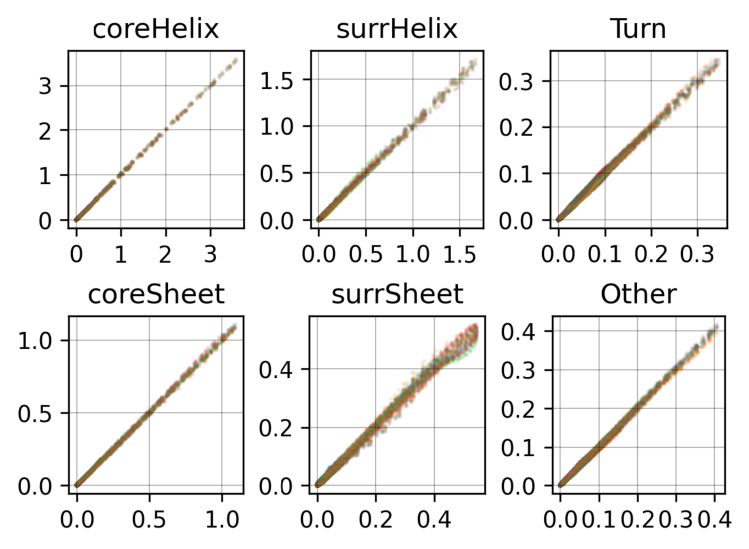
\includegraphics[width=\linewidth]{constava/sup_figs/supfig1.pdf}
    \caption{\textbf{Cross-validation of probability density kernels of conformational states.} The kernels were fitted five times, leaving out 20\% of the ensembles each time. The plots show the correlation between probability densities sampled from the five different kernels.}
    \label{fig:sup_fig_constava:cross_validation}
\end{figure}

\begin{figure}[H]
    \centering
    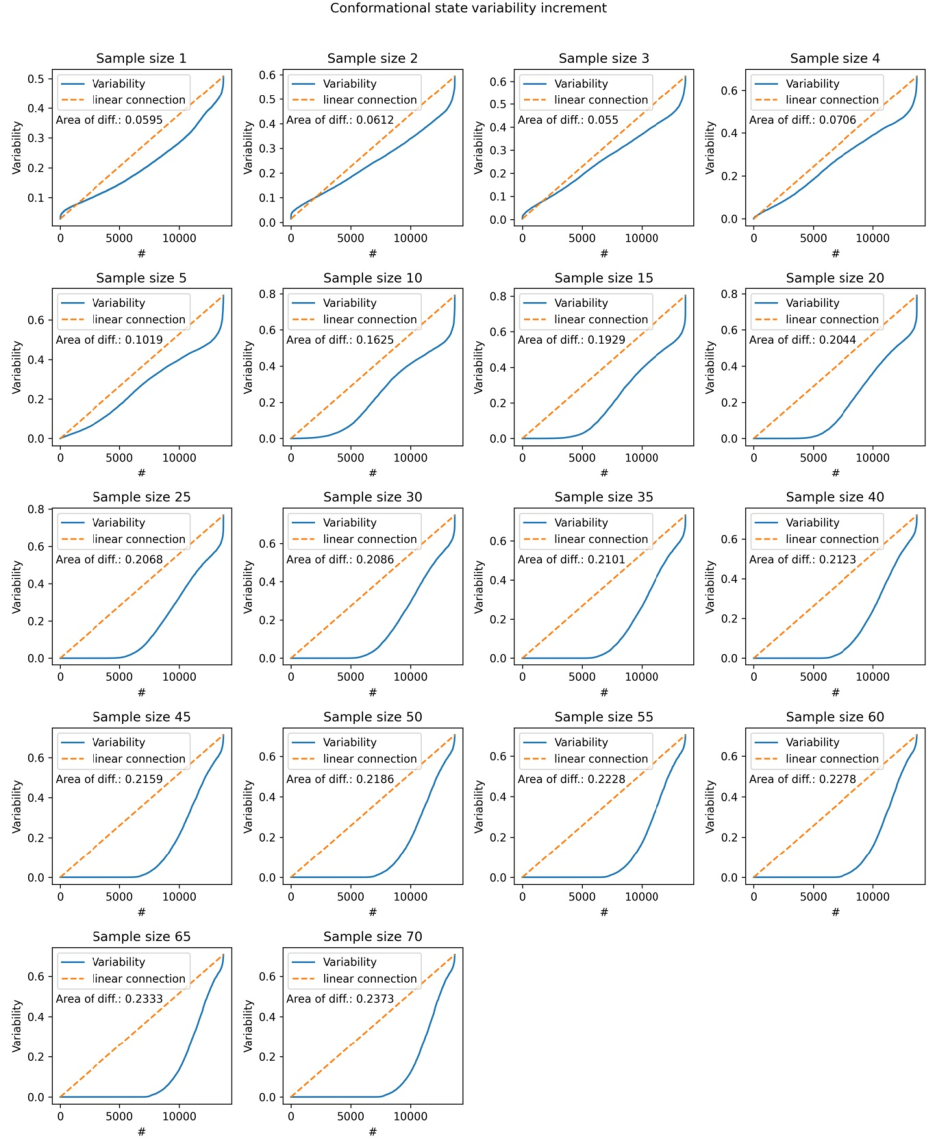
\includegraphics[width=0.9\linewidth]{constava//sup_figs/supfig2.pdf}
    \caption{\textbf{Influence of the sample size on the conformational state variability.} Conformational state variabilities were calculated for all residues in the MD ensembles employing bootstrapping with different sample sizes (10,000 samples). The resulting values were plotted in ascending order (blue), while the dashed line (orange) represents an ideal line between the minimum and maximum values. Thus, the area between the two lines is a measure of the linearity of the conformational state variability in the dataset. As the sample size increases, less samples fall in the linear section of the conformational state variability metric. A sample size of 3 was chosen to obtain informative conformational state variabilities from ensembles for presenting the highest linearity in the metric while also spanning over a decent value range (min-max, see \suppfigref{fig:sup_fig_constava:range}).}
    \label{fig:sup_fig_constava:sample_size}
\end{figure}

\begin{figure}[H]
    \centering
    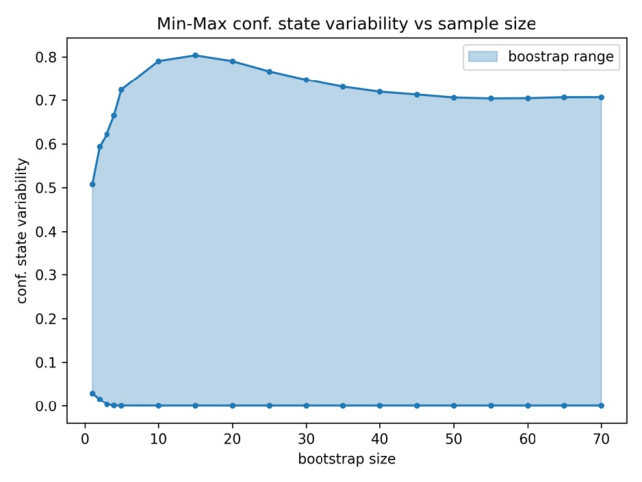
\includegraphics[width=0.9\linewidth]{constava//sup_figs/supfig3.pdf}
    \caption{\textbf{Range of conformational state variability values as a function of the sample size.} Conformational state variabilities were calculated for all residues in the MD ensembles employing bootstrapping with different sample sizes (10,000 samples). The minimum and maximum values are shown here. Initially, as the sample size increases, the range between minimum and maximum values increases as well, reaching a maximum at a sample size of 15. For low sample sizes, conformational state variabilities of 0 are practically not observed. This indicates that even smallest fluctuations of the backbone dihedrals lead to an increase in conformational state variability. As the sample size increase, those small fluctuations become less important, allowing for conformational state variabilities that are practically 0.}
    \label{fig:sup_fig_constava:range}
\end{figure}

\begin{figure}[H]
    \centering
    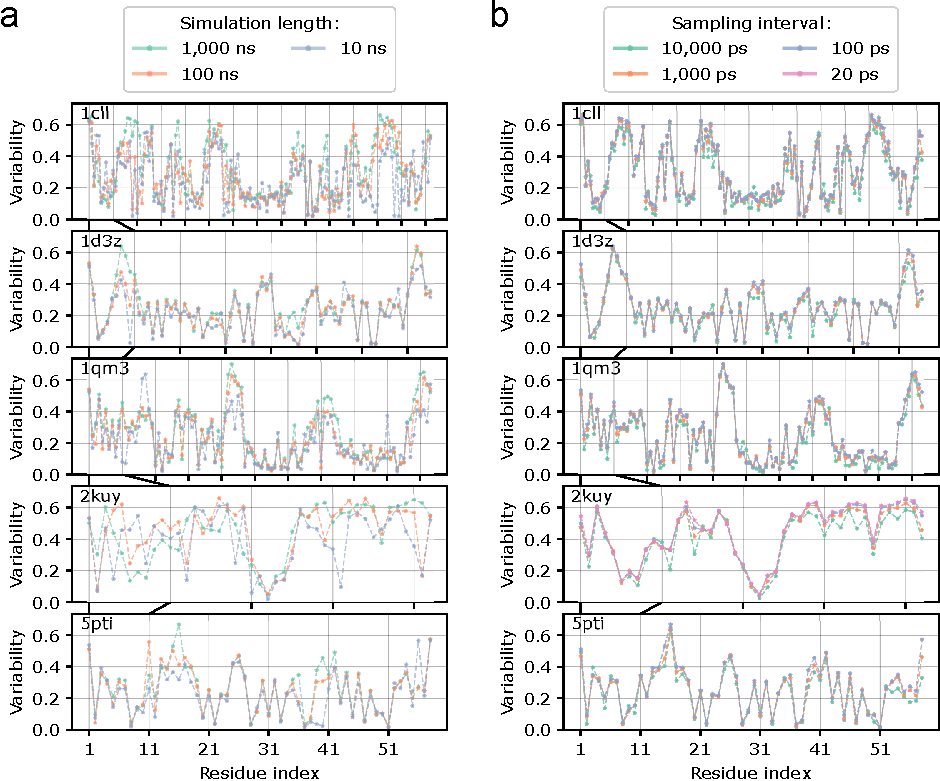
\includegraphics[width=1\linewidth]{constava//sup_figs/supfig4.pdf}
    \caption{\textbf{Analysis of sampling parameters for molecular dynamics simulations.} Five proteins were simulated to assess the impact of different sampling parameters on the results. From all simulations the conformational state variabilities were calculated using the sliding window-approach with a window size of 3. Results are shown as the conformational state variability along the sequence for different sampling parameters. a) Analysis of the of the impact of simulation time. Results after 100 ns did not differ much from longer simulations. b) Analysis of the impact of sampling intervals. Only minor changes were observed. Sampling in intervals of 1,000 ps was chosen for the final simulations in this work, to minimize the autocorrelation between subsequent sampling time points.}
    \label{fig:sup_fig_constava:MD_parameters}
\end{figure}

\begin{figure}[H]
    \centering
    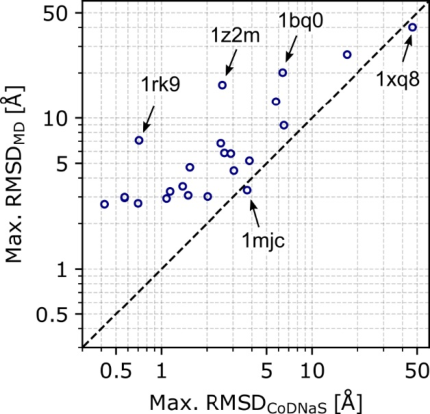
\includegraphics[width=0.7\linewidth]{constava//sup_figs/supfig5.pdf}
    \caption{\textbf{Comparison of conformational diversity between MD ensembles and CoDNaS.} For a given protein the maximum RMSD values between any structures in CoDNaS (x-axis) and the MD ensemble (y-axis) are depicted. With two exceptions (1mjc and 1xq8) the MD simulations produced more diverse ensembles than the structures in CoDNaS. For some structures (e.g., 1z2m and 1bq0) the conformational variability in the simulation strongly exceeded that in CoDNaS. This is mostly due to flexible termini, which MD simulations sample freely. A notable exception is 1rk9, which remains fully folded throughout the simulation but undergoes a conformational change which results in a higher RMSD than observed in CoDNaS. Out of the 113 simulated proteins, only 22 are annotated in CoDNaS.}
    \label{fig:sup_fig_constava:codnas}
\end{figure}

\begin{figure}[H]
    \centering
    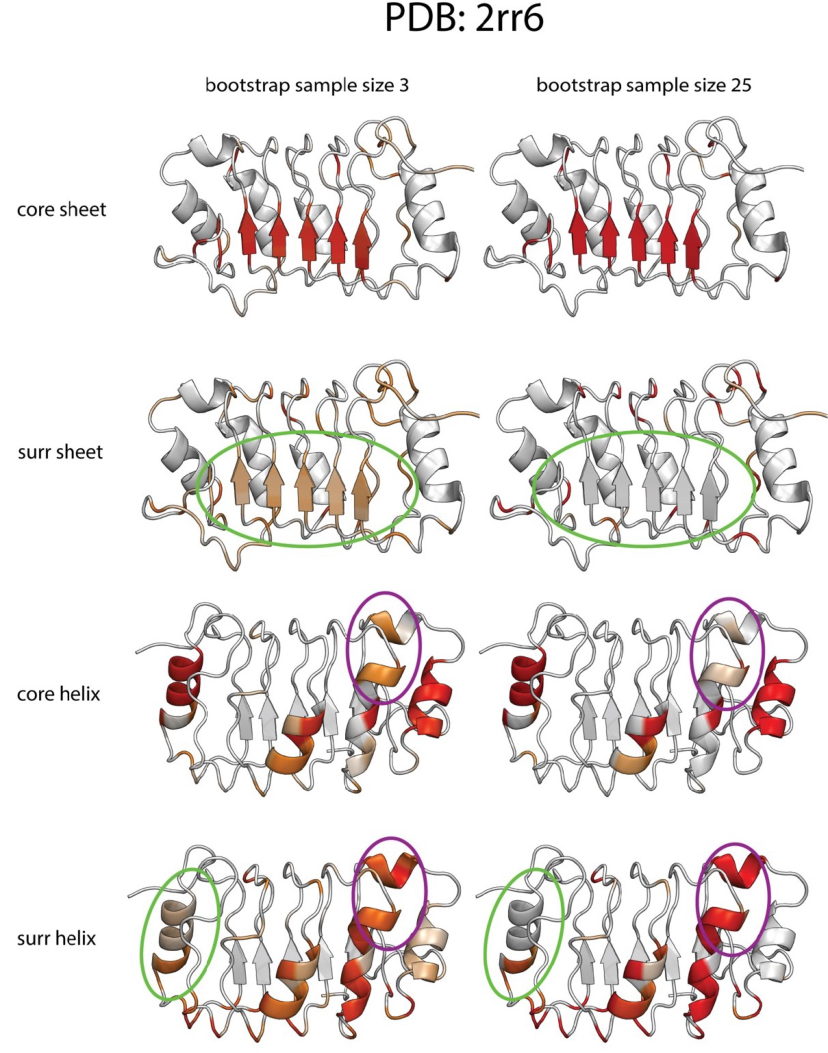
\includegraphics[width=0.8\linewidth]{constava//sup_figs/supfig6.pdf}
    \caption{\textbf{Impact of the sample size on conformational states probabilities in human acidic leucine-rich nuclear phosphoprotein 32 family member B (PDB ID: 2rr6).} Conformational state propensities were inferred from the MD ensembles employing bootstrapping with sample sizes 3 and 25 (10,000 samples). As the sample size increases, ambiguous assignments (shades of orange) become less apparent, rather a preferred conformational state is assigned with high propensity (shades of red). On the first two rows, the low probability for Surrounding sheet in the circled area disappears in favour of higher probabilities towards Core sheet. Similarly, in the last two rows the green circled region experiences an increase in Core helix probability. Contrarily, the purple circled region experiences an increase Surrounding helix probability in detriment of Core helix probability.}
    \label{fig:sup_fig_constava:bootstrap_size}
\end{figure}

\begin{figure}[H]
    \centering
    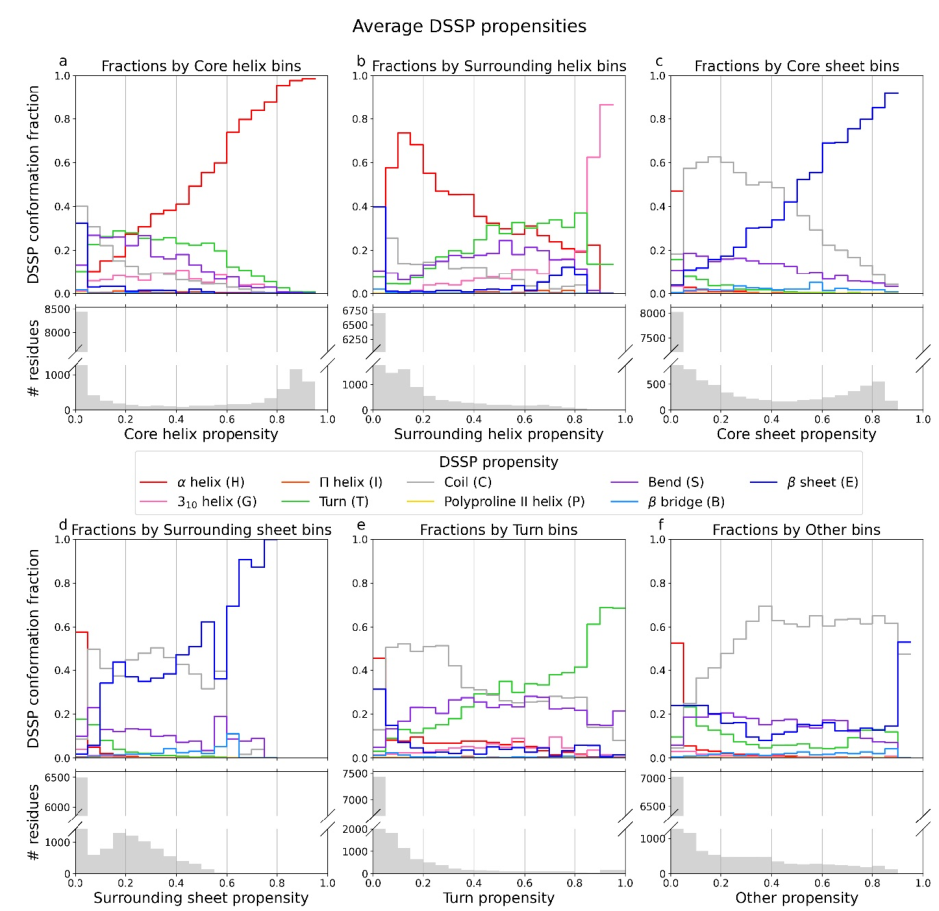
\includegraphics[width=0.9\linewidth]{constava//sup_figs/supfig7.pdf}
    \caption{\textbf{Relation between Constava conformational states and DSSP secondary structure assignments.} Constava conformational state propensities were correlated with DSSP propensities (average fraction of frames assigned to a given secondary structure by DSSP). The two classification schemes were compared in bins. The bar plot below the correlation plots shows the number of samples (residues) in each bin. a) For Core helix propensities there is a correlation to H ($\alpha$-helix). b) For Surrounding helix propensities no clear correlations to any DSSP category can be observed. The values for bins with propensities > 0.8 cannot be properly interpreted due to the low number of samples. c) For Core sheet there is a correlation with E ($\beta$-sheet). d) For Surrounding sheet no clear correlations are apparent. There is some correlation with E, but the relationship is non-linear and the low number of samples for propensities > 0.6 makes the interpretation difficult. e) For Turn a correlation with T (hydrogen bonded turns) emerges but other DSSP categories are observed for all levels of Turn propensity. f) Finally, the Other propensity mostly associates to C (coil), but also other DSSP categories are observed for all levels of Other propensity. Since Turn and Other indicate highly dynamic residues, it makes sense, that these residues form other secondary structure elements transiently.}
    \label{fig:sup_fig_constava:dssp_assignments}
\end{figure}

\begin{figure}[H]
    \centering
    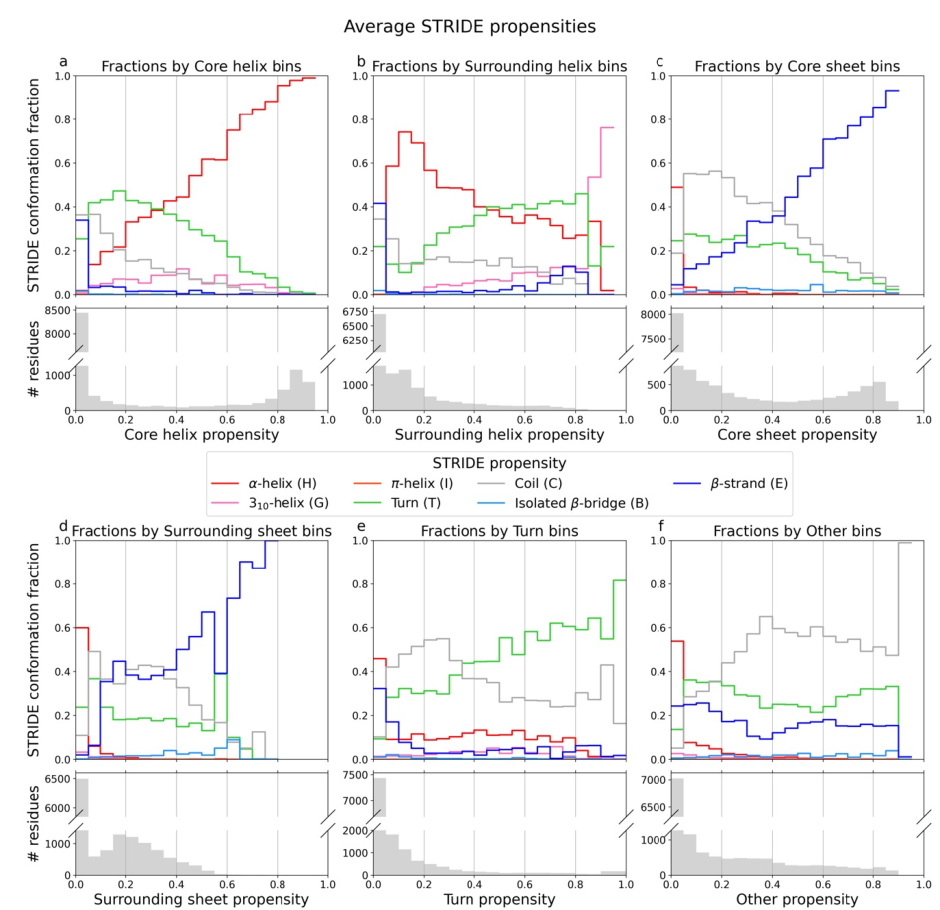
\includegraphics[width=0.9\linewidth]{constava//sup_figs/supfig8.pdf}
    \caption{\textbf{Relation between Constava conformational states and STRIDE secondary structure assignments.} Constava conformational state propensities were correlated with STRIDE propensities (average fraction of frames assigned to a given secondary structure by STRIDE). The two classification schemes were compared in bins. The bar plot below the correlation plots shows the number of samples (residues) in each bin. a) For Core helix propensities there is a correlation to H ($\alpha$-helix). b) For Surrounding helix propensities no clear correlations to any STRIDE category can be observed. The values for bins with propensities > 0.8 cannot be properly interpreted due to the low number of samples. c) For Core sheet there is a correlation with E ($\beta$-sheet). d) For Surrounding sheet no clear correlations are apparent. There is some correlation with E, but the relationship is non-linear and the low number of samples for propensities > 0.6 makes the interpretation difficult. e) For Turn a correlation with T (hydrogen bonded turns) emerges but other STRIDE categories are observed for all levels of Turn propensity. f) Finally, the Other propensity mostly associates to C (coil), but also other STRIDE categories are observed for all levels of Other propensity. Since Turn and Other indicate highly dynamic residues, it makes sense, that these residues form other secondary structure elements transiently.}
    \label{fig:sup_fig_constava:stride_assignments}
\end{figure}

\begin{figure}[H]
    \centering
    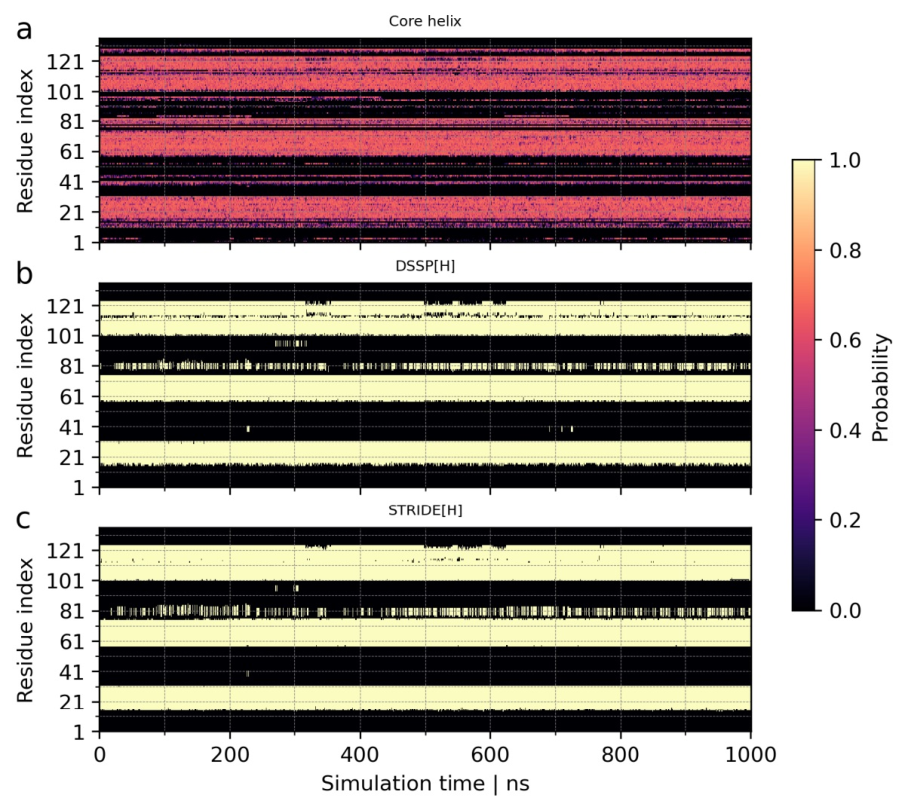
\includegraphics[width=\linewidth]{constava//sup_figs/supfig9.pdf}
    \caption{\textbf{Comparison of Constava and traditional secondary structure assignments with respect to their ability to detect transiently forming secondary structure elements. }
    % Constava, DSSP, and STRIDE were applied to all conformations in the MD trajectories. Shown are: a) Core helix propensities, b) DSSP H ($\alpha$-helix) assignments, and c) STRIDE H ($\alpha$-helix) assignments along the MD trajectory of Endonuclease V (PDB ID: 2end). Beyond the relation between propensities and fractions in Supplementary Fig. 7 and Supplementary Fig. 8, Constava shows the capability to detect conformational states before the criteria for the other methods are met. In addition to returning high Core helix probability to the stable helix regions that DSSP and STRIDE assign, some regions with more dynamic behaviour interestingly show detection of helix propensity. The region between amino acids 95-101 is detected to have notable Core helix propensity (a) by Constava throughout the totality of the simulation, even though it is rarely assigned by DSSP (b) and STRIDE (c) in the MD time steps. Additionally, the region between amino acids 39-45 shows a similar tendency, with a longer amino acid range of high Core helix propensities near in the 300 ns time step, where DSSP and STRIDE detect $\alpha$-helix. This longer stretch indicates that enough amino acids to form the necessary hydrogen bonds for DSSP and STRIDE assignment have adopted Core helix conformation. Finally, the region between amino acids 55-60 is also detected along the whole simulation, while DSSP and STRIDE intermittently assigns $\alpha$-helix.
    }
    \label{fig:sup_fig_constava:detect_trasient}
\end{figure}

\begin{figure}[H]
  \ContinuedFloat
  \caption[]{(Continuation) Constava, DSSP, and STRIDE were applied to all conformations in the MD trajectories. Shown are: a) Core helix propensities, b) DSSP H ($\alpha$-helix) assignments, and c) STRIDE H ($\alpha$-helix) assignments along the MD trajectory of Endonuclease V (PDB ID: 2end). Beyond the relation between propensities and fractions in Supplementary Fig. 7 and Supplementary Fig. 8, Constava shows the capability to detect conformational states before the criteria for the other methods are met. In addition to returning high Core helix probability to the stable helix regions that DSSP and STRIDE assign, some regions with more dynamic behaviour interestingly show detection of helix propensity. The region between amino acids 95-101 is detected to have notable Core helix propensity (a) by Constava throughout the totality of the simulation, even though it is rarely assigned by DSSP (b) and STRIDE (c) in the MD time steps. Additionally, the region between amino acids 39-45 shows a similar tendency, with a longer amino acid range of high Core helix propensities near in the 300 ns time step, where DSSP and STRIDE detect $\alpha$-helix. This longer stretch indicates that enough amino acids to form the necessary hydrogen bonds for DSSP and STRIDE assignment have adopted Core helix conformation. Finally, the region between amino acids 55-60 is also detected along the whole simulation, while DSSP and STRIDE intermittently assigns $\alpha$-helix.}
\end{figure}

\begin{figure}[H]
    \centering
    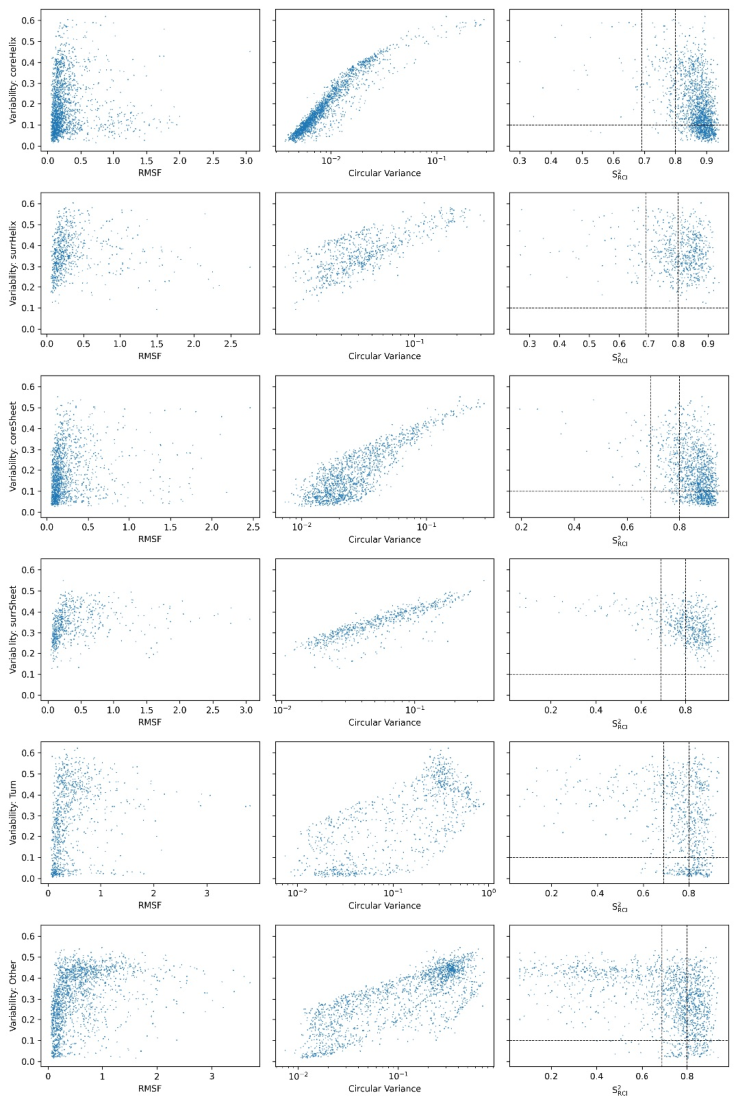
\includegraphics[width=0.85\linewidth]{constava//sup_figs/supfig10.pdf}
    \caption{\textbf{Comparison of conformational state variability with traditional dynamics metrics per prevalent conformational state.} 
    % Conformational state propensities were inferred from the MD ensembles employing bootstrapping with sample sizes 3 (10,000 samples). The results were subdivided by their prevalent conformational state. From top to bottom these are: Core helix, Surrounding helix, Core sheet, Surrounding sheet, Turn and Other. In the left column, the conformational state variability is potted against the root mean square fluctuations (RMSF). In the central column, the conformational state variability is plotted against the circular variance. On the right, the conformational state variability is plotted against the $\text{S}^{2}_{RCI}$. The vertical dotted lines indicate the border between likely disordered, context-dependent and ordered residues (left to right) as defined in previous work [1]. The horizontal dotted line is a visual guide to distinguish between residues with very low and higher conformational state variability.
    }
    \label{fig:sup_fig_constava:metrics}
\end{figure}

\begin{figure}[H]
  \ContinuedFloat
  \caption[]{(Continuation) Conformational state propensities were inferred from the MD ensembles employing bootstrapping with sample sizes 3 (10,000 samples). The results were subdivided by their prevalent conformational state. From top to bottom these are: Core helix, Surrounding helix, Core sheet, Surrounding sheet, Turn and Other. In the left column, the conformational state variability is potted against the root mean square fluctuations (RMSF). In the central column, the conformational state variability is plotted against the circular variance. On the right, the conformational state variability is plotted against the $\text{S}^{2}_{RCI}$. The vertical dotted lines indicate the border between likely disordered, context-dependent and ordered residues (left to right) as defined in previous work [1]. The horizontal dotted line is a visual guide to distinguish between residues with very low and higher conformational state variability.}
\end{figure}

\begin{figure}[H]
    \centering
    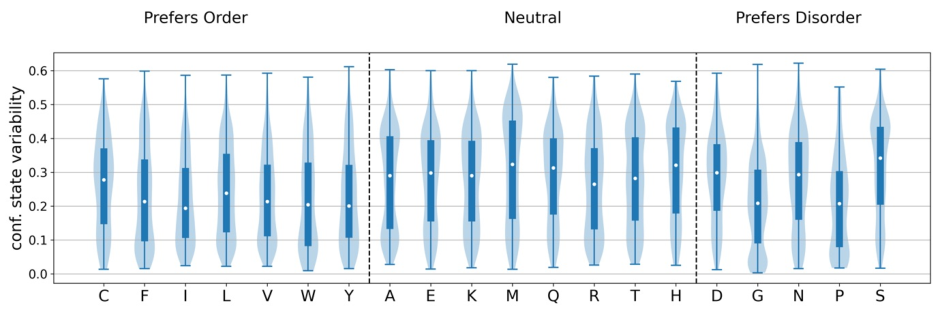
\includegraphics[width=1\linewidth]{constava//sup_figs/supfig11.pdf}
    \caption{\textbf{Conformational state variability values per amino acid type according to their order preference, terminal regions included.} Conformational state variabilities were calculated for all residues in the MD ensembles employing bootstrapping with sample size 3 (10,000 samples). Amino acids were classified depending on their intrinsic order preference according to the classification on previous work1 as preferentially ordered (cysteine, phenylalanine, isoleucine, leucine, valine, tryptophan \& tyrosine), neutral (alanine, glutamic acid, lysine, methionine, glutamine, arginine, threonine \& histidine) and preferentially disordered (aspartic acid, glycine, asparagine, proline \& serine). Amino acids which prefer order generally featured lower conformational state variability values than the remaining. The homologous figure with terminal residues removed can be found in the main text, Figure 5. This figure mainly differs in the variability values distribution for methionine, which features higher values in this figure than in Figure 6. This is due to the preferential location of Methionine at the N-terminal region of the protein, which is less bound to inter-residue interactions and allows for easier conformational state changes and therefore variability.}
    \label{fig:sup_fig_constava:aa_order}
\end{figure}

\begin{figure}[H]
    \centering
    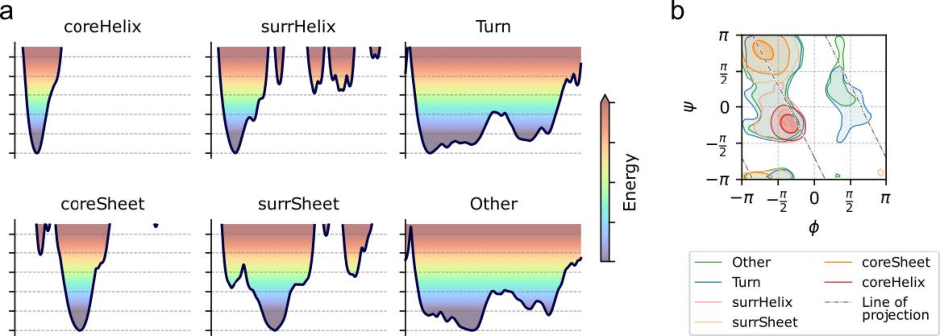
\includegraphics[width=1\linewidth]{constava//sup_figs/supfig12.pdf}
    \caption{\textbf{Schematic representation of the conformational states as energy landscapes.} a) Cross section through the energy landscapes along the line of projection (shown in panel b). coreHelix and coreSheet conformational states are defined by a single deep energy well, vastly restricting backbone mobility. The states surrHelix and surrSheet show lowered energy barriers, allowing for more backbone mobility. Finally, in the Other and Turn conformational states, most of the dihedral space is accessible with only minor energy barriers in between. b) Schematic overview of the definition of the conformational states, as well as the line of projection used in panel a.}
    \label{fig:sup_fig_constava:2d_landscape}
\end{figure}

\begin{figure}[H]
    \centering
    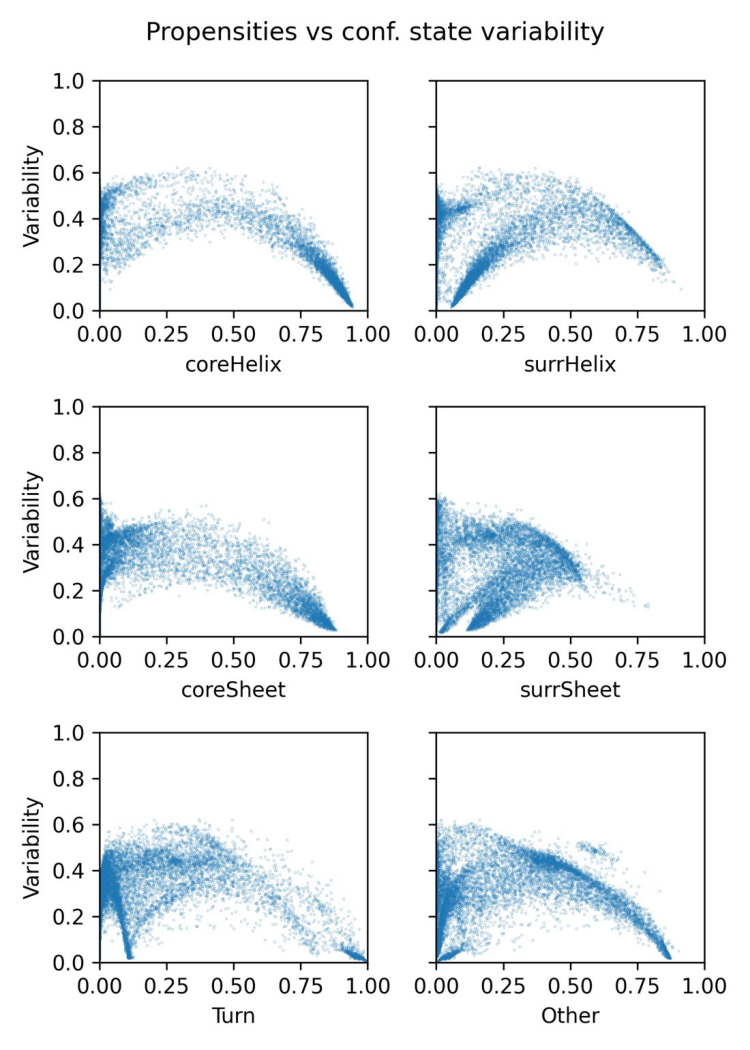
\includegraphics[width=0.8\linewidth]{constava//sup_figs/supfig13.pdf}
    \caption{\textbf{Conformational states propensities vs conformational state variability.} The metrics were calculated using bootstrapping with a sample size of 3 (10,000 samples). Conformational state propensities for each conformational state are plotted on the x axes, while the y axes show the conformational state variability. As the conformational state propensity for a single conformational state approaches 1, the conformational state variability drops to 0. In contrast, no such correlation can be observed in the left half of the plots. As the probability for a given conformational state approaches 0, the residue may still assume any of the remaining five states, and transition between them, thus, allowing for no conclusions on the conformational state variability.}
    \label{fig:sup_fig_constava:var_vs_propensity}
\end{figure}

\begin{figure}[H]
    \centering
    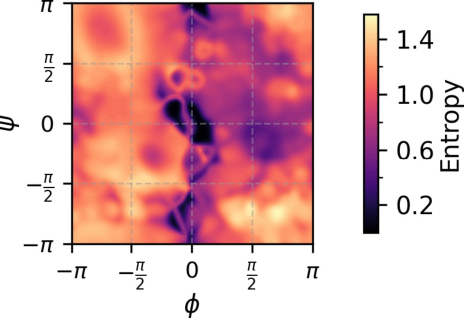
\includegraphics[width=0.8\linewidth]{constava//sup_figs/supfig14.pdf}
    \caption{\textbf{Entropy of the conformational states in the ($\phi$, $\psi$)-space.} The entropy is a measure of how sensitive the conformational states are to minor changes in the backbone dihedrals in the corresponding areas. The area around (0, 0) is not populated in any of the conformational state models. Thus, the entropy in this region approaches 0.}
    \label{fig:sup_fig_constava:entropy}
\end{figure}

\begin{figure}[H]
    \centering
    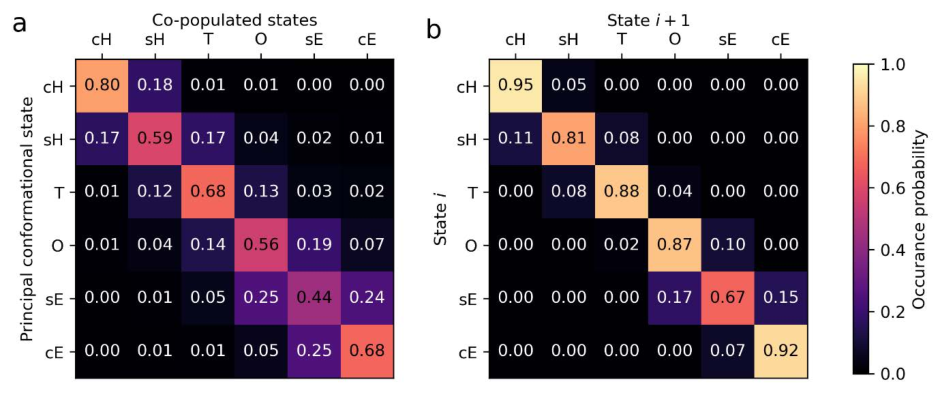
\includegraphics[width=1\linewidth]{constava//sup_figs/supfig15.pdf}
    \caption{\textbf{Co-occurrence of conformational states.} a) This plot shows the overall co-occurrence of conformational states in individual residues. For every residue with a given most likely conformational state (vertical axis), the average remaining propensities for all other states are shown (horizontal axis). b) This plot shows the probabilities of residues transitioning between conformational states between two subsequent time points. Both plots were obtained with window size 3. The labels correspond to the conformational states as follows: cH (Core helix), sH (Surrounding helix), T (Turn), O (Other), sE (Surrounding sheet), cE (Core sheet).}
    \label{fig:sup_fig_constava:co-occurrence}
\end{figure}

\newpage

\begin{suppdata} \label{data:sup_data_constava:order_class_proteins}
\textbf{List of proteins according to order class.}\\

\noindent\textbf{Disordered:} 2aqc, 1xq8, 1mjc, 1u96, 1ss3, 2kbz, 2l95, 1nq4, 1vd0, 1y00, 1rk9, 2l50, 1yob, 1rqs, 1czh.\\
\textbf{Half-disordered:} 2jo6, 2rvh, 2khz, 1akp, 2m2u, 2ho9, 2m9v, 2joy, 2mlw, 2lnu, 1b75, 2ot2, 1c9h, 2l7w, 1r1t, 2l49, 2l9n, 2myi, 2ls7, 1o13, 2lvh, 2l6o, 5vo7, 2kly, 2l25, 1wm2, 2kpq, 2kg7, 1l7y, 2gqb, 1eni, 1z2m, 2den, 2jra, 2jyz, 2jz4, 2m0y, 2m2a, 2mc9, 2mhe, 2mvz, 2x8n, 4beh, 4eyv, 5jtk.\\
\textbf{Structured:} 2mkx, 1jqr, 2fm4, 1jw3, 2rr6, 1hg7, 1sp0, 2kva, 3hnx, 1tm9, 1om2, 2d49, 2hfi, 1ufn, 1qkh, 2fvt, 1rzs, 1x3a, 1ey1, 1wjt, 2hgk, 2k2t, 2jny, 2jso, 2rn4, 1bq0, 1g9l, 1imq, 1iyr, 1jh3, 1jw2, 1mp1, 1nnv, 1nzp, 1rq6, 1rrz, 1ryk, 1t0g, 1tl6, 1v66, 1v9v, 1xhs, 2ebm, 2end, 2gbs, 2hfq, 2jgx, 2jov, 2jrr, 2jv2, 2jzv, 2ken, 2lfj.
\end{suppdata}

\begin{suppdata} \label{data:sup_data_constava:prots_with_nmr_metrics}
\textbf{List of proteins mapped to NMR metrics.} Only the following subset of MD proteins had their corresponding Random Coil Index information available:\\

\noindent2m2a, 1jw2, 2ls7, 1t0g, 2jny, 1tm9, 1v66, 2gqb, 2ebm, 2kpq, 1ryk, 2gbs, 2fvt, 2ken, 1b75, 2l25, 2rr6, 1iyr, 2hfi, 2ho9, 1akp, 2fm4, 1xhs, 1l7y, 1ufn, 2mlw, 1ey1, 2kva, 2mvz, 2lnu, 2lfj, 1om2, 2jyz, 2mhe, 1v9v, 2l49, 1jqr, 1x3a, 1g9l, 2rvh, 5vo7, 1bq0, 2l6o, 1c9h, 2jov, 2ot2, 2joy, 2rn4, 2hgk, 1jh3, 2jz4, 5jtk, 1rzs, 2jso, 2kbz, 1rq6, 2jzv, 1wjt, 1jw3, 2jrr, 1hg7, 1imq.
\end{suppdata}

% \chapter*{Supplementary information chapter \ref{chapter:plddt}: \\NMR-derived}
\chapter*{Supplementary information chapter 5: \\NMR-derived}
\setcounter{chapter}{5}
\addcontentsline{toc}{chapter}{Supplementary information chapter 5}
% \addcontentsline{toc}{chapter}{Supplementary information chapter \ref{chapter:plddt}}
\markright{SUPPLEMENTARY INFORMATION}

\setcounter{figure}{0} % Reset the figure counter
\renewcommand{\figurename}{Supplementary Fig.}

\setcounter{table}{0} % Reset the figure counter
\renewcommand{\tablename}{Supplementary Table}

\newpage


\begin{figure}[H]
    \centering
    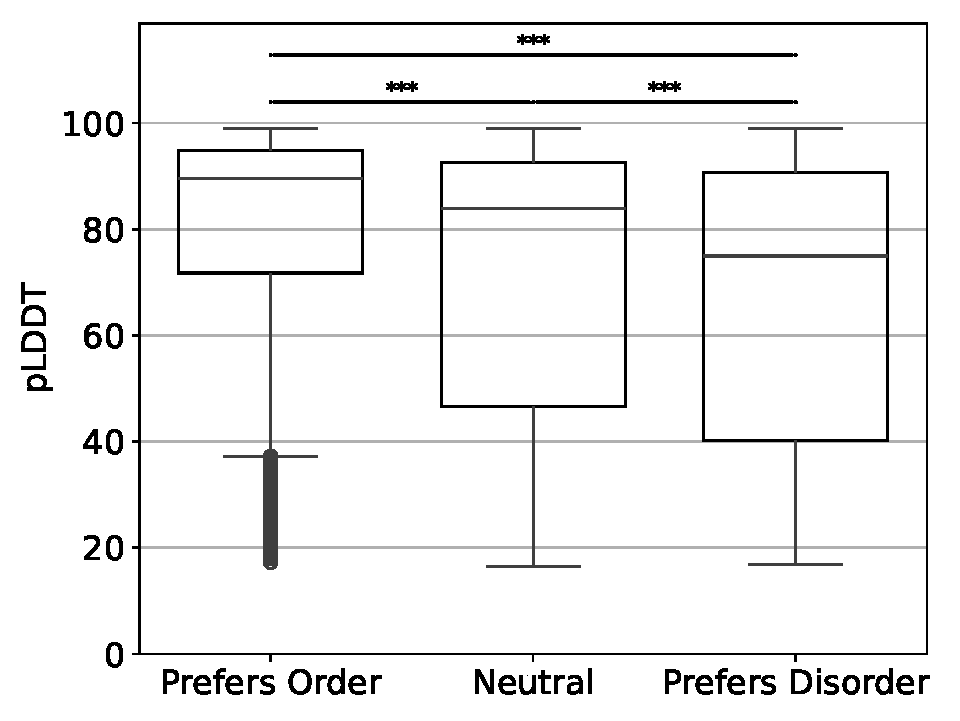
\includegraphics[width=0.8\textwidth]{pLDDT/plddt_figures/box_plot_rciset_plddt_dynamine_classes.pdf}
    \caption{\textbf{pLDDT values per amino acid order classes.} The amino acids from the $S^{2}_{\text{RCI}}$ dataset were clustered in 3 classes according to their order preference: preferentially ordered (cysteine, phenylalanine, isoleucine, leucine, valine, tryptophan \& tyrosine; N=106,363), neutral (alanine, glutamic acid, lysine, methionine, glutamine, arginine, threonine \& histidine; N=155,050) and preferentially disordered (aspartic acid, glycine, asparagine, proline \& serine; N=112,945). The distributions were tested with a Mann–Whitney U test, which resulted in p-values < 0.001 in all tests.}
    \label{fig:plddt_aa_classes_boxplot}
\end{figure}


\begin{figure}[H]
    \centering
    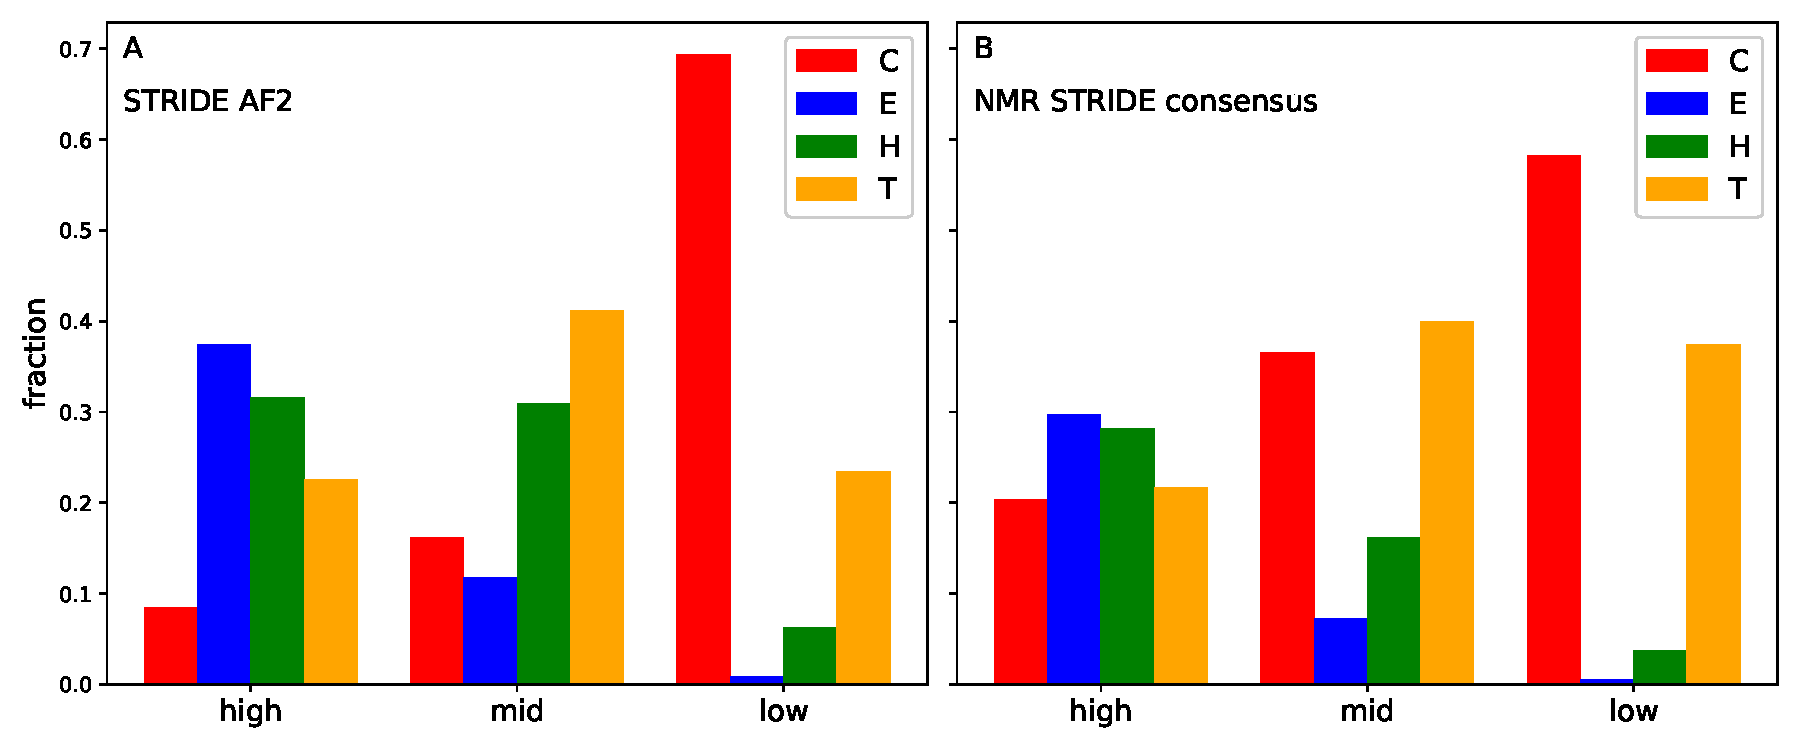
\includegraphics[width=\textwidth]{pLDDT/plddt_figures/barplot_plddt_regions_per_ss_type_abundance_only_normalised_af_stride_af_ss_nmr_strideCons.pdf}
    \caption{\textbf{Abundance of secondary structures by pLDDT ranges.} A) The STRIDE secondary structure assignment from the structure that AlphaFold2 produces. B) The STRIDE consensus secondary structure assignment here provided is the most abundantly assigned secondary structure in the ensemble of NMR structures available. The STRIDE consensus assignment (panel B) produces a decrease in abundance for helix (H) and sheet (E) fractions as the pLDDT decreases, as well as an increase in coil (C) and turn (T) conformations. These tendencies are maintained for AlphaFold2's single structure assignment (panel A) in sheet and coil fractions, but not for helix and turn.}
    \label{fig:ss_barplots_normalised}
\end{figure}




\begin{figure}[H]
    \centering
    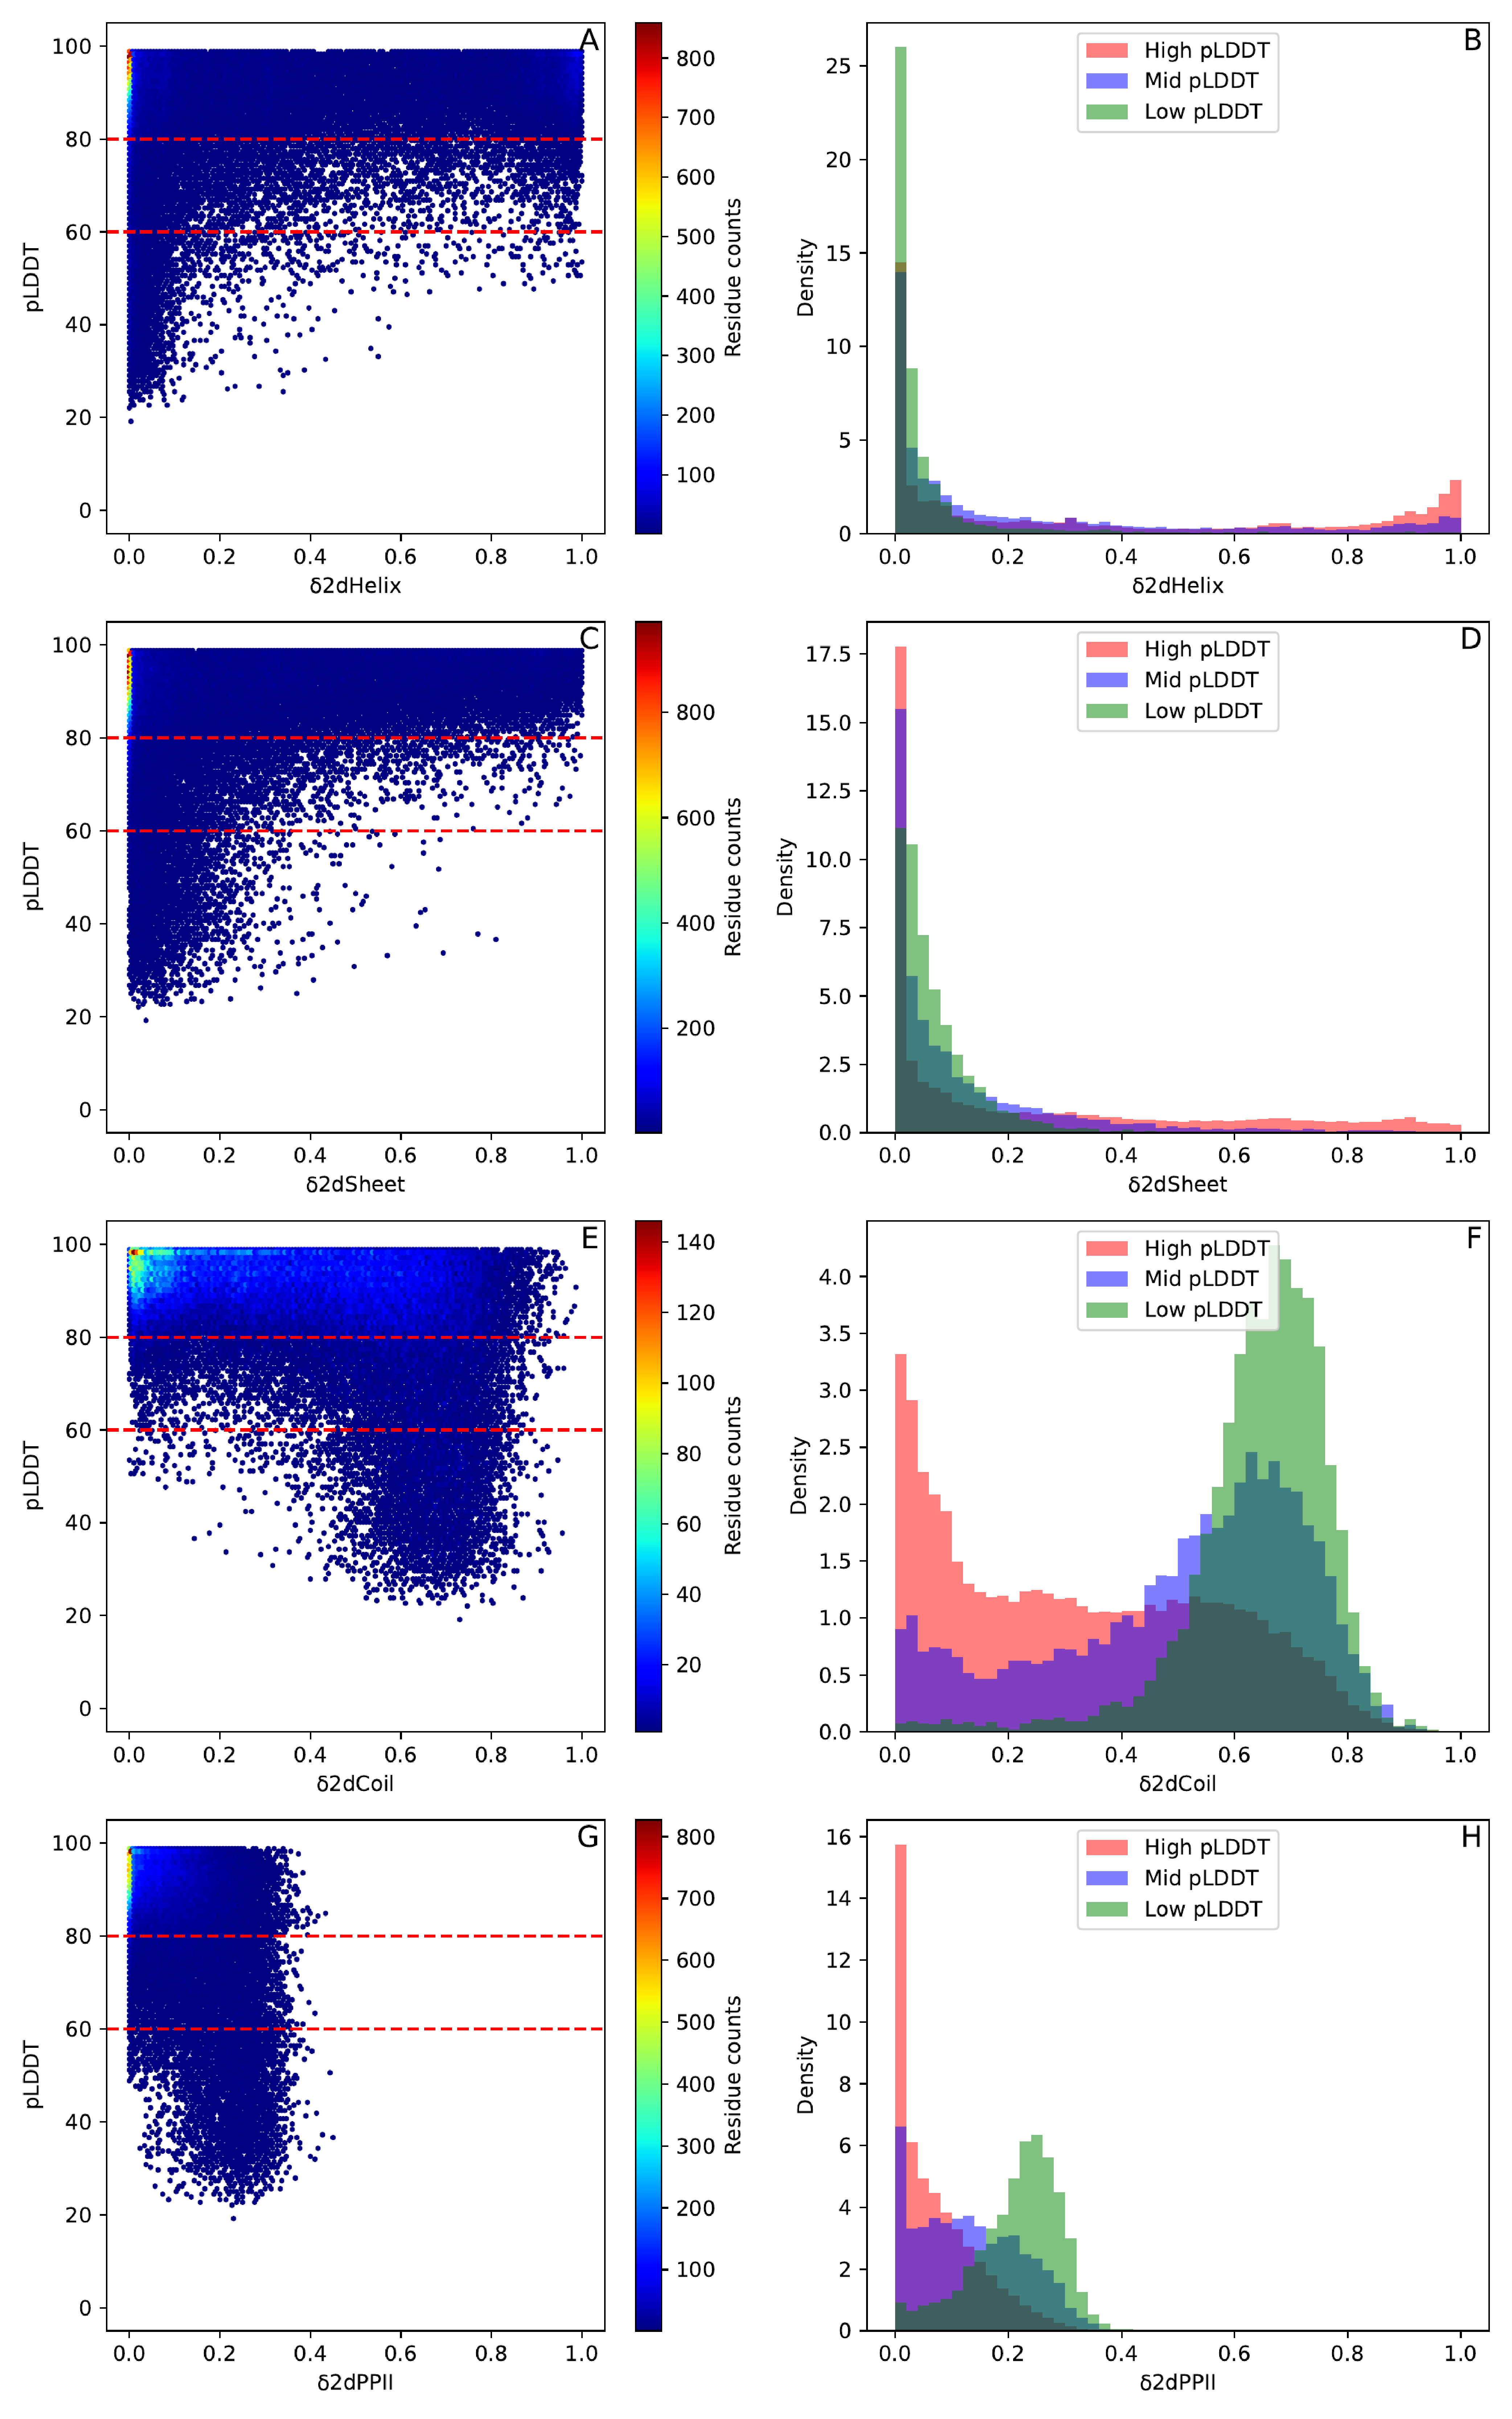
\includegraphics[width=0.85\textwidth]{pLDDT/plddt_figures/plddt_vs_d2d_hexbin_hist_undivided.pdf}
    \caption{\textbf{Comparison of pLDDT and $\delta 2D$ populations.} Caption in next page. 
    % For all available residues in the $S^{2}_{\text{RCI}}$ dataset, the populations of conformational states were calculated with $\delta$2D method. High populations values of a conformation indicate high presence of such conformation in the ensemble, and vice-versa. A-D: For both Helix and Sheet conformations, higher $\delta$2D populations are obtained for residues featuring high pLDDT  (\( \geq 80 \), N=62,014), gradually adopting lower populations for mid (\( 80 > \text{pLDDT} \geq 60 \), N=8,539) and low (\( < 60 \), N=4,773) pLDDT values. E-H: Coil and PPII populations are prominently higher for higher for low pLDDT ranges than for mid and high ranges. 
    % Mann-Whitney two-sided U tests p-values between each pLDDT-stratified distribution for each $\delta 2D$ conformation confirmed difference at p-values < 0.001 (table \ref{table:mann_whitney_results_delta2d}).
    }
    \label{fig:plddt_vs_d2d_undivided}
\end{figure}

\begin{figure}[H]
  \ContinuedFloat
  \caption[]{(Continuation) For all available residues in the $S^{2}_{\text{RCI}}$ dataset, the populations of conformational states were calculated with $\delta$2D method. High populations values of a conformation indicate high presence of such conformation in the ensemble, and vice-versa. A-D: For both Helix and Sheet conformations, higher $\delta$2D populations are obtained for residues featuring high pLDDT  (\( \geq 80 \), N=62,014), gradually adopting lower populations for mid (\( 80 > \text{pLDDT} \geq 60 \), N=8,539) and low (\( < 60 \), N=4,773) pLDDT values. E-H: Coil and PPII populations are prominently higher for higher for low pLDDT ranges than for mid and high ranges. 
    Mann-Whitney two-sided U tests p-values between each pLDDT-stratified distribution for each $\delta 2D$ conformation confirmed difference at p-values < 0.001 (\supptableref{table:mann_whitney_results_delta2d}).}
\end{figure}


\begin{figure}[H]
    \centering
    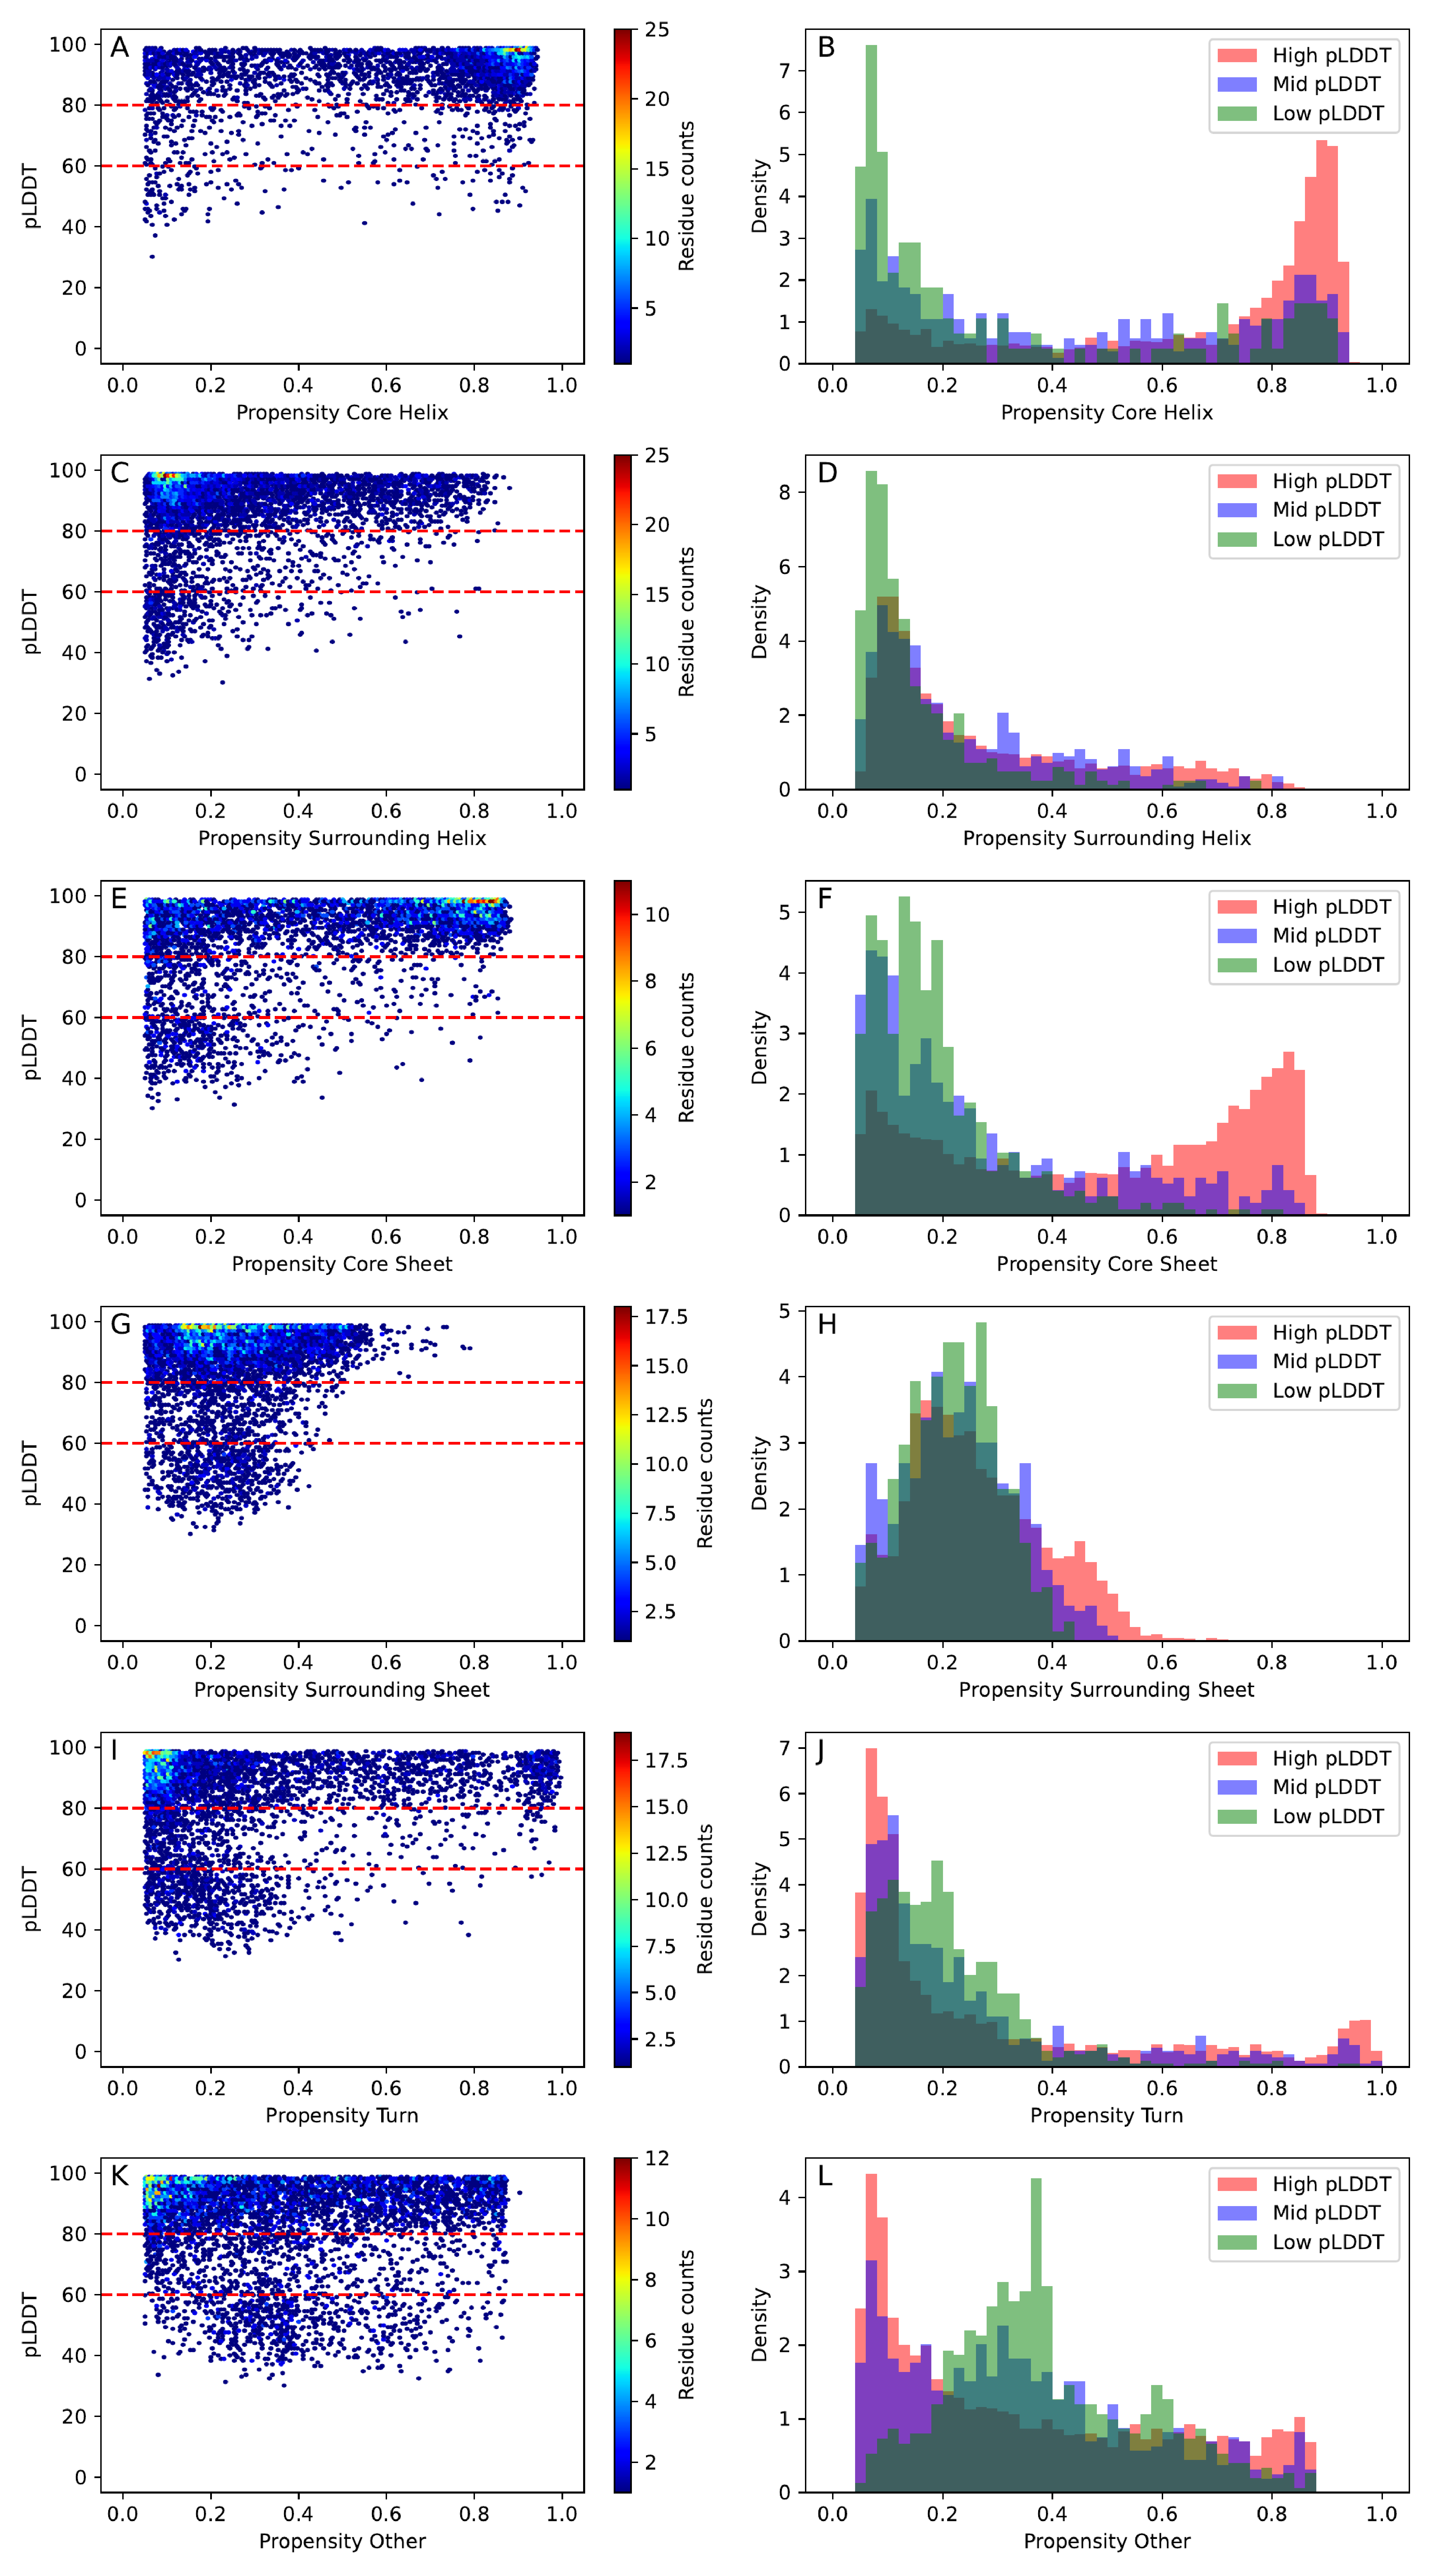
\includegraphics[width=0.8\textwidth]{pLDDT/plddt_figures/plddt_vs_conformational_state_propensities_hexbin_complete_hist.pdf}
    \caption{
    \textbf{Comparison between AlphaFold2 pLDDT and Constava's conformational state propensities.} Caption in next page. 
    % The pLDDT of each residue was plotted against the propensity for each of the 6 conformational states calculated in Constava. Any propensity below 0.05 was deemed non-informative and discarded to facilitate interpretation. 
    % All residues in the MD dataset were stratified in  high (N=9,523), mid (N=1,038) and low (N=809) AlphaFold2 ranges. 
    % A \& B) Hexagonal binning of AlphaFold3 C-$\alpha$ pLDDT vs Core Helix propensity and its associated pLDDT-stratified distributions. 
    % C \& D) Hexagonal binning of AlphaFold3 C-$\alpha$ pLDDT vs Surrounding Helix propensity and its associated pLDDT-stratified distributions. 
    % E \& F) Hexagonal binning of AlphaFold3 C-$\alpha$ pLDDT vs Core Sheet propensity and its associated pLDDT-stratified distributions. 
    % G \& H) Hexagonal binning of AlphaFold3 C-$\alpha$ pLDDT vs Surrounding Sheet propensity and its associated pLDDT-stratified distributions. 
    % I \& J) Hexagonal binning of AlphaFold3 C-$\alpha$ pLDDT vs Turn propensity and its associated pLDDT-stratified distributions. 
    % K \& L) Hexagonal binning of AlphaFold3 C-$\alpha$ pLDDT vs Other propensity and its associated pLDDT-stratified distributions. 
    % The p-values for the Mann-Whitney two-sided U tests between each pLDDT-stratified distribution for every conformational state can be found in supplementary table \ref{table:mann_whitney_results_md}.
    }
\label{fig:plddt_vs_constava_propensities}
\end{figure}

\begin{figure}[H]
  \ContinuedFloat
  \caption[]{ (Continuation) The pLDDT of each residue was plotted against the propensity for each of the 6 conformational states calculated in Constava. Any propensity below 0.05 was deemed non-informative and discarded to facilitate interpretation. 
    All residues in the MD dataset were stratified in  high (N=9,523), mid (N=1,038) and low (N=809) AlphaFold2 ranges. 
    A \& B) Hexagonal binning of AlphaFold3 C-$\alpha$ pLDDT vs Core Helix propensity and its associated pLDDT-stratified distributions. 
    C \& D) Hexagonal binning of AlphaFold3 C-$\alpha$ pLDDT vs Surrounding Helix propensity and its associated pLDDT-stratified distributions. 
    E \& F) Hexagonal binning of AlphaFold3 C-$\alpha$ pLDDT vs Core Sheet propensity and its associated pLDDT-stratified distributions. 
    G \& H) Hexagonal binning of AlphaFold3 C-$\alpha$ pLDDT vs Surrounding Sheet propensity and its associated pLDDT-stratified distributions. 
    I \& J) Hexagonal binning of AlphaFold3 C-$\alpha$ pLDDT vs Turn propensity and its associated pLDDT-stratified distributions. 
    K \& L) Hexagonal binning of AlphaFold3 C-$\alpha$ pLDDT vs Other propensity and its associated pLDDT-stratified distributions. 
    The p-values for the Mann-Whitney two-sided U tests between each pLDDT-stratified distribution for every conformational state can be found in \supptableref{table:mann_whitney_results_md}.}
\end{figure}

\newpage

\begin{figure}[H]
    \centering
    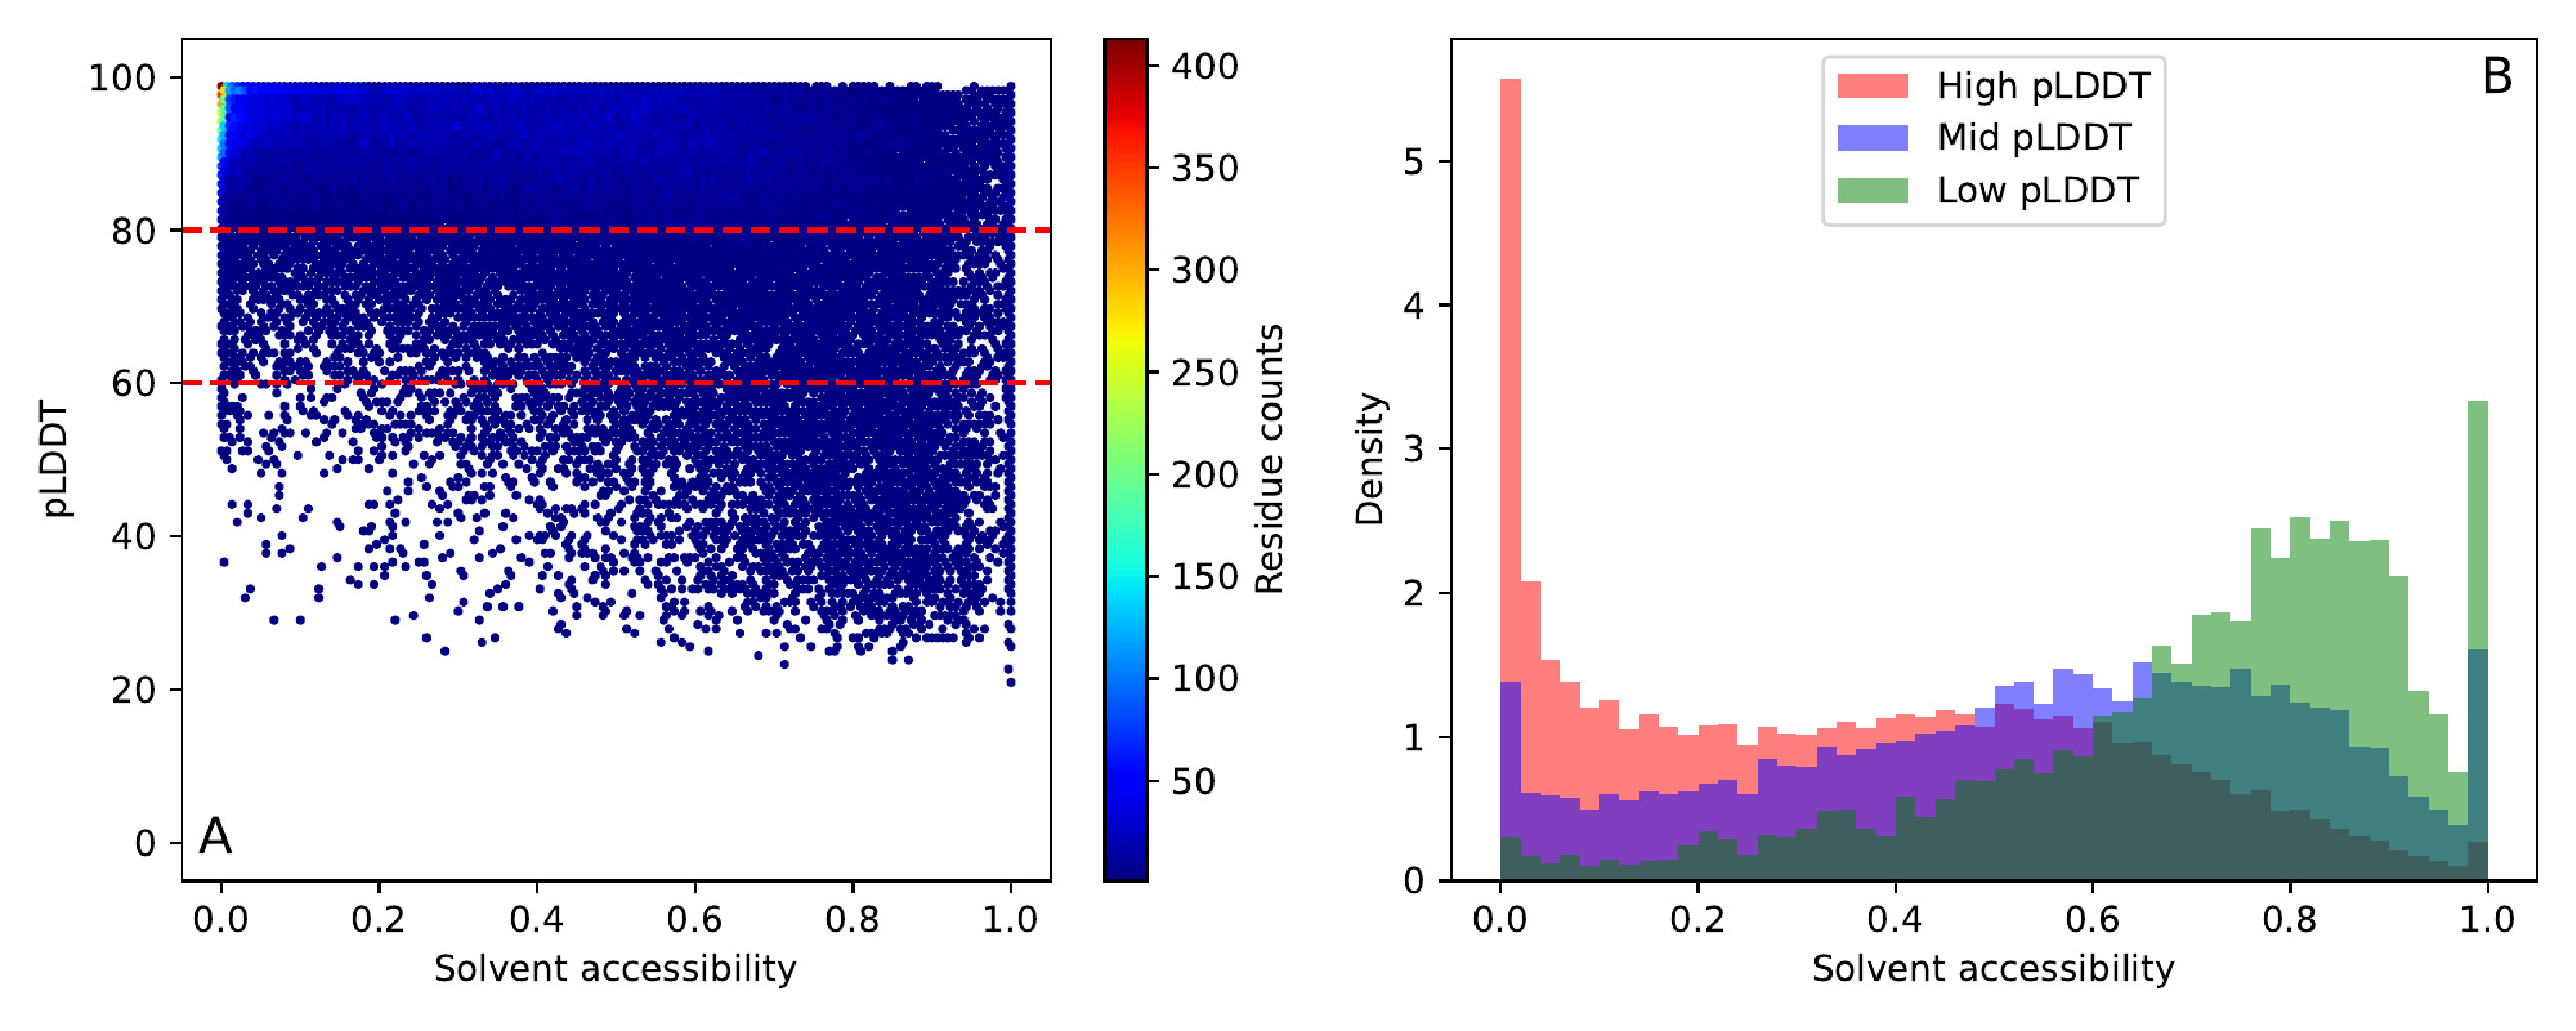
\includegraphics[width=\textwidth]{pLDDT/plddt_figures/plddt_vs_solvent_accessibility_hexbin_hist_undivided.pdf}
    \caption{\textbf{Comparison of pLDDT and solvent accessibility.}
    A) The AlphaFold2 pLDDT in the $S^{2}_{RCI}$ dataset were plotted against the solvent accessibility score for every residue with available values, in an hexagonal binning plot.
    B) Distributions of solvent accessibility scores, stratified in high (\( \geq 80 \), N=62,319), mid (\( 80 > \text{pLDDT} \geq 60 \), N=8,708) and low (\( < 60 \), N=4,842) AlphaFold2 pLDDT values. 
    Mann-Whitney two-sided U test confirmed significant differences between all distribution pairs with a p-value \( < 0.001 \) (\supptableref{table:mann_whitney_results}).
    }
\label{fig:plddt_vs_solvent_accesibility_undivided}
\end{figure}



\begin{figure}[H]
    \centering
    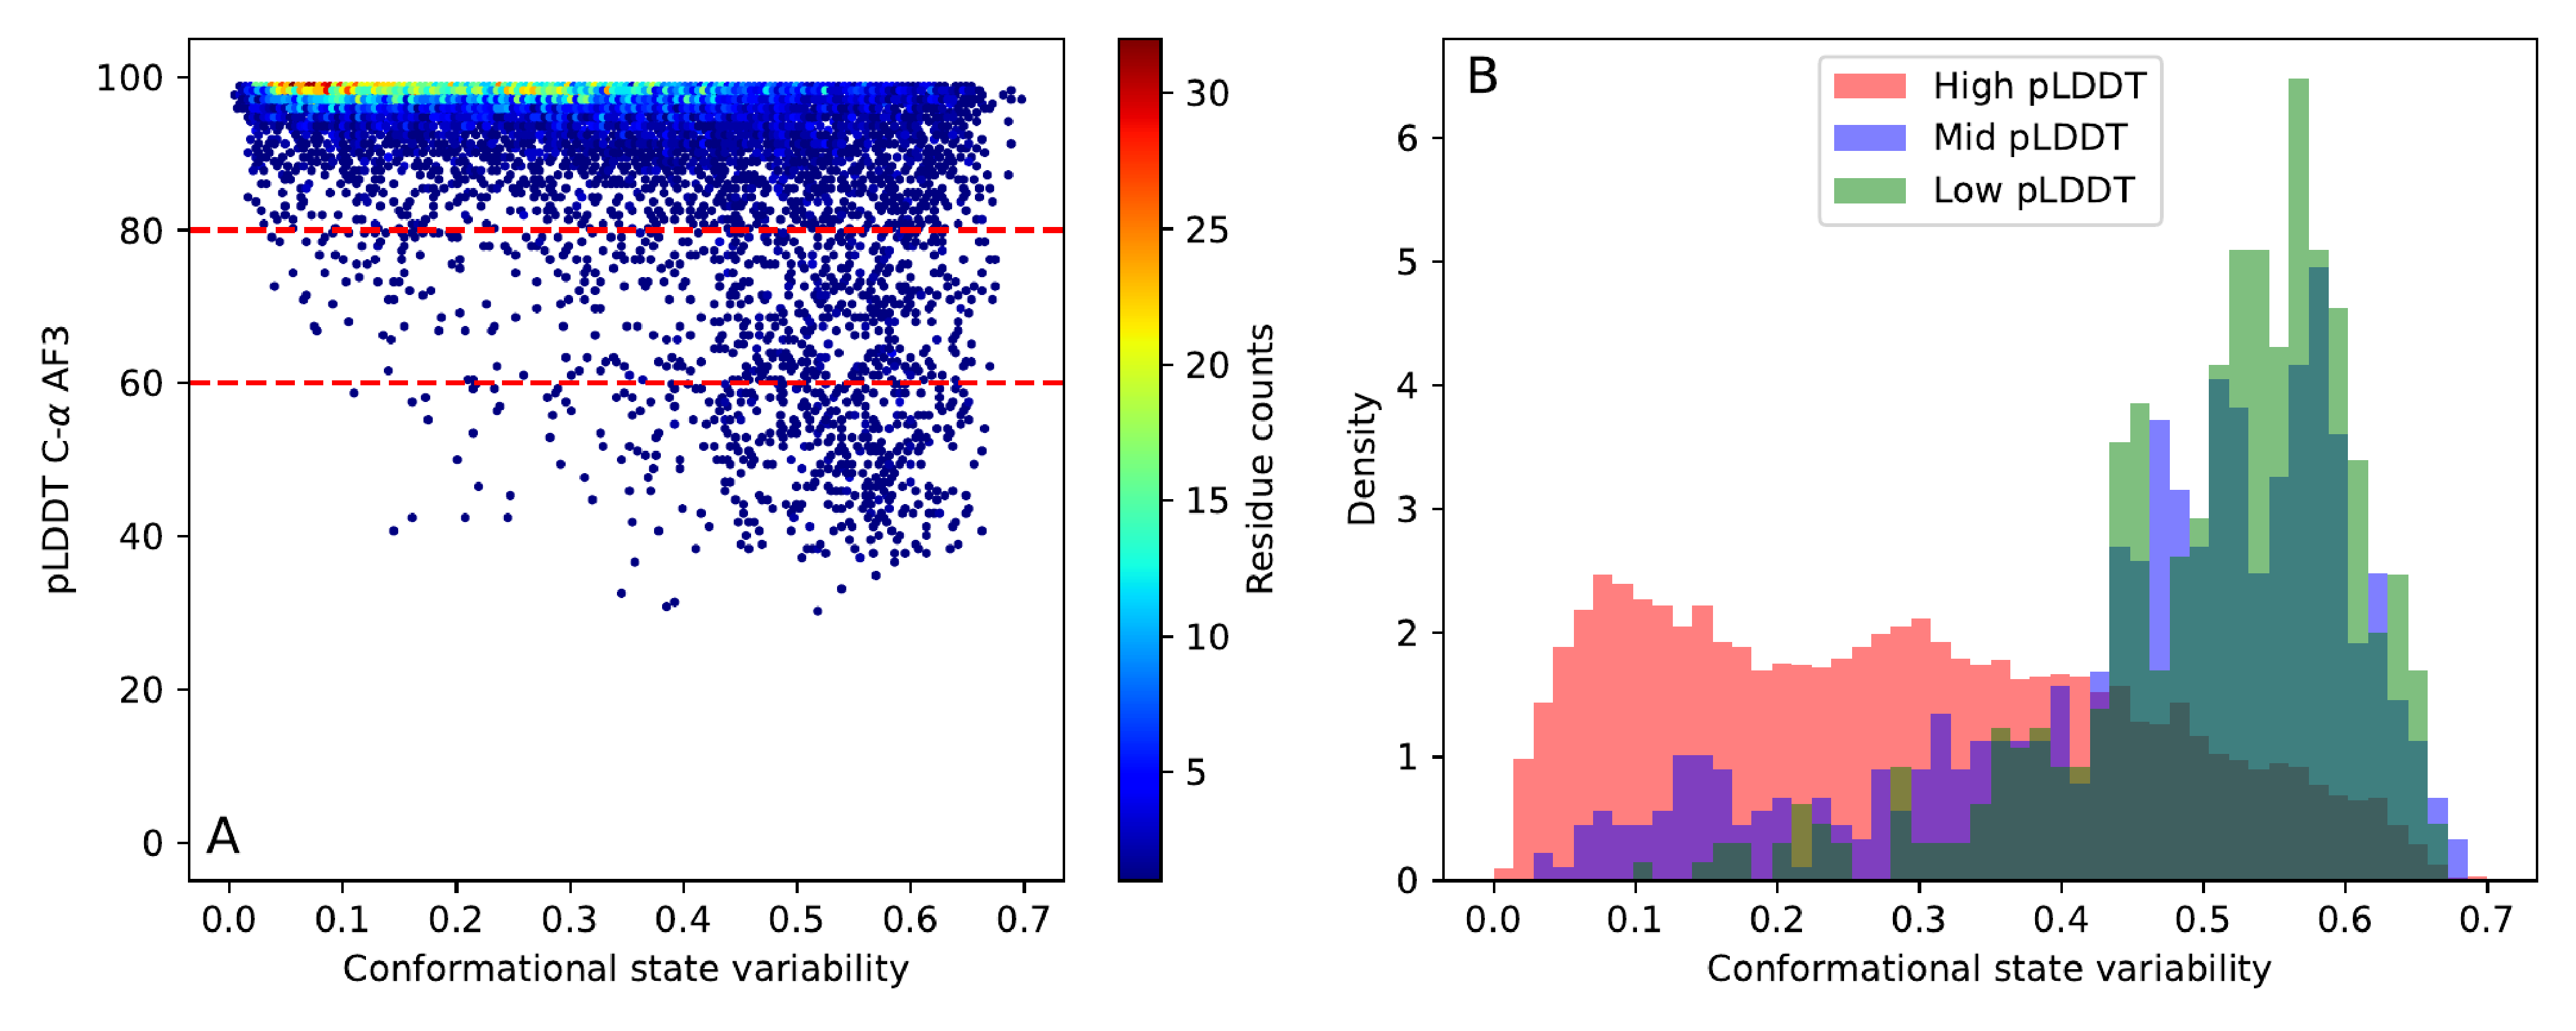
\includegraphics[width=\textwidth]{pLDDT/plddt_figures/af3_plddt_vs_conformational_state_variability_hexbin_complete_hist.pdf}
    \caption{
    \textbf{AlphaFold3 C-$\alpha$ pLDDT vs. conformational state variability.} 
    A) High pLDDT values (\( \geq 80 \), N = 10,272) concentrate in areas with lower conformational state variability. Low pLDDT \( < 60 \), N = 463) usually correspond to residues with high conformational state variability. B) This tendency is more clearly observed with pLDDT-stratified distributions, which shows that low pLDDT residues correspond to residues with high conformational state variability, therefore with high potential to exist in multiple conformations, and vice-versa for high pLDDT and low variability residues. Mid pLDDT residues \( 80 > \text{pLDDT} \geq 60 \),  N = 634) exhibit an intermediate distribution. Mann-Whitney two-sided U test yielded a p-value \( < 0.001 \) between all distributions (\supptableref{table:mann_whitney_results}). The associated distributions per propensity can be found in \suppfigref{fig:af3_plddt_vs_constava_propensities}.
    }
    \label{fig:af3_plddt_vs_conf_state_undivided}
\end{figure}


\begin{figure}[H]
    \centering
    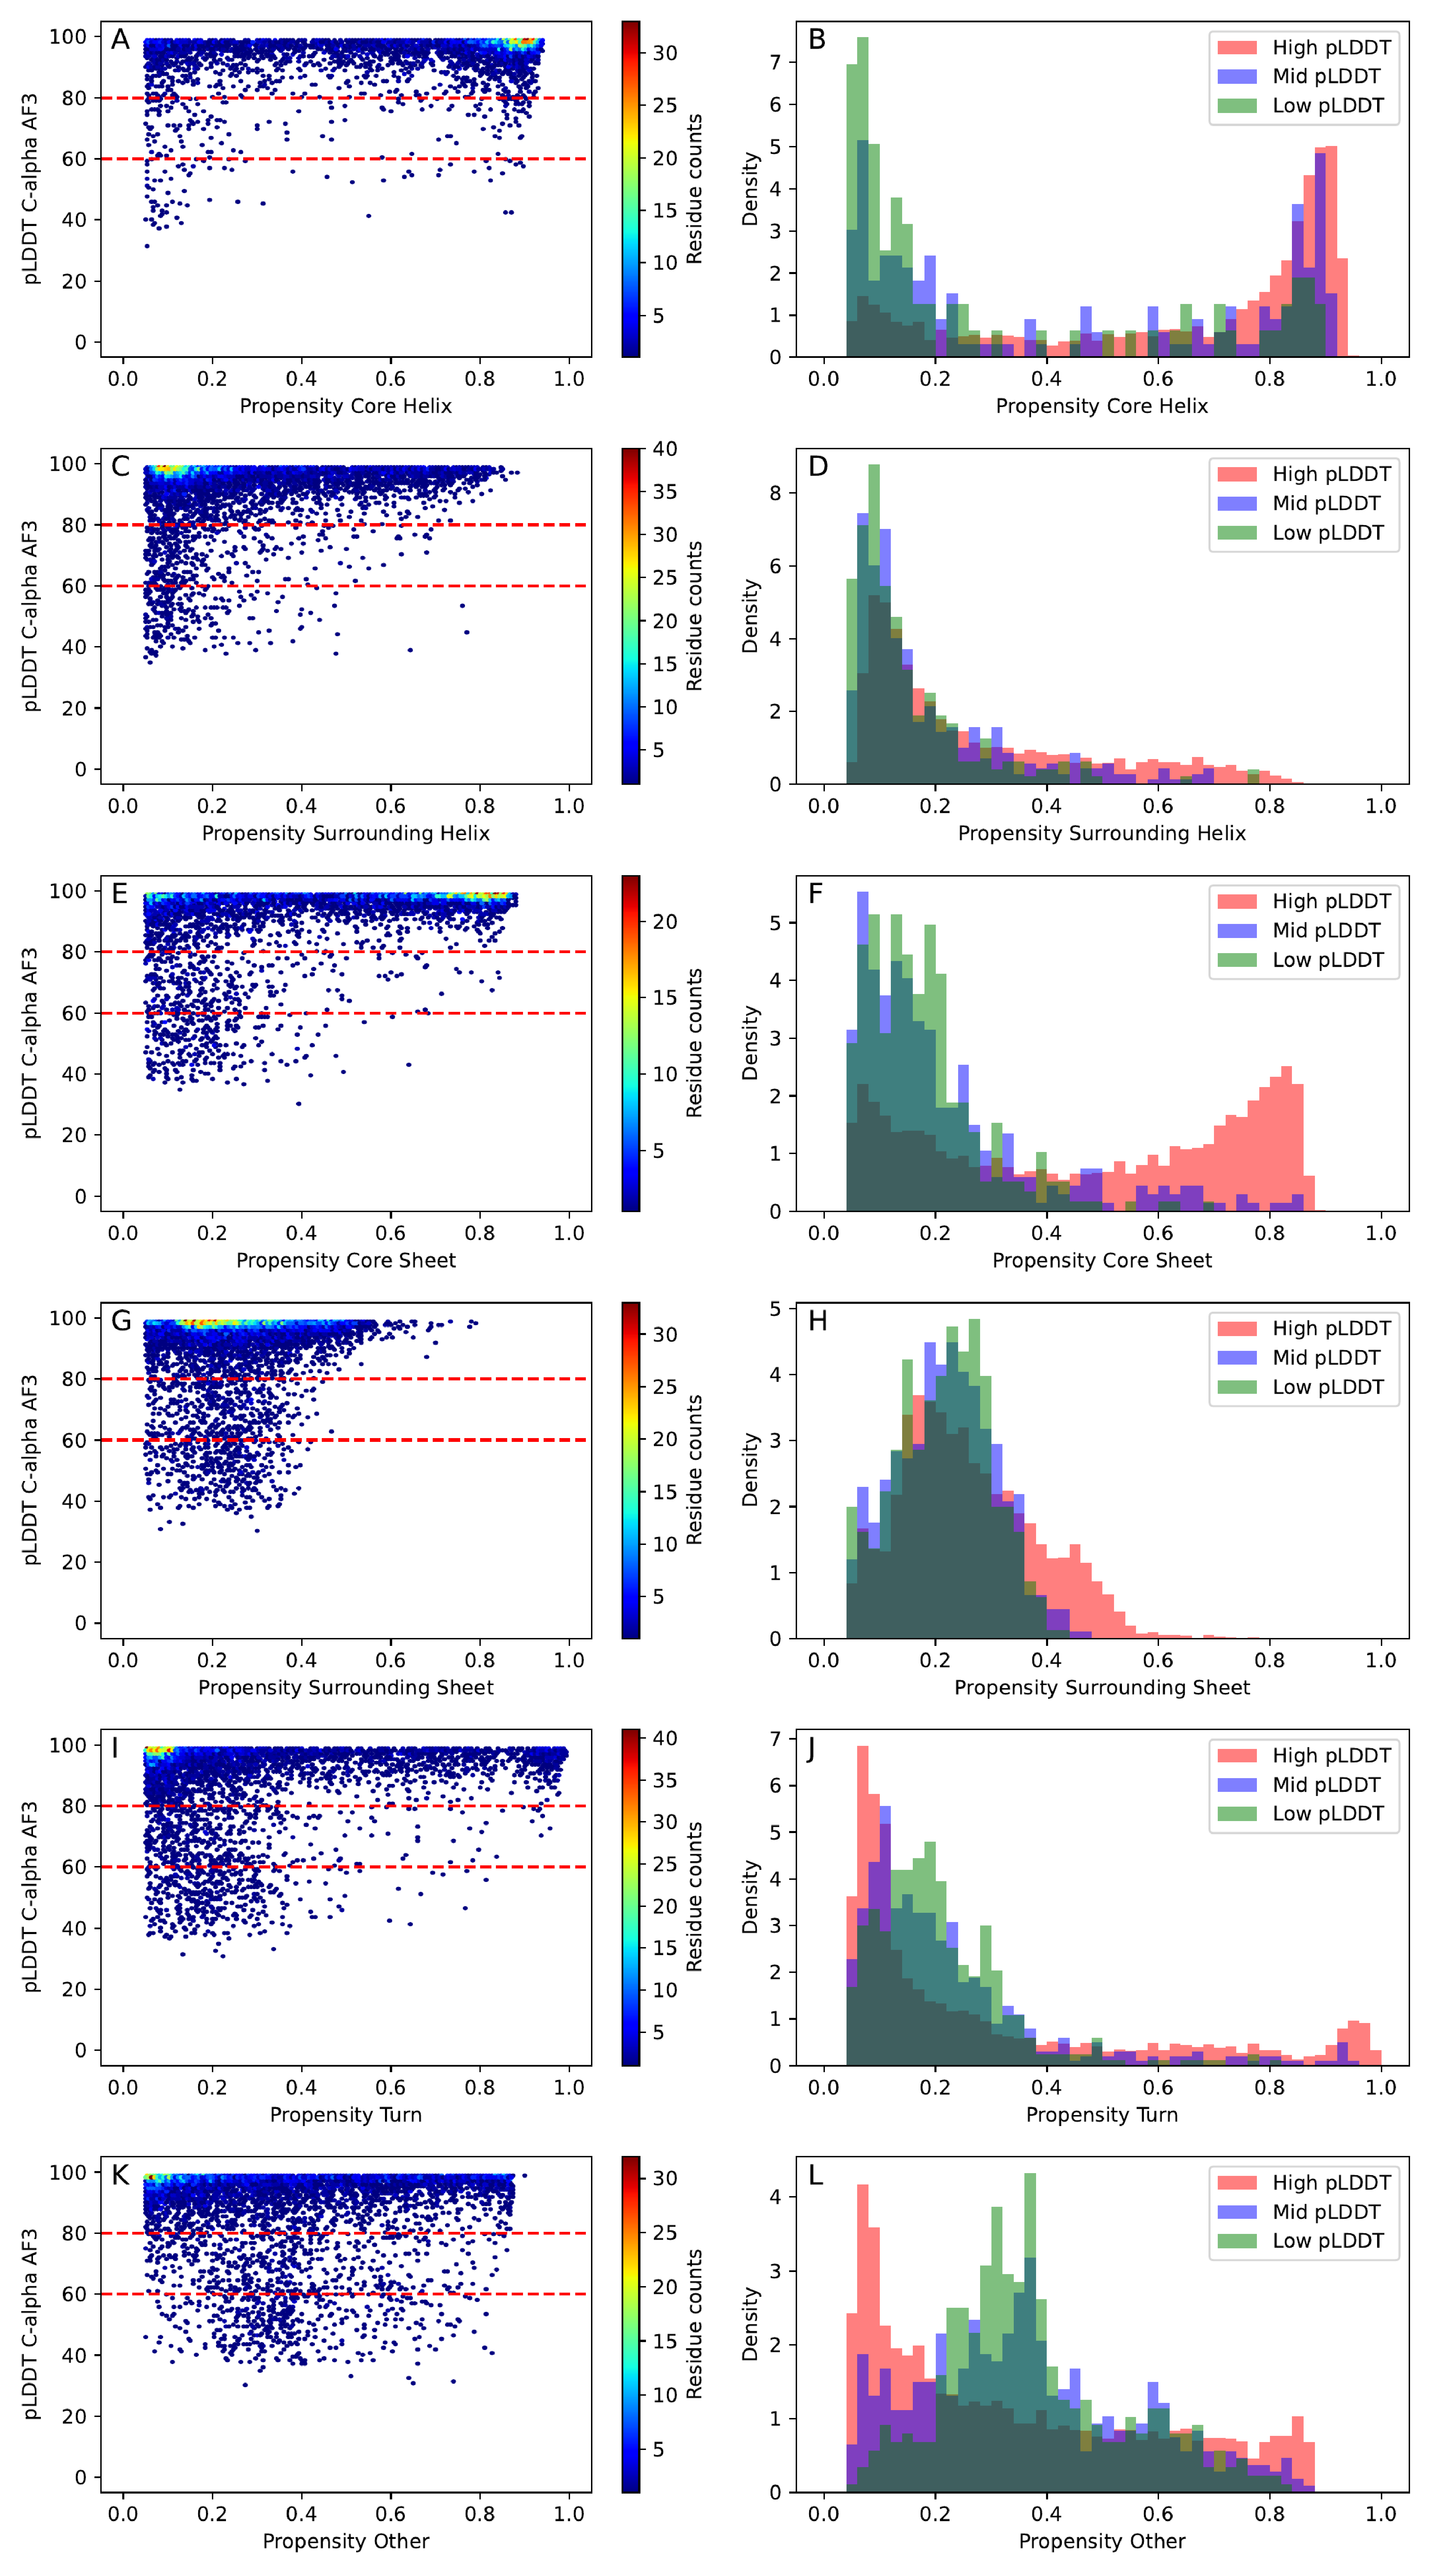
\includegraphics[width=0.83\textwidth]{pLDDT/plddt_figures/af3_plddt_vs_conformational_state_propensities_hexbin_complete_hist.pdf}
    \caption{
    \textbf{Comparison between AlphaFold3 C-$\alpha$ pLDDT and Constava's conformational state propensities.} Caption in next page.
    % The pLDDT of each residue was plotted against the propensity for each of the 6 conformational states calculated in Constava. Any propensity below 0.05 was deemed non-informative and discarded to facilitate interpretation. 
    % All residues in the MD dataset were stratified in  high (N=10,272), mid (N=634) and low (N=463) AlphaFold3 C-$\alpha$ ranges. 
    % A \& B) Hexagonal binning of AlphaFold3 C-$\alpha$ pLDDT vs Core Helix propensity and its associated pLDDT-stratified distributions. 
    % C \& D) Hexagonal binning of AlphaFold3 C-$\alpha$ pLDDT vs Surrounding Helix propensity and its associated pLDDT-stratified distributions. 
    % E \& F) Hexagonal binning of AlphaFold3 C-$\alpha$ pLDDT vs Core Sheet propensity and its associated pLDDT-stratified distributions. 
    % G \& H) Hexagonal binning of AlphaFold3 C-$\alpha$ pLDDT vs Surrounding Sheet propensity and its associated pLDDT-stratified distributions. 
    % I \& J) Hexagonal binning of AlphaFold3 C-$\alpha$ pLDDT vs Turn propensity and its associated pLDDT-stratified distributions. 
    % K \& L) Hexagonal binning of AlphaFold3 C-$\alpha$ pLDDT vs Other propensity and its associated pLDDT-stratified distributions. 
    % The p-values for the Mann-Whitney two-sided U tests between each pLDDT-stratified distribution for every conformational state can be found in supplementary table \ref{table:mann_whitney_results_md}.
    }
\label{fig:af3_plddt_vs_constava_propensities}
\end{figure}

\begin{figure}[H]
  \ContinuedFloat
  \caption[]{ (Continuation) The pLDDT of each residue was plotted against the propensity for each of the 6 conformational states calculated in Constava. Any propensity below 0.05 was deemed non-informative and discarded to facilitate interpretation. 
    All residues in the MD dataset were stratified in  high (N=10,272), mid (N=634) and low (N=463) AlphaFold3 C-$\alpha$ ranges. 
    A \& B) Hexagonal binning of AlphaFold3 C-$\alpha$ pLDDT vs Core Helix propensity and its associated pLDDT-stratified distributions. 
    C \& D) Hexagonal binning of AlphaFold3 C-$\alpha$ pLDDT vs Surrounding Helix propensity and its associated pLDDT-stratified distributions. 
    E \& F) Hexagonal binning of AlphaFold3 C-$\alpha$ pLDDT vs Core Sheet propensity and its associated pLDDT-stratified distributions. 
    G \& H) Hexagonal binning of AlphaFold3 C-$\alpha$ pLDDT vs Surrounding Sheet propensity and its associated pLDDT-stratified distributions. 
    I \& J) Hexagonal binning of AlphaFold3 C-$\alpha$ pLDDT vs Turn propensity and its associated pLDDT-stratified distributions. 
    K \& L) Hexagonal binning of AlphaFold3 C-$\alpha$ pLDDT vs Other propensity and its associated pLDDT-stratified distributions. 
    The p-values for the Mann-Whitney two-sided U tests between each pLDDT-stratified distribution for every conformational state can be found in \supptableref{table:mann_whitney_results_md}.}
\end{figure}


\begin{figure}[H]
    \centering
    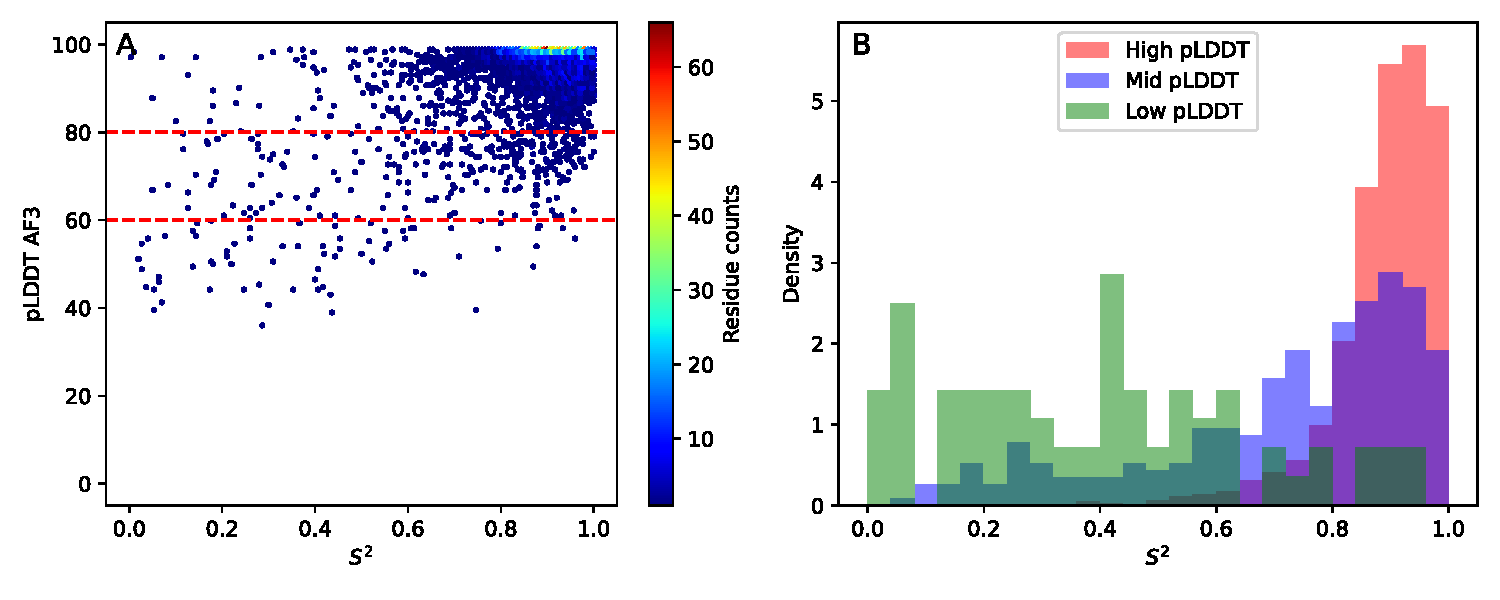
\includegraphics[width=\textwidth]{pLDDT/plddt_figures/s2_vs_plddt_af3_hexbin_undivided_hist.pdf}
    \caption{\textbf{Comparison between AlphaFold3 C-$\alpha$ pLDDT and \(S^{2}\).} Most residues in this dataset exhibit high pLDDT and high \(S^{2}\) values, represented by warmer hues in panel A. Due to the limited and uneven residues sample sizes (high pLDDT, \( \geq 80 \), N = 4,125; mid pLDDT, \( 80 > \text{pLDDT} \geq 60 \),  N = 287; low pLDDT, \( < 60 \), N = 70), it is challenging to make definitive conclusions about the sparsely populated mid and low pLDDT regions. Panel B illustrates the distributions of \(S^{2}\) values of each pLDDT range, for which Mann-Whitney two-sided U test yielded a p-value \( < 0.001 \) between all distributions (\supptableref{table:mann_whitney_results}).}

    \label{fig:af3_plddt_vs_s2_undivided}
\end{figure}

\begin{figure}[H]
    \centering
    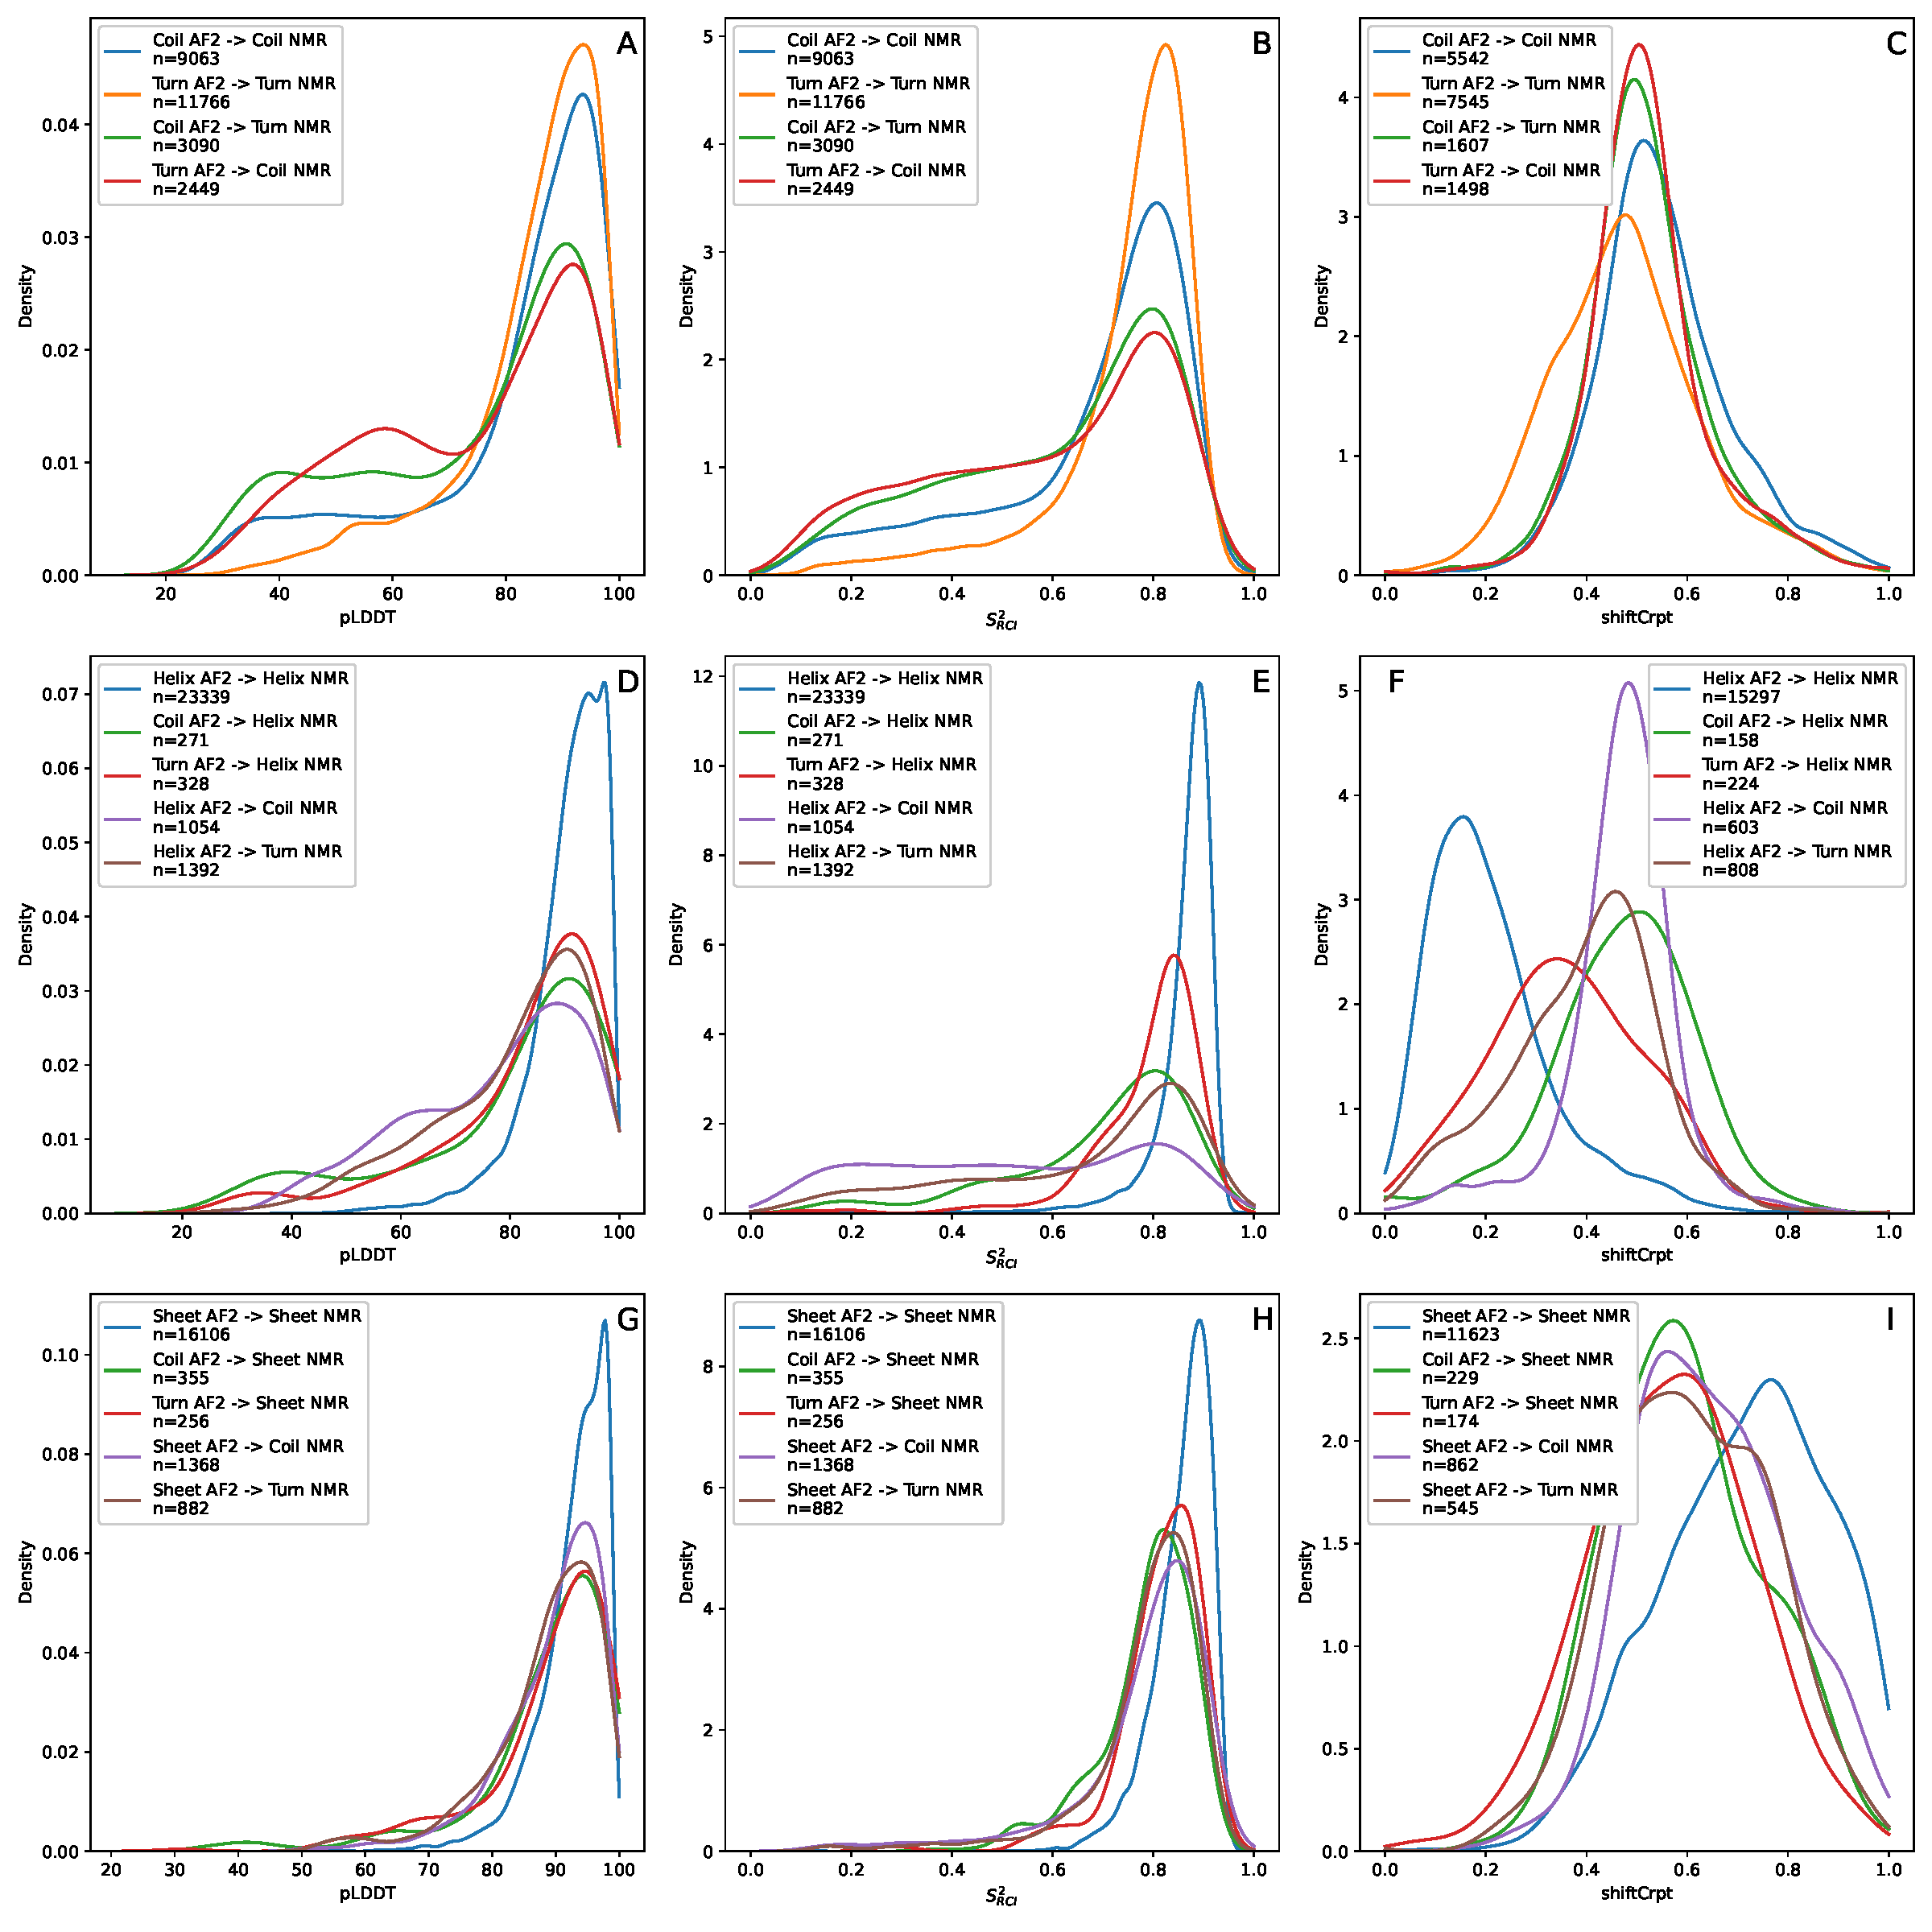
\includegraphics[width=\textwidth]{pLDDT/plddt_figures/all_switchers_ss_af_stride_consensus_af_stride_af_ss_nmr_strideCons.pdf}
        \caption{\textbf{Distribution of STRIDE fold assignment matches and mismatches between AlphaFold2 structures and consensus NMR ensemble assignments, for diverse metrics.} Those residues in the \(S^{2}_{RCI}\) dataset with STRIDE consensus were stratified according to their secondary assignment pairs, derived from AlphaFold2 structures and the NMR models consensus assignment. A, D \& G) pLDDT distributions for residues whose consensus STRIDE assignment from NMR ensembles and from AlphaFold2 models match or mismatch. B, E \& H) \(S^{2}_{RCI}\) distributions for residues whose consensus STRIDE assignment from NMR ensembles and from AlphaFold2 models match or mismatch. C, F \& I) shiftCrypt distributions for residues whose consensus STRIDE assignment from NMR ensembles and from AlphaFold2 models match or mismatch.}
    \label{fig:af2_nmr_fold_missmatch}
\end{figure}


\begin{figure}[H]
    \centering
    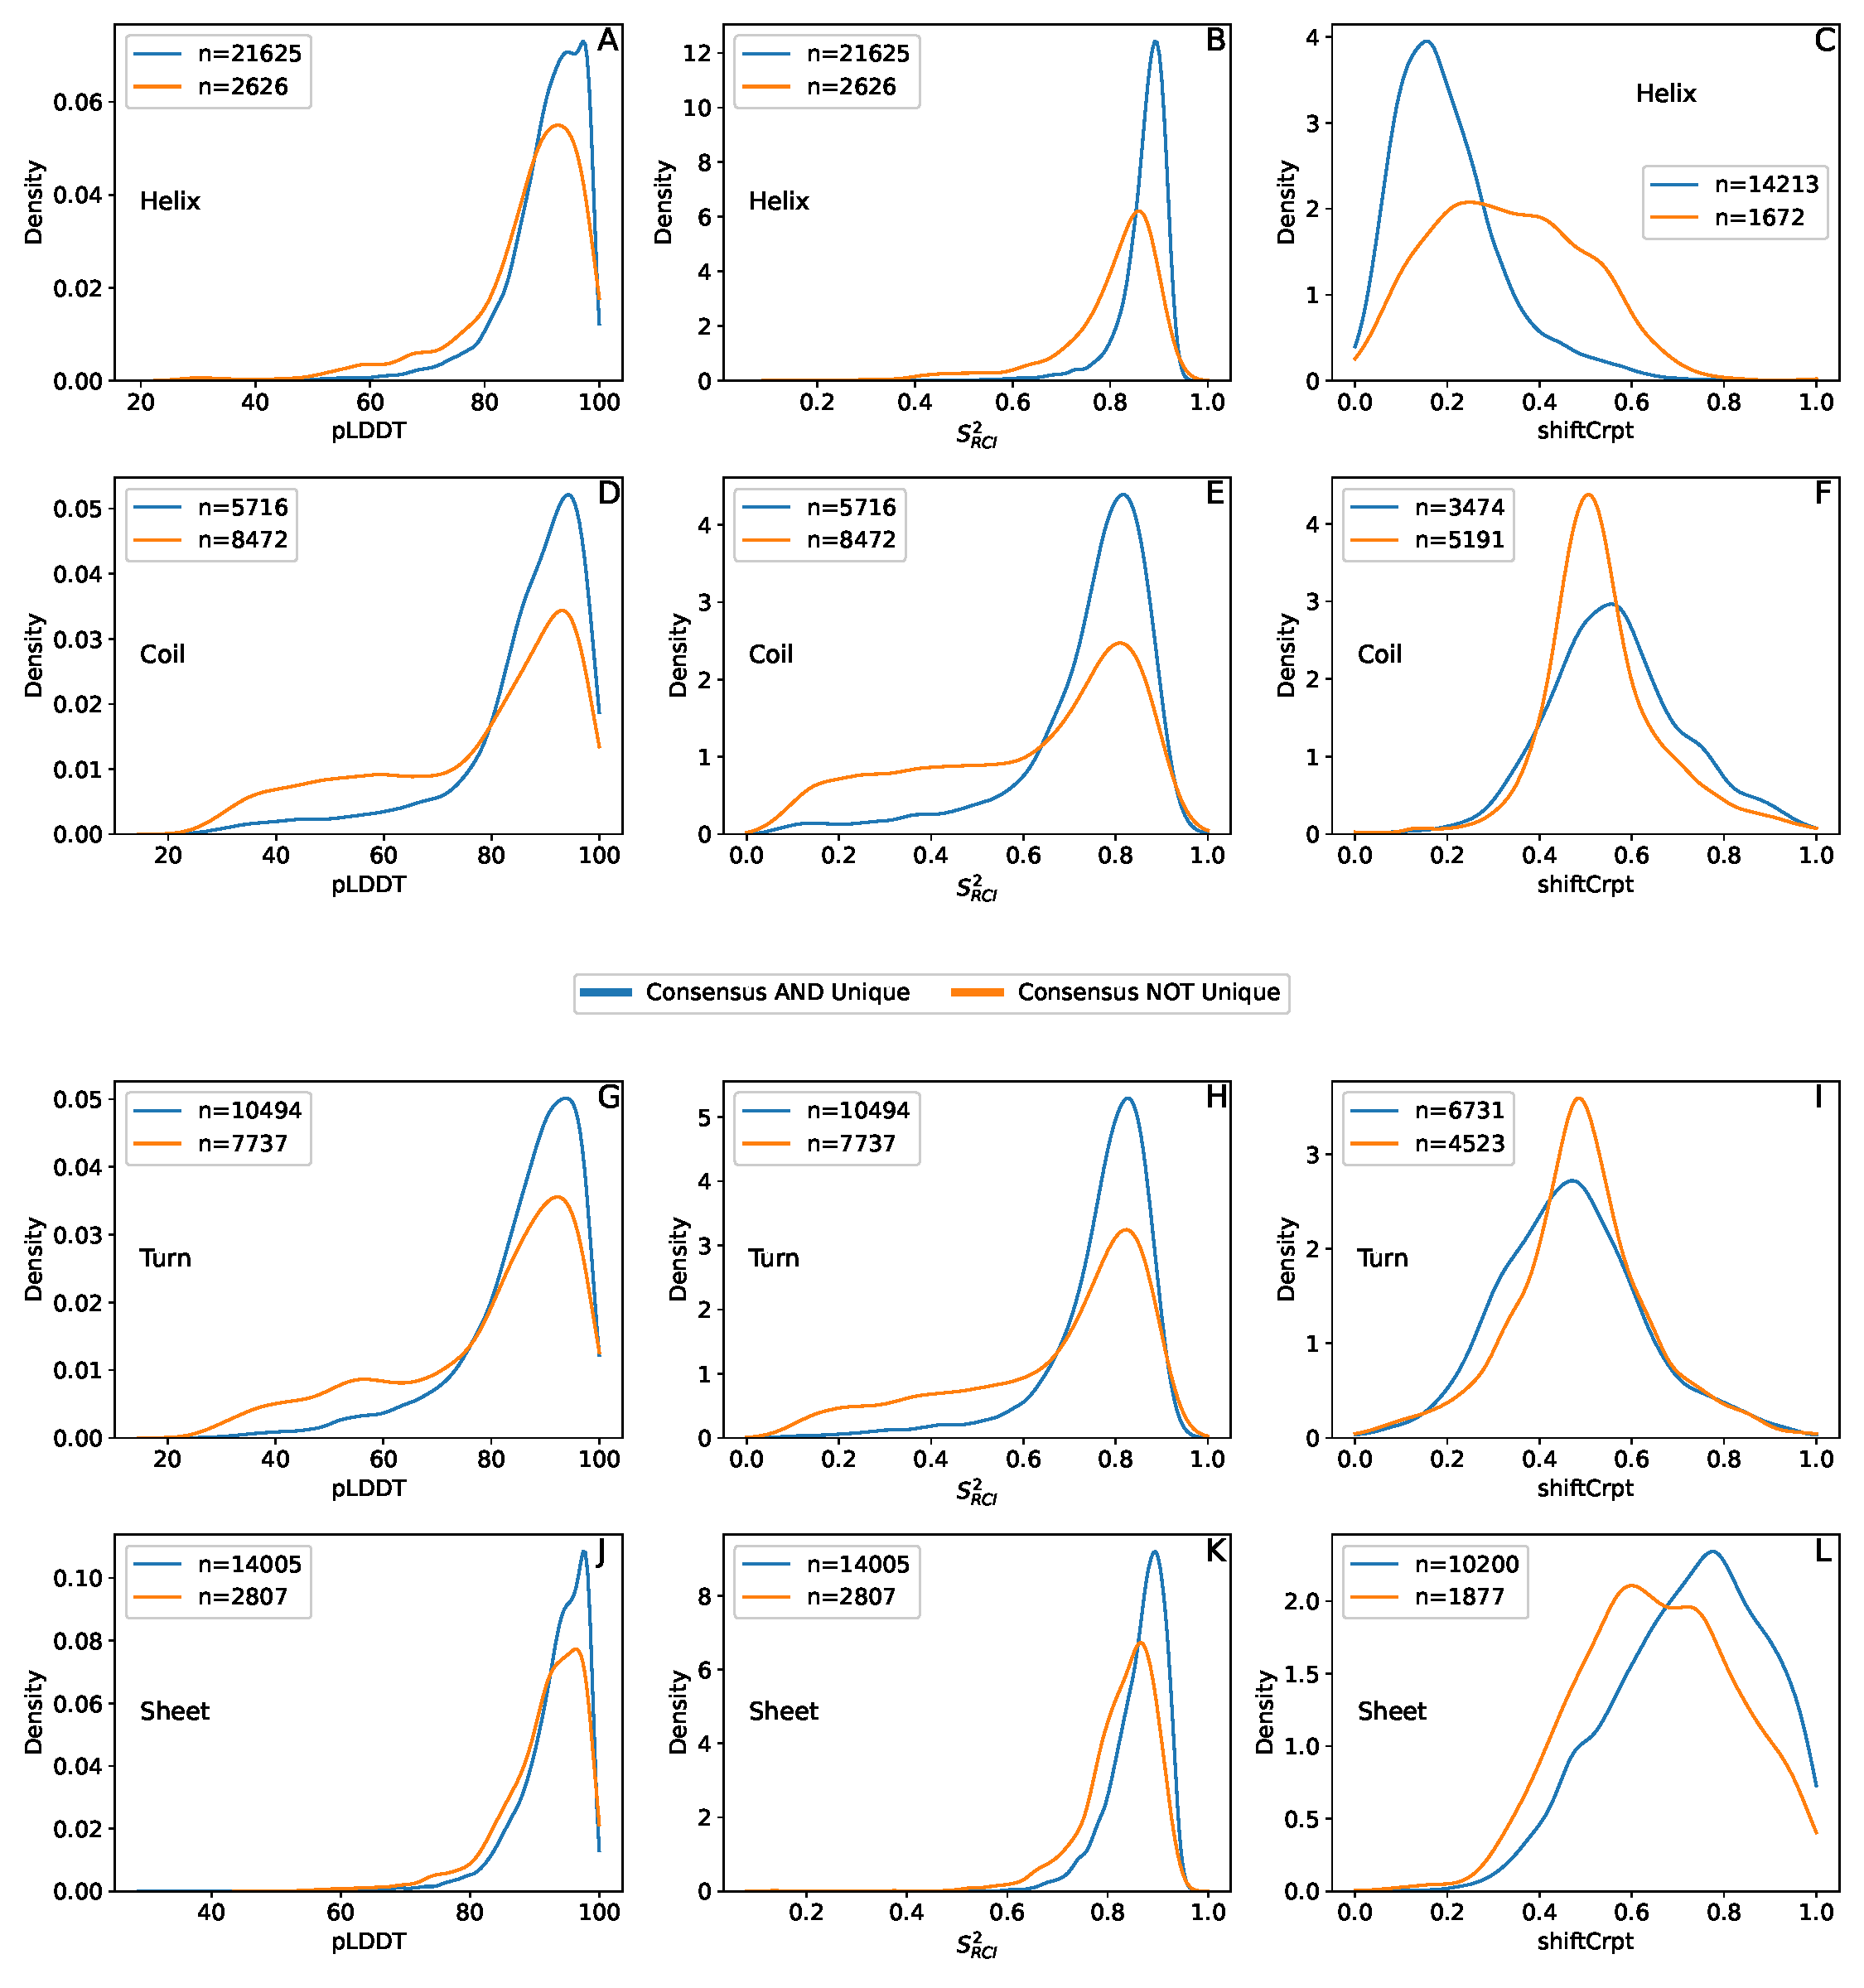
\includegraphics[width=\textwidth]{pLDDT/plddt_figures/with_and_without_unique_nmr_strideCons_stratified.pdf}
    \caption{\textbf{Distribution of residues with  NMR consensus STRIDE assignment with and without unique STRIDE assignment, for diverse metrics.} Those residues in the \(S^{2}_{RCI}\) dataset with STRIDE consensus were stratified according to whether they featured a unique STRIDE assignment across all the models in their corresponding NMR ensemble. A, D, G \& J) pLDDT distributions for $\alpha$-helix, coil, turn and $\beta$-sheet respectively. B, E, H \& K) \(S^{2}_{RCI}\) distributions for $\alpha$-helix, coil, turn and $\beta$-sheet respectively. C, F, I \& L) shiftCrypt distributions for $\alpha$-helix, coil, turn and $\beta$-sheet respectively.}

    \label{fig:unique_and_or_cons}
\end{figure}

\begin{figure}[H]
    \centering
    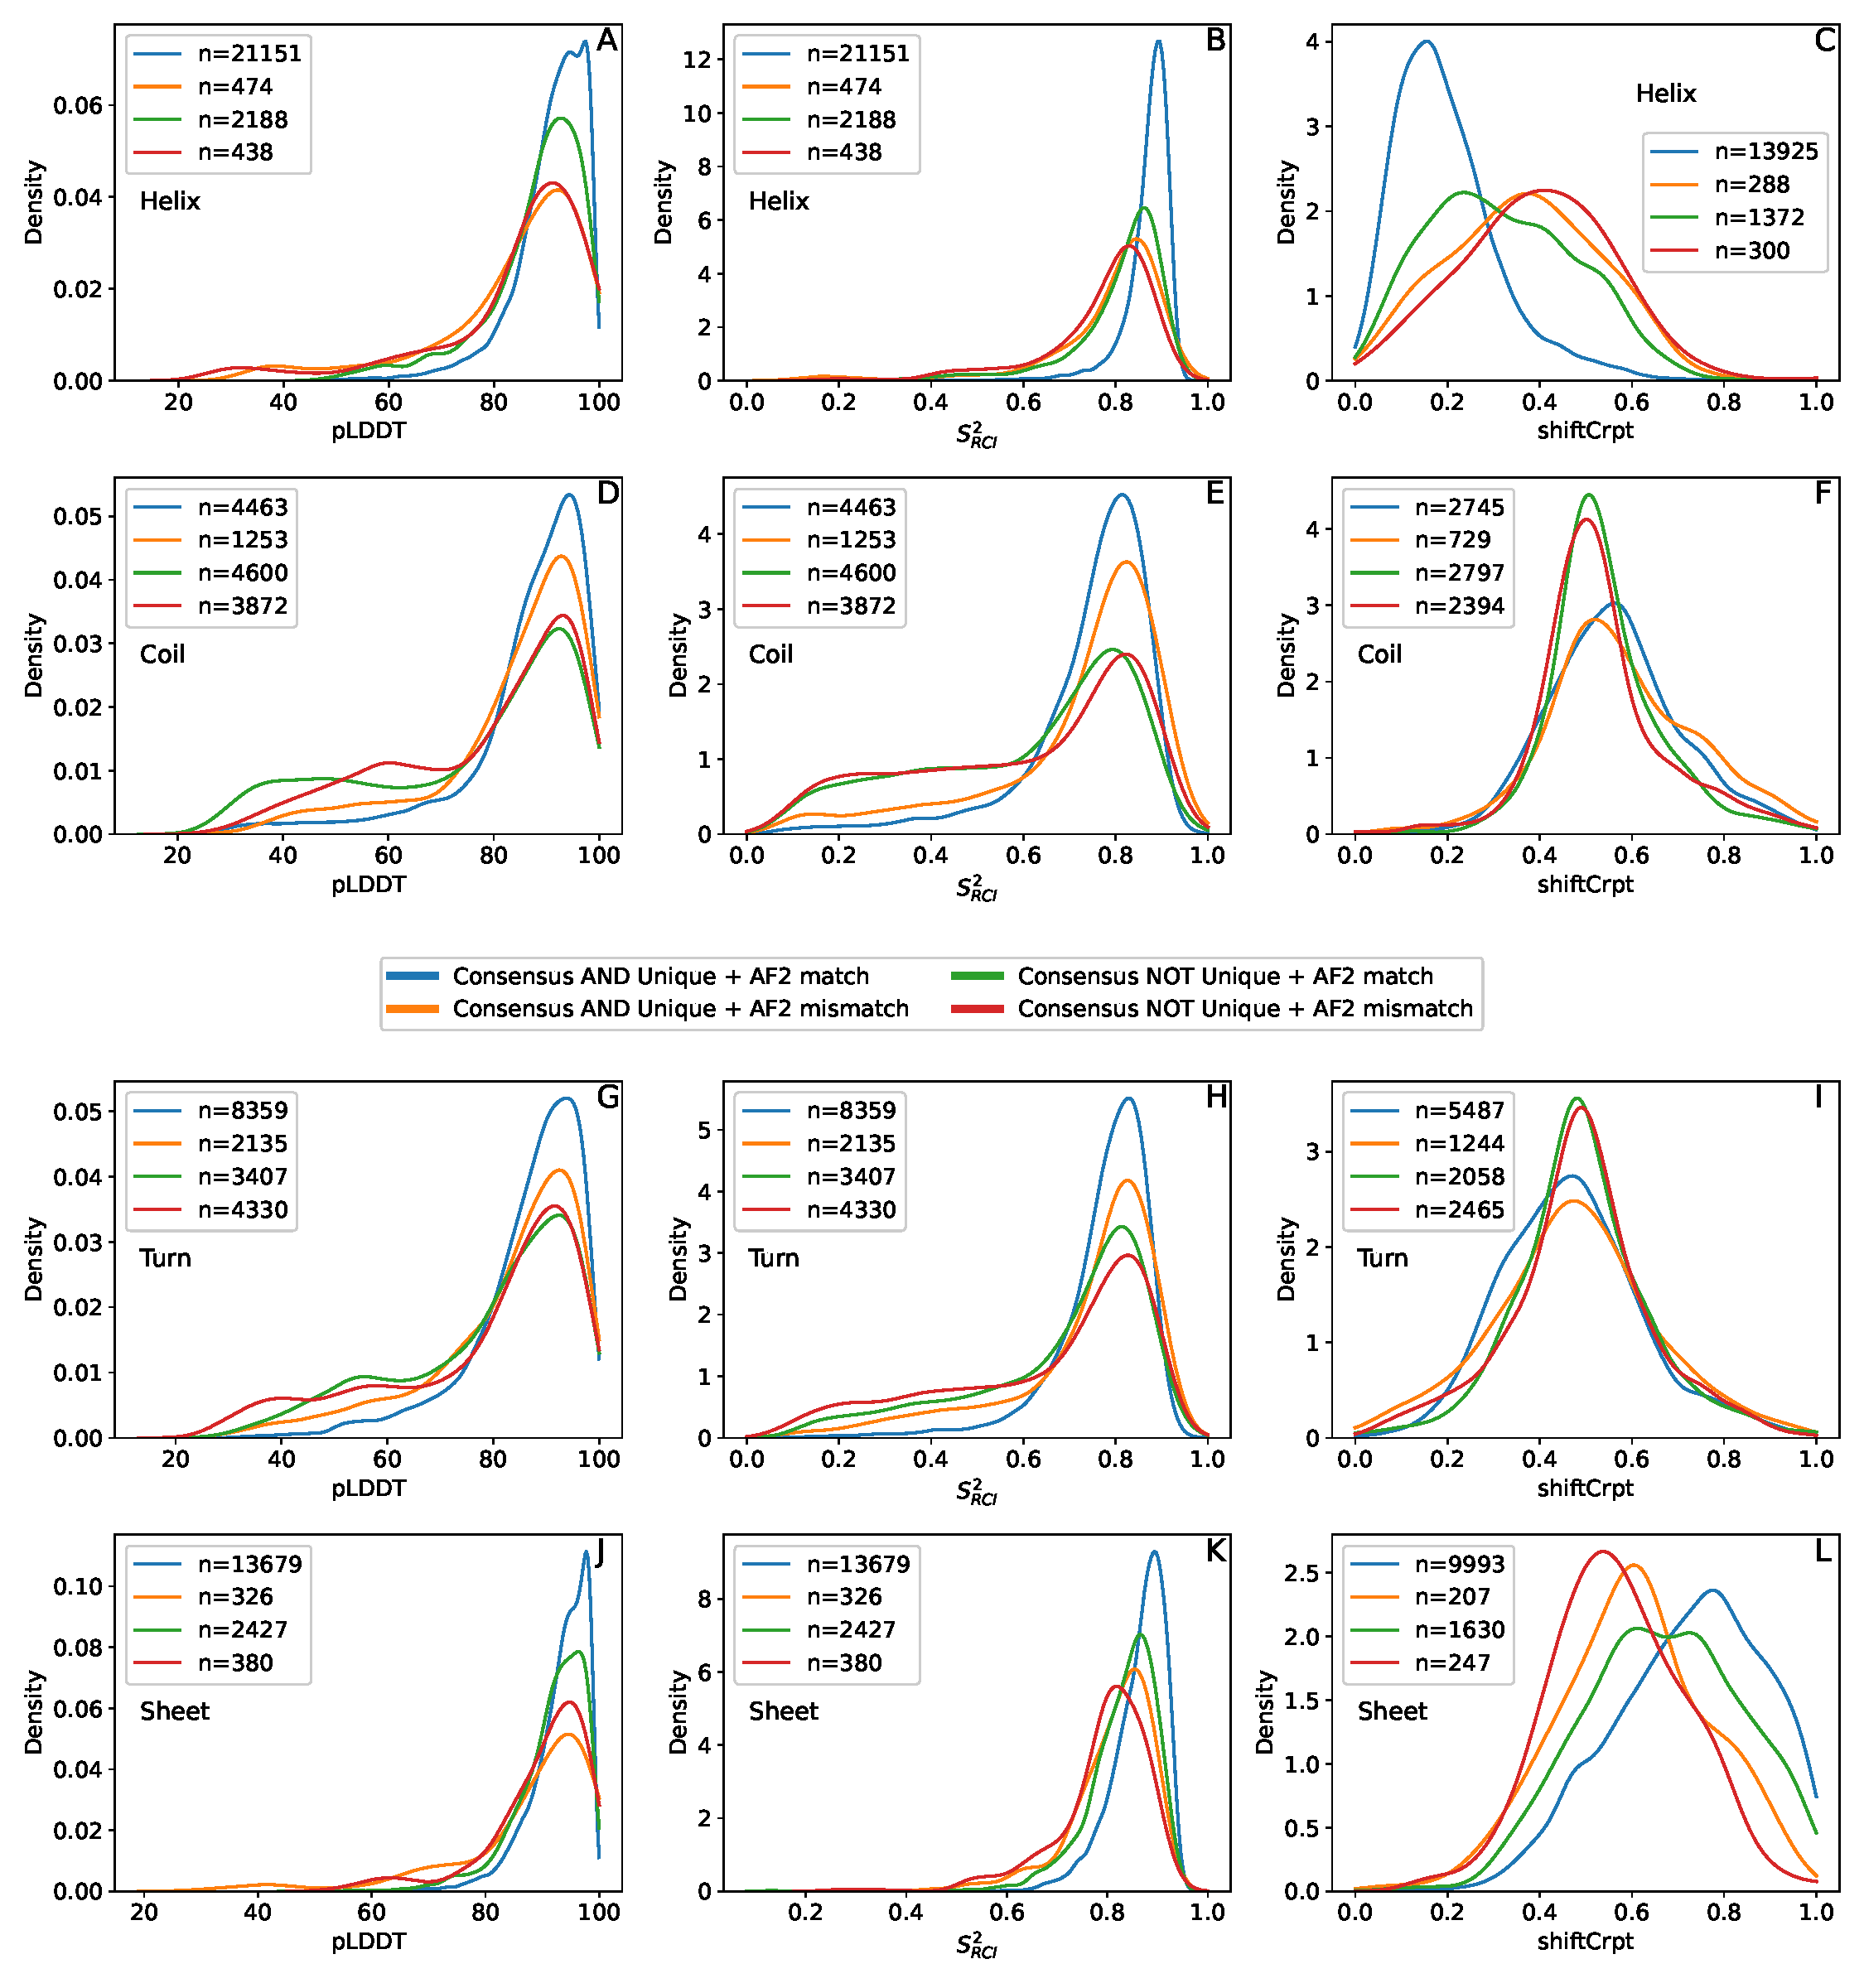
\includegraphics[width=\textwidth]{pLDDT/plddt_figures/with_and_without_unique_nmr_strideCons_stratified_match_mismatch.pdf}
    \caption{\textbf{Distribution of residues with  NMR consensus STRIDE assignment with and without unique STRIDE assignment, with matching and mismatching NMR and AlphaFold2 fold assignments, for diverse metrics.} Those residues in the \(S^{2}_{RCI}\) dataset with STRIDE consensus were stratified according to whether they featured a unique STRIDE assignment across all the models in their corresponding NMR ensemble. Then, they were further stratified on whether or not their NMR consensus STRIDE assignment matched the AlphaFold2 STRIDE assignment. A, D, G \& J) pLDDT distributions for $\alpha$-helix, coil, turn and $\beta$-sheet respectively. B, E, H \& K) \(S^{2}_{RCI}\) distributions for $\alpha$-helix, coil, turn and $\beta$-sheet respectively. C, F, I \& L) shiftCrypt distributions for $\alpha$-helix, coil, turn and $\beta$-sheet respectively.}

    \label{fig:unique_and_or_cons_match_af2}
\end{figure}

\begin{table}[H]
	\centering
 \footnotesize
 \caption{\textbf{Results of the Mann-Whitney two-sided U tests between pLDDT-stratified subsets per Constava's conformational states on the MD dataset.} For each of Constava's conformational states, the pLDDT-stratified subsets were tested against each other with a Mann-Whitney two-sided U test to assess differential distributions.}
\begin{tabular}{@{}ccccr@{}}
\toprule
\begin{tabular}[c]{@{}c@{}}Conformational\\ state\end{tabular} &
  \begin{tabular}[c]{@{}c@{}}AlphaFold\\ version\end{tabular} &
  \begin{tabular}[c]{@{}c@{}}pLDDT\\ ranges\end{tabular} &
  \begin{tabular}[c]{@{}c@{}}Difference \\ between means\end{tabular} &
  \multicolumn{1}{c}{p-value} \\ \midrule
Core Helix  & 2 & High-Mid & 0.2161  & 6.67 x 10\(^{\text{-34}}\)  \\
Core Helix  & 2 & High-Low & 0.3427  & 2.52 x 10\(^{\text{-31}}\)  \\
Core Helix  & 2 & Mid-Low  & 0.1266  & 1.53 x 10\(^{\text{-5}}\)   \\ 
\arrayrulecolor[gray]{0.8}\hline
Surr. Helix & 2 & High-Mid & 0.0264  & 0.01955                   \\
Surr. Helix & 2 & High-Low & 0.1168  & 5.17 x 10\(^{\text{-43}}\)  \\
Surr. Helix & 2 & Mid-Low  & 0.0903  & 1.24 x 10\(^{\text{-20}}\)  \\
\arrayrulecolor[gray]{0.8}\hline
Core Sheet  & 2 & High-Mid & 0.2254  & 1.60 x 10\(^{\text{-60}}\)  \\
Core Sheet  & 2 & High-Low & 0.3074  & 2.12 x 10\(^{\text{-104}}\) \\
Core Sheet  & 2 & Mid-Low  & 0.0821  & 1.58 x 10\(^{\text{-5}}\)   \\
\arrayrulecolor[gray]{0.8}\hline
Surr. Sheet & 2 & High-Mid & 0.0339  & 1.96 x 10\(^{\text{-8}}\)   \\
Surr. Sheet & 2 & High-Low & 0.0455  & 3.02 x 10\(^{\text{-15}}\)  \\
Surr. Sheet & 2 & Mid-Low  & 0.0117  & 0.08711                   \\
\arrayrulecolor[gray]{0.8}\hline
Turn        & 2 & High-Mid & 0.0394  & 0.44796                   \\
Turn        & 2 & High-Low & 0.0826  & 0.22141                   \\
Turn        & 2 & Mid-Low  & 0.0432  & 0.45743                   \\
\arrayrulecolor[gray]{0.8}\hline
Other       & 2 & High-Mid & 0.0082  & 0.28323                   \\
Other       & 2 & High-Low & -0.0397 & 6.19 x 10\(^{\text{-15}}\)  \\
Other       & 2 & Mid-Low  & -0.0479 & 1.85 x 10\(^{\text{-9}}\)   \\
\arrayrulecolor[gray]{0.8}\hline
Core Helix  & 3 & High-Mid & 0.1990  & 4.07 x 10\(^{\text{-14}}\)  \\
Core Helix  & 3 & High-Low & 0.3498  & 4.63 x 10\(^{\text{-20}}\)  \\
Core Helix  & 3 & Mid-Low  & 0.1507  & 1.85 x 10\(^{\text{-4}}\)   \\
\arrayrulecolor[gray]{0.8}\hline
Surr. Helix & 3 & High-Mid & 0.0861  & 6.18 x 10\(^{\text{-18}}\)  \\
Surr. Helix & 3 & High-Low & 0.1203  & 7.55 x 10\(^{\text{-27}}\)  \\
Surr. Helix & 3 & Mid-Low  & 0.0343  & 0.00256                   \\
\arrayrulecolor[gray]{0.8}\hline
Core Sheet  & 3 & High-Mid & 0.2657  & 1.94 x 10\(^{\text{-58}}\)  \\
Core Sheet  & 3 & High-Low & 0.3019  & 6.68 x 10\(^{\text{-64}}\)  \\
Core Sheet  & 3 & Mid-Low  & 0.0362  & 0.29869                   \\
\arrayrulecolor[gray]{0.8}\hline
Surr. Sheet & 3 & High-Mid & 0.0423  & 6.90 x 10\(^{\text{-10}}\)  \\
Surr. Sheet & 3 & High-Low & 0.0462  & 1.51 x 10\(^{\text{-10}}\)  \\
Surr. Sheet & 3 & Mid-Low  & 0.0039  & 0.66095                   \\
\arrayrulecolor[gray]{0.8}\hline
Turn        & 3 & High-Mid & 0.0628  & 0.48281                   \\
Turn        & 3 & High-Low & 0.0779  & 0.13434                   \\
Turn        & 3 & Mid-Low  & 0.0152  & 0.33197                   \\
\arrayrulecolor[gray]{0.8}\hline
Other       & 3 & High-Mid & -0.0178 & 0.000078                  \\
Other       & 3 & High-Low & -0.0288 & 2.72 x 10\(^{\text{-8}}\)   \\
Other       & 3 & Mid-Low  & -0.0110 & 0.15908                   \\ \arrayrulecolor{black} \bottomrule
\end{tabular}
	\label{table:mann_whitney_results_md}
\end{table}

\begin{table}[H]
\centering
\small
\caption{\textbf{Results of the Mann-Whitney two-sided U tests between pLDDT-stratified subsets for $S^{2}_{RCI}$ $\delta 2D$ conformations in AlphaFold2.} For each conformation type, the pLDDT-stratified subsets were tested against each other with a Mann-Whitney two-sided U test to assess differential distributions. \textit{Note: p-values marked with * were too low for Scipy to differentiate from 0.}}
\begin{tabular}{@{}cccr@{}}
\toprule
Conformation & \begin{tabular}[c]{@{}c@{}}pLDDT\\ ranges\end{tabular} & \begin{tabular}[c]{@{}c@{}}Difference\\ between means\end{tabular} & \multicolumn{1}{c}{p-value} \\ \midrule
$\delta 2D$ Helix & High-Mid & 0.1185  & 3.38 x 10\(^{\text{-55}}\)  \\
$\delta 2D$ Helix & High-Low & 0.2896  & 0.0*                      \\
$\delta 2D$ Helix & Mid-Low  & 0.1711  & 1.23 x 10\(^{\text{-300}}\) \\
\arrayrulecolor[gray]{0.8}\hline
$\delta 2D$ Sheet & High-Mid & 0.1181  & 5.03 x 10\(^{\text{-49}}\)  \\
$\delta 2D$ Sheet & High-Low & 0.1723  & 5.44 x 10\(^{\text{-53}}\)  \\
$\delta 2D$ Sheet & Mid-Low  & 0.0542  & 2.63 x 10\(^{\text{-7}}\)   \\
\arrayrulecolor[gray]{0.8}\hline
$\delta 2D$ Coil  & High-Mid & -0.1775 & 0.0*                      \\
$\delta 2D$ Coil  & High-Low & -0.3184 & 0.0*                      \\
$\delta 2D$ Coil  & Mid-Low  & -0.1410 & 3.76 x 10\(^{\text{-305}}\) \\
\arrayrulecolor[gray]{0.8}\hline
$\delta 2D$ PPII  & High-Mid & -0.0592 & 0.0*                      \\
$\delta 2D$ PPII  & High-Low & -0.1435 & 0.0*                      \\
$\delta 2D$ PPII  & Mid-Low  & -0.0843 & 0.0*                      \\ \arrayrulecolor{black} \bottomrule
\end{tabular}

\label{table:mann_whitney_results_delta2d}
\end{table}


\begin{table}[H]
\centering
\small
\caption{\textbf{Results of the Mann-Whitney two-sided U tests between pLDDT-stratified subsets.} For each dataset, the pLDDT-stratified subsets were tested against each other with a Mann-Whitney two-sided U test to assess differential distributions. \textit{Note: p-values marked with * were too low for Scipy to differentiate from 0.}}
\begin{tabular}{@{}cccccr@{}}
\toprule
Dataset &
  Metric &
  \begin{tabular}[c]{@{}c@{}}AlphaFold\\ version\end{tabular} &
  \begin{tabular}[c]{@{}c@{}}pLDDT\\ ranges\end{tabular} &
  \begin{tabular}[c]{@{}c@{}}Difference\\ between \\means\end{tabular} &
  \multicolumn{1}{c}{p-value} \\ \midrule
\(S^{2}_{\text{RCI}}\) & \(S^{2}_{\text{RCI}}\)  & 2 & high-mid & 0.1417  & 0*                        \\
\(S^{2}_{\text{RCI}}\) & \(S^{2}_{\text{RCI}}\)  & 2 & high-low & 0.4150  & 0*                        \\
\(S^{2}_{\text{RCI}}\) & \(S^{2}_{\text{RCI}}\)  & 2 & mid-low  & 0.2732  & 0*                        \\ \arrayrulecolor[gray]{0.8}\hline
\(S^{2}_{\text{RCI}}\) & ShiftCrypt            & 2 & high-mid & 0.0152  & 0.002                     \\
\(S^{2}_{\text{RCI}}\) & ShiftCrypt            & 2 & high-low & -0.0201 & 4.55 x 10\(^{\text{-7}}\)   \\
\(S^{2}_{\text{RCI}}\) & ShiftCrypt            & 2 & mid-low  & -0.0353 & 9.45 x 10\(^{\text{-21}}\)  \\ \arrayrulecolor[gray]{0.8}\hline
\(S^{2}_{\text{RCI}}\) & \begin{tabular}[c]{@{}c@{}}Solvent\\accessibility\end{tabular} & 2 & high-mid & -0.1851 & 0*                        \\
\(S^{2}_{\text{RCI}}\) & \begin{tabular}[c]{@{}c@{}}Solvent\\accessibility\end{tabular} & 2 & high-low & -0.3521 & 0*                        \\
\(S^{2}_{\text{RCI}}\) & \begin{tabular}[c]{@{}c@{}}Solvent\\accessibility\end{tabular} & 2 & mid-low  & -0.1670 & 1.93 x 10\(^{\text{-297}}\) \\ \arrayrulecolor[gray]{0.8}\hline
\(S^{2}\)            & \(S^{2}\)             & 2 & high-mid & 0.1352  & 5.60 x 10\(^{\text{-24}}\)  \\
\(S^{2}\)            & \(S^{2}\)             & 2 & high-low & 0.4238  & 1.19 x 10\(^{\text{-53}}\)  \\
\(S^{2}\)            & \(S^{2}\)             & 2 & mid-low  & 0.2886  & 2.12 x 10\(^{\text{-19}}\)  \\ \arrayrulecolor[gray]{0.8}\hline
\(S^{2}\)            & \(S^{2}\)             & 3 & high-mid & 0.1681  & 1.74 x 10\(^{\text{-43}}\)  \\
\(S^{2}\)            & \(S^{2}\)             & 3 & high-low & 0.4904  & 6.36 x 10\(^{\text{-38}}\)  \\
\(S^{2}\)            & \(S^{2}\)             & 3 & mid-low  & 0.3223  & 2.45 x 10\(^{\text{-16}}\)  \\ \arrayrulecolor[gray]{0.8}\hline
MD                   & Conf. state var.      & 2 & high-mid & -0.1468 & 3.46 x 10\(^{\text{-143}}\) \\
MD                   & Conf. state var.      & 2 & high-low & -0.2197 & 1.23 x 10\(^{\text{-246}}\) \\
MD                   & Conf. state var.      & 2 & mid-low  & -0.0729 & 1.48 x 10\(^{\text{-22}}\)  \\ \arrayrulecolor[gray]{0.8}\hline
MD                   & Conf. state var.      & 3 & high-mid & -0.1743 & 1.46 x 10\(^{\text{-126}}\) \\
MD                   & Conf. state var.      & 3 & high-low & -0.2258 & 4.6 x 10\(^{\text{-155}}\)  \\
MD                   & Conf. state var.      & 3 & mid-low  & -0.0515 & 2.08 x 10\(^{\text{-7}}\)   \\ \arrayrulecolor{black} \bottomrule
\end{tabular}

\label{table:mann_whitney_results}
\end{table}




% % \chapter*{Supplementary information chapter \ref{chapter:plddt}: \\NMA-derived}
\chapter*{Supplementary information chapter 6: \\NMA-derived}


\newpage

On the $S_{\text{RCI}}^{2}$ dataset of 762 proteins, WEBnma was carried out on the 762 AlphaFold2 models. Therefore, based on WEBnma output, the final dataset consists of 762 AlphaFold2 models. The predicted RMSF values of each coil residue in all 762 proteins are shown in (\suppfigref{fig:plddt_sup:sup12}). The supplementary figure shows some extreme RMSF values in Flexible-pLDDT regions. As explained in the main text, these extreme values can originate artificially from loosely packed stretches in the protein structure. We have therefore adapted the RMSF analysis to reduce the artificial RMSF outliers. As shown in the folFlexibleing (section Truncation criterion), the N- and C-terminal tails from AlphaFold2 models were truncated. The truncation criterion is based on the number of C$\alpha$ contacts. The final number of truncated proteins in the dataset was 755, and the remaining 7 did not require cutting of termini. Subsequently, normal mode analysis with WEBnma was again performed on these 755 truncated models, and the RMSF was recomputed. The RMSF results are shown for 762 proteins, including both the 755 truncated models and the 7 models that did not require termini cutting (referred to as truncated $S_{\text{RCI}}^{2}$ dataset). Apart from (\suppfigref{fig:plddt_sup:sup12}, \suppfigref{fig:plddt_sup:sup13}, and \supptableref{tab:plddt_sup:suptable4}) all figures and data in the main document and SI contain the RMSF of truncated $S_{\text{RCI}}^{2}$ dataset. \suppfigref{fig:plddt_sup:sup13} shows the effect of the truncation by comparing the RMSF before truncation and the RMSF after truncation.
\newpage

\begin{figure}[H]
    \centering
    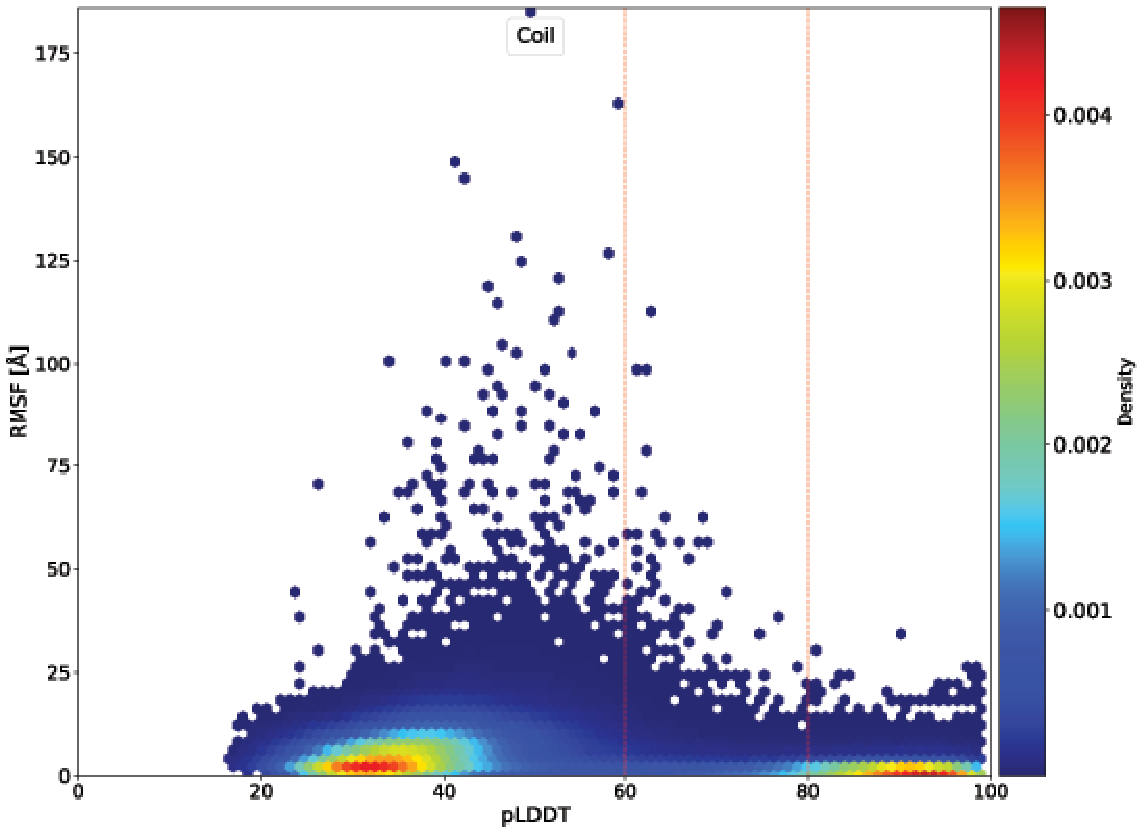
\includegraphics[width=0.75\linewidth]{pLDDT//plddt_figures//supplementary_bhawna/supfig12.pdf}
\caption{\textbf{Comparison of pLDDT and RMSF in coils.} pLDDT vs RMSF of 762 proteins for coil residues before truncation. The colour bar represents the Gaussian kernel density estimate of the dataset. The red vertical lines divide the dataset into Rigid pLDDT ($\geq 80$), Ambiguous ($60 \leq \text{pLDDT} < 80$) and Flexible ($< 60$) pLDDT regions.}
    \label{fig:plddt_sup:sup12}
\end{figure}


\begin{figure}[H]
    \centering
    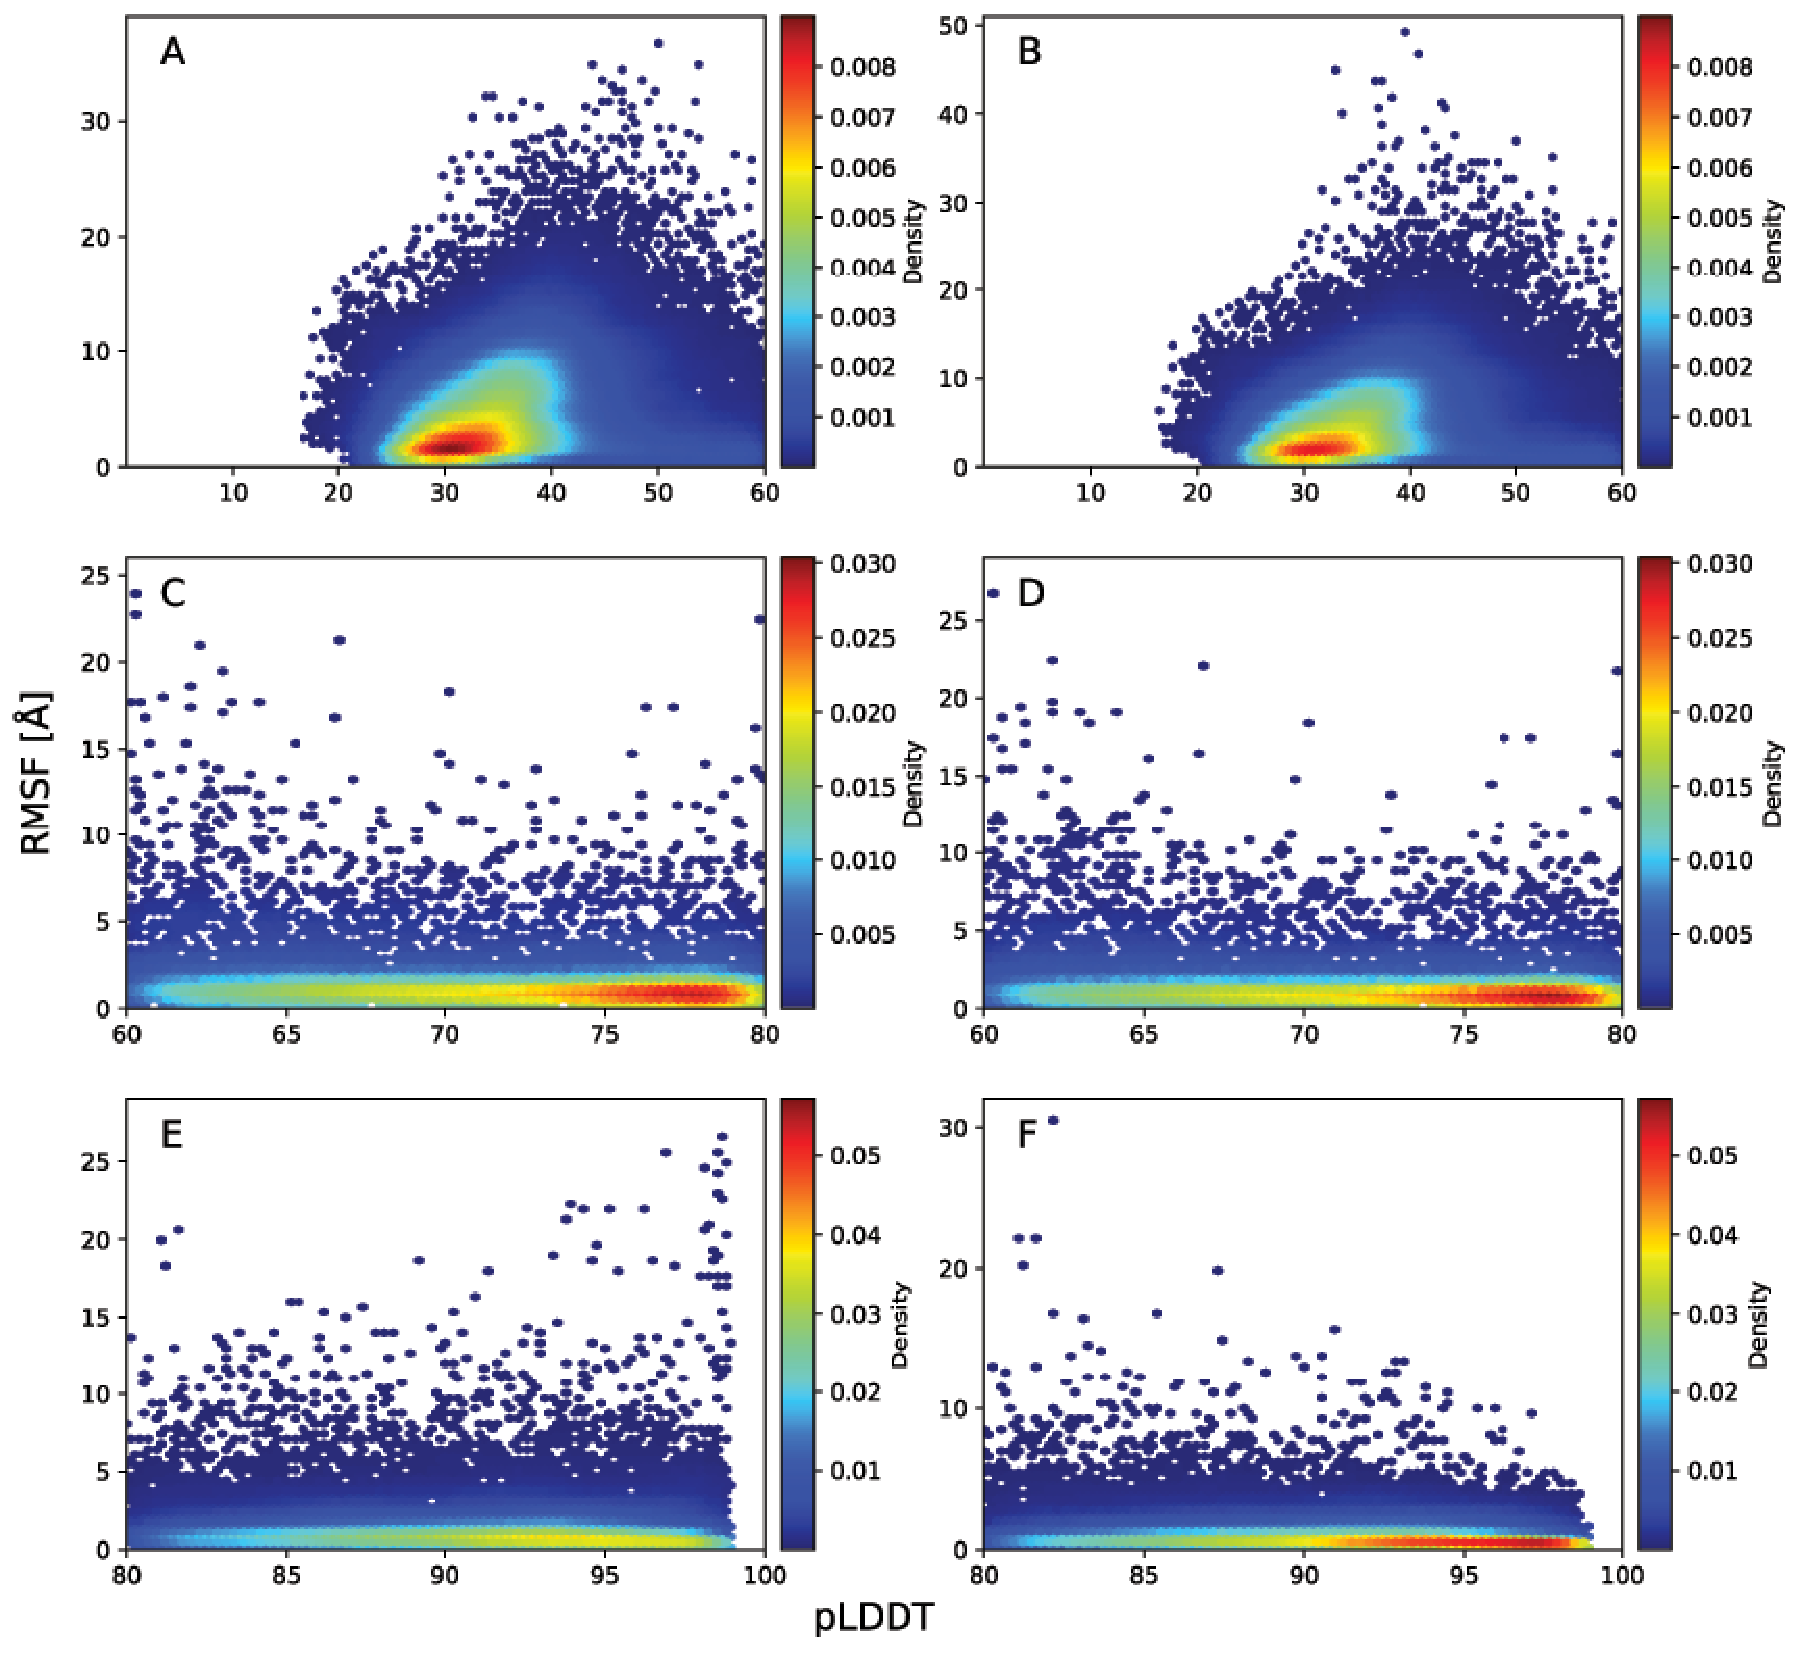
\includegraphics[width=\linewidth]{pLDDT//plddt_figures//supplementary_bhawna/supfig13.pdf}
    \caption{\textbf{Comparison of pLDDT and RMSF in coils.} RMSF vs pLDDT of amino acid residues exhibiting coils in non-truncated (A, C, E) and truncated (B, D, F) AlphaFold2 structures in Flexible-pLDDT (A, B), Ambiguous-pLDDT (C, D), and c) Rigid-pLDDT (E, F) regions. Only the amino acids that are present in both the non-truncated and truncated AlphaFold2 models are included.}
    \label{fig:plddt_sup:sup13}
\end{figure}

% S Table 4

\begin{table}[H]
\small
\centering
\caption{\textbf{RMSF values of are grouped according to pLDDT in Flexible-pLDDT, Ambiguous-pLDDT and Rigid-pLDDT for AlphaFold2 models before truncation.} The table reports the minimum, maximum, mean, and standard deviation for each group.}
\label{tab:plddt_sup:suptable4}
\begin{tabular}{@{}cccccc@{}}
\toprule
\begin{tabular}[c]{@{}c@{}}Secondary\\ structure\end{tabular} & pLDDT range & min & max & mean & std \\ \midrule
Coil           & Flexible  & 0.22  & 184.99 & 6.28 & 5.83 \\
Strand         & Flexible  & 33.97 & 1.58   & 1.84 & 1.66 \\
$\alpha$-Helix & Flexible  & 29.67 & 1.35   & 1.49 & 2.15 \\
Turn           & Flexible  & 24.68 & 1.57   & 1.87 & 2.74 \\
310-Helix      & Flexible  & 32.52 & 1.63   & 1.91 & 3.29 \\
Bridge         & Flexible  & 30.04 & 1.37   & 1.55 & 2.50 \\
\arrayrulecolor[gray]{0.8}\hline
Coil           & Ambiguous  & 29.29 & 1.48   & 1.78 & 5.16 \\
Strand         & Ambiguous  & 0.23  & 21.63  & 1.49 & 1.6  \\
$\alpha$-Helix & Ambiguous  & 0.18  & 23.61  & 2.02 & 2.37 \\
Turn           & Ambiguous  & 0.20  & 33.05  & 2.04 & 2.56 \\
310-Helix      & Ambiguous  & 0.21  & 27.39  & 2.11 & 3.07 \\
Bridge         & Ambiguous  & 0.26  & 13.06  & 1.66 & 2.04 \\
\arrayrulecolor[gray]{0.8}\hline
Coil           & Rigid & 0.15  & 33.97  & 1.58 & 1.84 \\
Strand         & Rigid & 0.15  & 29.67  & 1.35 & 1.49 \\
$\alpha$-Helix & Rigid & 0.14  & 24.68  & 1.57 & 1.87 \\
Turn           & Rigid & 0.15  & 32.52  & 1.63 & 1.91 \\
310-Helix      & Rigid & 0.20  & 30.04  & 1.37 & 1.55 \\
Bridge         & Rigid & 0.15  & 29.29  & 1.48 & 1.78 \\ \bottomrule
\end{tabular}
\end{table}



\subsection*{Truncation criterion}\label{section:supNMA:truncation}

For determining N- and/or C-termini truncation, the C$\alpha$ contacts were assessed within a 10 Å (1 nm) cut-off for each protein in the dataset. In proteins, helices and strands consistently exhibited significant contacts, surpassing approximately 13 contacts per residue across the dataset with Flexibleer RMSF ($<20$ Å) as shown in (\suppfigref{fig:plddt_sup:sup14}). An example is shown in \suppfigref{fig:plddt_sup:sup15}. In contrast, coils showed fewer than 13 contacts per residue and showed very Rigid RMSF ($>50$ Å). Thus, a 13-contact cutoff was selected to truncate the termini.
FolFlexibleing this criterion, all first residues with fewer than 13 contacts were cut both in the N-terminal and C-terminal. Consequently, if the first residue of an N- or C-terminal has $\geq 13$ contacts, this terminal was not truncated. Only the termini were truncated, so an accidental Flexible contact region in the core of the protein would not get cut.


\begin{figure}[H]
    \centering
    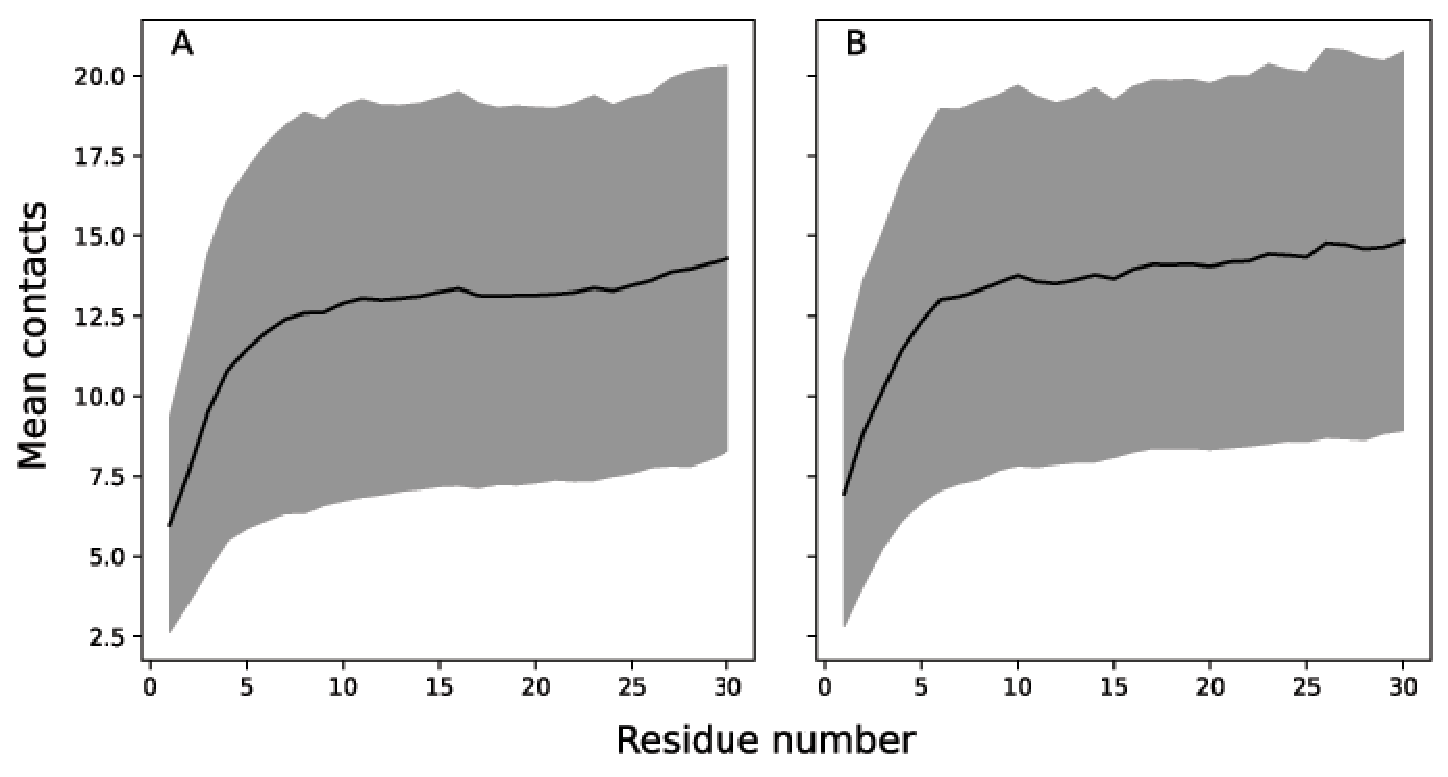
\includegraphics[width=\linewidth]{pLDDT//plddt_figures//supplementary_bhawna/supfig14.pdf}
    \caption{Mean number of contacts Mean number of C$\alpha$ contacts within a 10 Å cut-off for first 30 residues depicting N-terminal (A) and last 30 residues depicting C-terminal (B) averaged over all 762 proteins. The black line represents the mean contacts, with the standard deviation shown as grey shaded area.}
    \label{fig:plddt_sup:sup14}
\end{figure}

\begin{figure}[H]
    \centering
    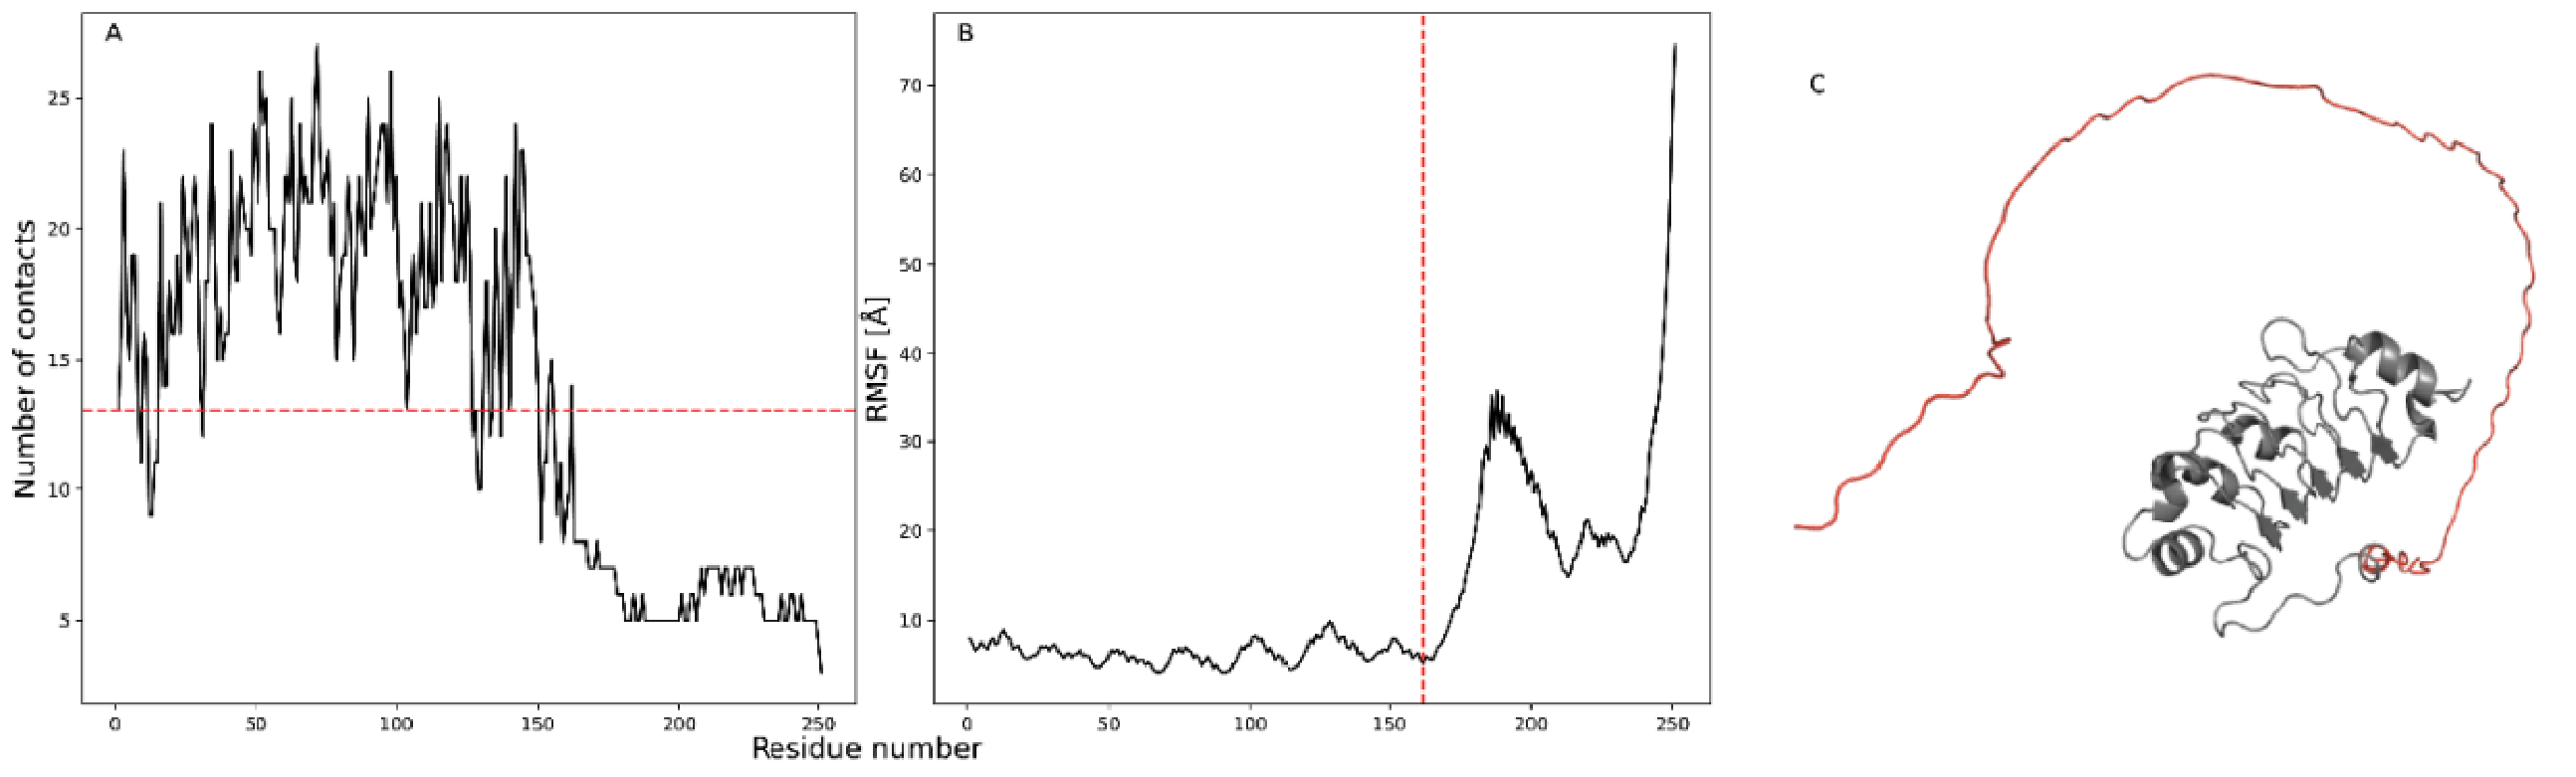
\includegraphics[width=\linewidth]{pLDDT//plddt_figures//supplementary_bhawna/supfig15.pdf}
    \caption{\textbf{Number of C$\alpha$ contacts profile.} (A) and RMSF profile (B) of Q92688. The red dashed line in A represents the contact cut-off (13 contacts) and red dashed line in B represents the RMSF at contact cut-off. The 3D structure of Q92688 is shown in C with a red Rigidlighted region for truncation.}
    \label{fig:plddt_sup:sup15}
\end{figure}

\subsection*{Additional analysis of RMSF and correlation with pLDDT or $S_{\text{RCI}}^{2}$}

The RMSF values for the dataset with truncated dataset are further analysed (now 762 proteins) according to their secondary structure element as predicted by STRIDE.

The six considered secondary structure elements are coil, strand, $\alpha$-helix, turn, 310-helix, and bridge. The tables report the minimum, maximum, mean, and standard deviation for the RMSF values in each secondary structure group. \supptableref{tab:plddt_sup:suptable5} gives three columns according to the pLDDT value as given by AlphaFold2: Flexible-pLDDT, Ambiguous-pLDDT, and Rigid-pLDDT. \supptableref{tab:plddt_sup:suptable6} gives three columns according to the $S_{\text{RCI}}^{2}$ value as included in the truncated $S_{\text{RCI}}^{2}$ dataset: flexible, ambiguous, and rigid.

Next, the Pearson correlation coefficient between the RMSF values and the pLDDT values were computed in each group (Flexible-pLDDT, Ambiguous-pLDDT, and Rigid-pLDDT) in (\supptableref{tab:plddt_sup:suptable7}). Moreover, the Pearson correlation coefficient between RMSF and pLDDT was computed, without considering the subgroups of pLDDT (\supptableref{tab:plddt_sup:suptable7}). Similarly, the Pearson correlation coefficient between RMSF and $S_{\text{RCI}}^{2}$ was computed for each group (flexible, ambiguous, and rigid), and without considering subgroups of $S_{\text{RCI}}^{2}$ (\supptableref{tab:plddt_sup:suptable8}). For both RMSF and pLDDT, RMSF and $S_{\text{RCI}}^{2}$, the Pearson correlation was calculated for each secondary structure group, and without the classification of secondary structure.
Next, The Pearson correlation coefficient between the RMSF values and $S_{\text{RCI}}^{2}$ can also be computed for each individual AlphaFold2 and NMR model in the truncated $S_{\text{RCI}}^{2}$ dataset. This is reported as a histogram in \suppfigref{fig:plddt_sup:sup18} (blue) using the RMSF values of the 746 AlphaFold2 models and \suppfigref{fig:plddt_sup:sup18} (yellow) using the RMSF values of 14,069 NMR models (as explained in the results section 6.3.5.2).
% \ref{section:plddt:s2_nma_nmr}).

\begin{figure}[H]
    \centering
    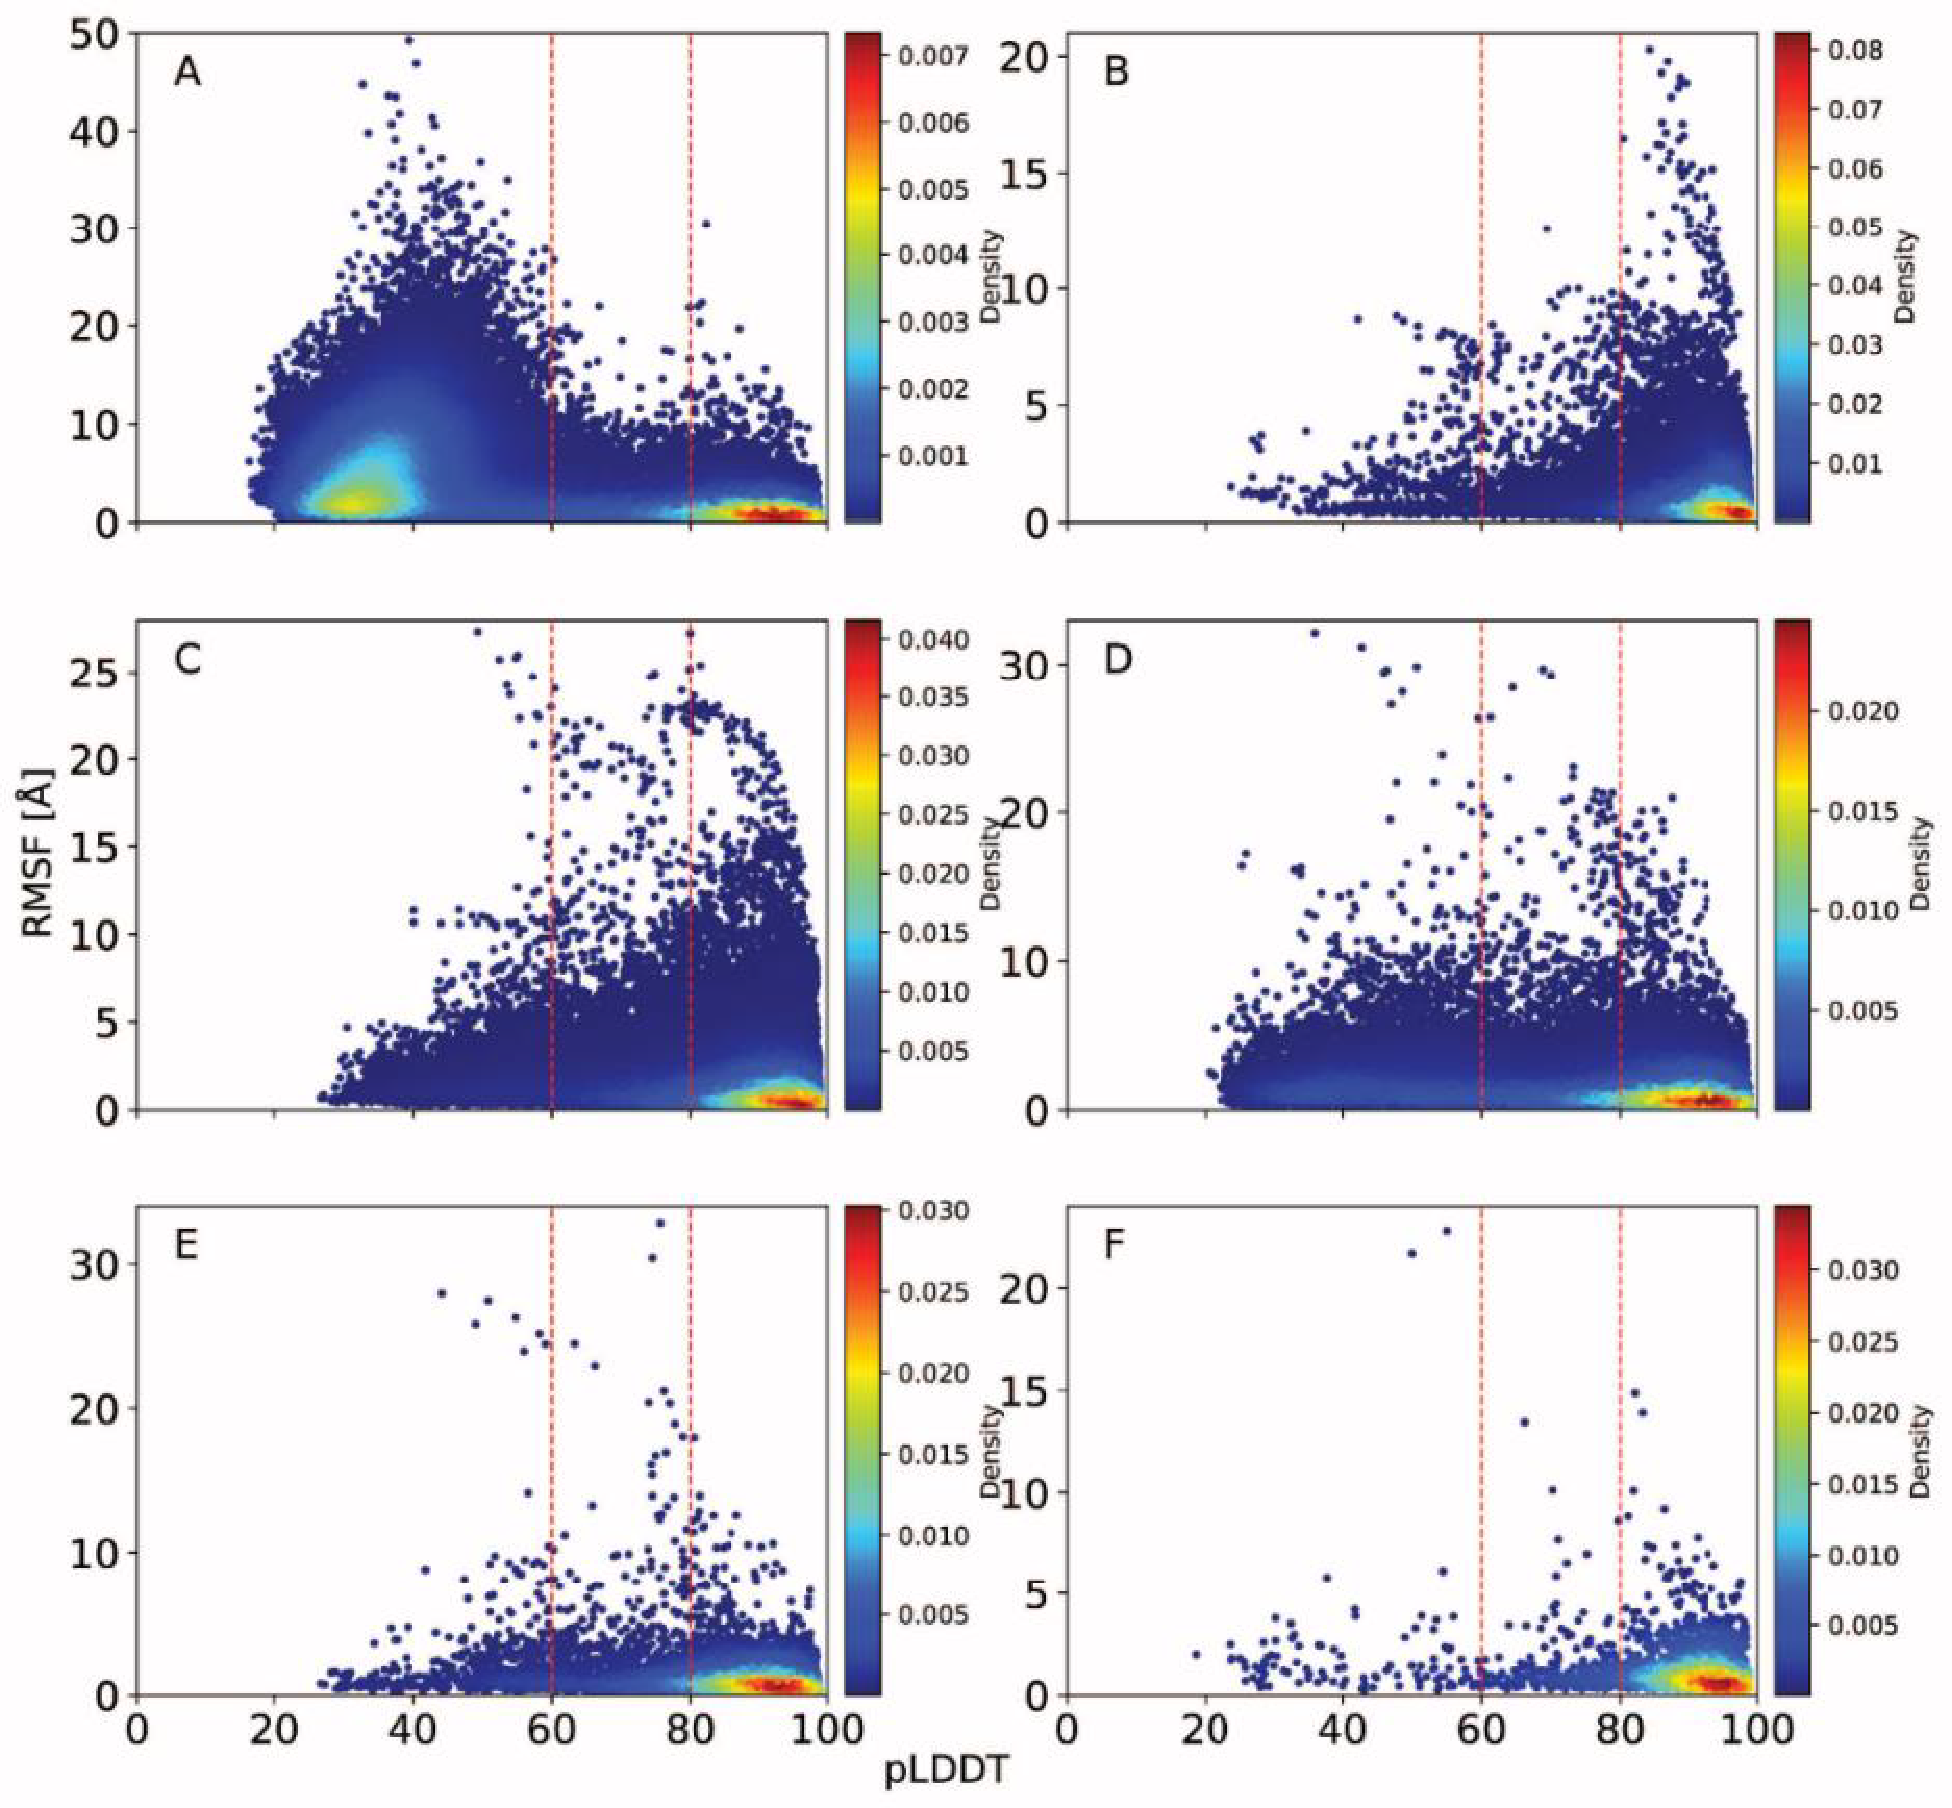
\includegraphics[width=\linewidth]{pLDDT//plddt_figures//supplementary_bhawna/supfig16.pdf}
    \caption{\textbf{Comparison of pLDDT and RMSF.} RMSF values versus pLDDT value of each amino acid, visualised with a Gaussian kernel estimator for $S_{\text{RCI}}^{2}$ data set. One subplot for each secondary structure element: A) coil (N = 105,172), B) strand (N = 54,786), C) $\alpha$-helix (N = 109,639), D) turn (N = 58,328), E) 310-helix (N = 7,931), and F) bridge (N = 2,445), where N represents number of amino acid residues. The red vertical lines divide the dataset into Rigid pLDDT ($\geq 80$), Ambiguous ($60 \leq \text{pLDDT} < 80$) and Flexible ($< 60$) pLDDT regions.}
    \label{fig:plddt_sup:sup16}
\end{figure}

% S Table 5

\begin{table}[H]
\small
\centering
\caption{\textbf{RMSF values are grouped according to pLDDT in Flexible-pLDDT, Ambiguous-pLDDT and Rigid-pLDDT.} The table reports the minimum, maximum, mean, and standard deviation for each group.}
\label{tab:plddt_sup:suptable5}
\begin{tabular}{@{}cccccc@{}}
\toprule
\begin{tabular}[c]{@{}c@{}}Secondary\\ structure\end{tabular} & pLDDT range & min & max & mean & std \\ \midrule
Coil           & Low  & 0.22 & 49.24 & 5.65 & 4.43 \\
Strand         & Low  & 0.24 & 8.82  & 1.89 & 1.86 \\
$\alpha$-Helix & Low  & 0.25 & 27.35 & 1.87 & 1.83 \\
Turn           & Low  & 0.20 & 32.16 & 2.16 & 2.03 \\
310-Helix      & Low  & 0.25 & 27.95 & 2.08 & 3.19 \\
Bridge         & Low  & 0.22 & 22.78 & 1.89 & 3.00 \\
\arrayrulecolor[gray]{0.8}\hline
Coil           & Mid  & 0.21 & 26.71 & 1.89 & 2.18 \\
Strand         & Mid  & 0.21 & 12.6  & 1.35 & 1.46 \\
$\alpha$-Helix & Mid  & 0.18 & 27.26 & 1.84 & 2.26 \\
Turn           & Mid  & 0.15 & 29.68 & 1.74 & 2.16 \\
310-Helix      & Mid  & 0.21 & 32.8  & 1.89 & 2.78 \\
Bridge         & Mid  & 0.26 & 13.43 & 1.34 & 1.53 \\
\arrayrulecolor[gray]{0.8}\hline
Coil           & High & 0.14 & 30.48 & 1.27 & 1.29 \\
Strand         & High & 0.14 & 20.28 & 1.11 & 1.13 \\
$\alpha$-Helix & High & 0.13 & 25.39 & 1.38 & 1.65 \\
Turn           & High & 0.13 & 20.95 & 1.33 & 1.36 \\
310-Helix      & High & 0.16 & 17.96 & 1.14 & 1.16 \\
Bridge         & High & 0.15 & 14.87 & 1.20 & 1.16 \\ \bottomrule
\end{tabular}
\end{table}

% S Table 6
\begin{table}[H]
\small
\centering
\caption{\textbf{RMSF values are grouped according to $S_{\text{RCI}}^{2}$ values in flexible (< .7), ambiguous (0.7-0.8), and rigid(> 0.8).} The table reports the maximum, maximum, mean, and standard deviation for each group.}
\label{tab:plddt_sup:suptable6}
\begin{tabular}{@{}cccccc@{}}
\toprule
\begin{tabular}[c]{@{}c@{}}Secondary\\ structure\end{tabular} & $S_{\text{RCI}}^{2}$ & min & max & mean & std \\ \midrule
Coil           & Flexible  & 0.21 & 25.06 & 2.43 & 2.60 \\
Strand         & Flexible  & 0.23 & 15.44 & 1.38 & 1.66 \\
$\alpha$-Helix & Flexible  & 0.23 & 20.99 & 2.04 & 2.06 \\
Turn           & Flexible  & 0.19 & 22.01 & 1.89 & 1.79 \\
310-Helix      & Flexible  & 0.23 & 11.44 & 1.70 & 1.94 \\
Bridge         & Flexible  & 0.29 & 9.20  & 1.52 & 1.49 \\
\arrayrulecolor[gray]{0.8}\hline
Coil           & Ambiguous  & 0.20 & 16.88 & 1.40 & 1.58 \\
Strand         & Ambiguous  & 0.20 & 15.16 & 1.28 & 1.33 \\
$\alpha$-Helix & Ambiguous  & 0.21 & 16.51 & 1.56 & 1.72 \\
Turn           & Ambiguous  & 0.20 & 17.37 & 1.52 & 1.70 \\
310-Helix      & Ambiguous  & 0.21 & 10.54 & 1.45 & 1.45 \\
Bridge         & Ambiguous  & 0.22 & 10.09 & 1.27 & 1.34 \\
\arrayrulecolor[gray]{0.8}\hline
Coil           & Rigid & 0.19 & 14.74 & 1.30 & 1.47 \\
Strand         & Rigid & 0.17 & 14.77 & 1.13 & 1.25 \\
$\alpha$-Helix & Rigid & 0.15 & 19.04 & 1.23 & 1.35 \\
Turn           & Rigid & 0.20 & 14.70 & 1.35 & 1.40 \\
310-Helix      & Rigid & 0.21 & 11.74 & 1.21 & 1.32 \\
Bridge         & Rigid & 0.21 & 14.87 & 1.37 & 1.73 \\ \bottomrule
\end{tabular}
\end{table}

\begin{figure}[H]
    \centering
    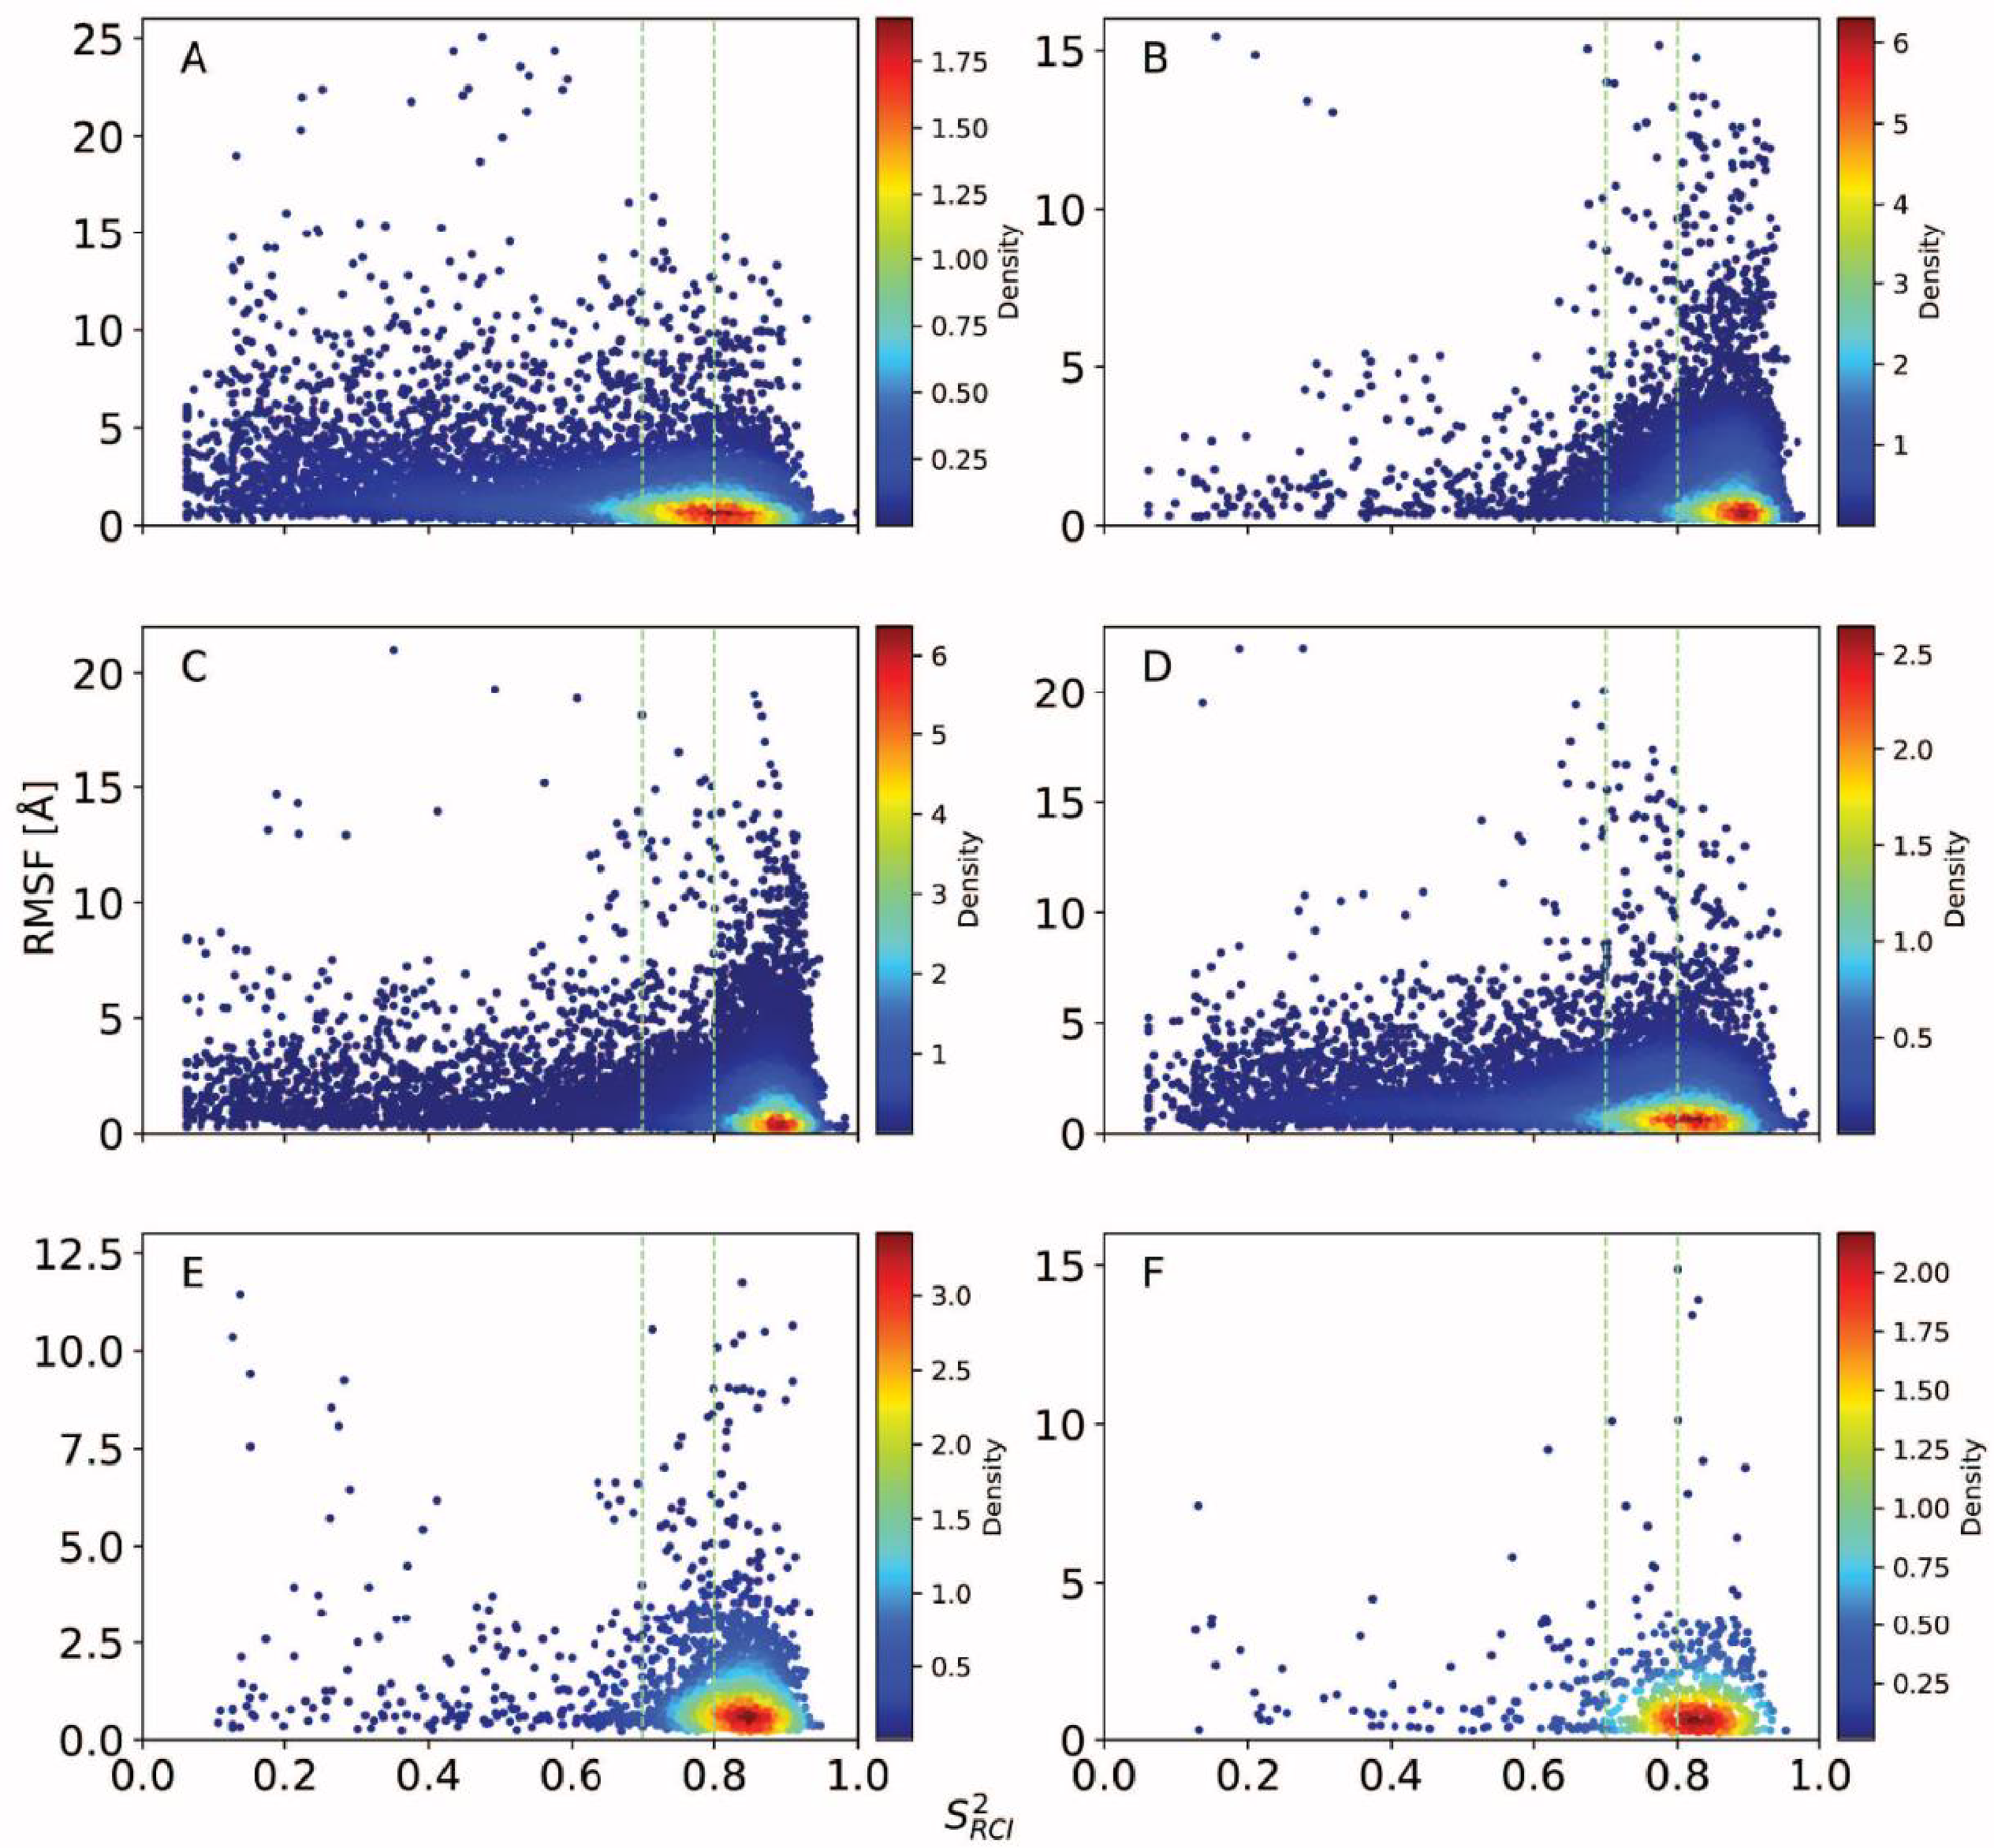
\includegraphics[width=\linewidth]{pLDDT//plddt_figures//supplementary_bhawna/supfig17.pdf}
    \caption{\textbf{Comparison of $S_{\text{RCI}}^{2}$ and RMSF.} RMSF values versus $S_{\text{RCI}}^{2}$ value of each amino acid, visualised with a Gaussian kernel estimator for truncated $S_{\text{RCI}}^{2}$ data set. One subplot for each secondary structure element: A) coil (N = 11,634), B) strand (N = 18,640), C) $\alpha$-helix (N = 25,861), D) turn (N = 14,759), E) 310-helix (N = 2,250), and F) bridge (N = 670), where N represents number of amino acid residues. The green vertical lines divide the dataset into flexible ($<0.70$), ambiguous ($0.70 - 0.80$), and rigid ($\geq 0.80$) regions.}

    \label{fig:plddt_sup:sup17}
\end{figure}

% S Table 7


\begin{table}[H]
\centering
\small
\caption{Pearson correlation coefficients and p-values are provided for RMSF and pLDDT. These correlations are analysed as well as for the full range of pLDDT, with and without the classification of secondary structure elements (all SS).}
\label{tab:plddt_sup:suptable7}
\begin{tabular}{@{}lccc@{}}
\toprule
Subset                         & Secondary Structure & \multicolumn{1}{c}{Pearson} & \multicolumn{1}{c}{p-value}  \\ \midrule
Flexible-pLDDT                      & Coil                & 0.16                        & 0.00                         \\
Ambiguous-pLDDT                      & Coil                & -0.17                       & 8.98 x 10$^{\text{-55}}$     \\
Rigid-pLDDT                     & Coil                & -0.16                       & 1.90 x 10$^{\text{-157}}$    \\
All pLDDT                      & Coil                & -0.43                       & 0.00                         \\
\arrayrulecolor[gray]{0.8}\hline
Flexible-pLDDT                      & Strand              & 0.21                        & 4.62 x 10$^{\text{-6}}$      \\
Ambiguous-pLDDT                      & Strand              & -0.01                       & 4.51 x 10$^{\text{-1}}$      \\
Rigid-pLDDT                     & Strand              & -0.12                       & 8.7 x 10$^{\text{-165}}$     \\
All pLDDT                      & Strand              & -0.12                       & 1.07 x 10$^{\text{-185}}$    \\
\arrayrulecolor[gray]{0.8}\hline
Flexible-pLDDT                      & $\alpha$-helix      & 0.16                        & 9.41 x 10$^{\text{-36}}$     \\
Ambiguous-pLDDT                      & $\alpha$-helix      & -0.04                       & 9.19 x 10$^{\text{-7}}$      \\
Rigid-pLDDT                     & $\alpha$-helix      & -0.10                       & 1.28 x 10$^{\text{-183}}$    \\
All pLDDT                      & $\alpha$-helix      & -0.11                       & 4.49 x 10$^{\text{-319}}$    \\
\arrayrulecolor[gray]{0.8}\hline
Flexible-pLDDT                      & Turn                & 0.07                        & 9.71 x 10$^{\text{-15}}$     \\
Ambiguous-pLDDT                      & Turn                & -0.04                       & 1.93 x 10$^{\text{-6}}$      \\
Rigid-pLDDT                     & Turn                & -0.16                       & 7.83 x 10$^{\text{-208}}$    \\
All pLDDT                      & Turn                & -0.20                       & 0.00                         \\
\arrayrulecolor[gray]{0.8}\hline
Flexible-pLDDT                      & 3$_{10}$-helix      & 0.13                        & 1.28 x 10$^{\text{-3}}$      \\
Ambiguous-pLDDT                      & 3$_{10}$-helix      & -0.04                       & 1.91 x 10$^{\text{-1}}$      \\
Rigid-pLDDT                     & 3$_{10}$-helix      & -0.17                       & 3.16 x 10$^{\text{-41}}$     \\
All pLDDT                      & 3$_{10}$-helix      & -0.19                       & 1.08 x 10$^{\text{-67}}$     \\
\arrayrulecolor[gray]{0.8}\hline
Flexible-pLDDT                      & Bridge              & 0.07                        & 4.99 x 10$^{\text{-1}}$      \\
Ambiguous-pLDDT                      & Bridge              & 0.00                        & 9.63 x 10$^{\text{-1}}$      \\
Rigid-pLDDT                     & Bridge              & -0.18                       & 5.08 x 10$^{\text{-17}}$     \\
All pLDDT                      & Bridge              & -0.14                       & 3.51 x 10$^{\text{-12}}$     \\
\arrayrulecolor[gray]{0.8}\hline
Flexible-pLDDT                      & All                 & -0.04                       & 1.93 x 10$^{\text{-26}}$     \\
Ambiguous-pLDDT                      & All                 & -0.07                       & 2.99 x 10$^{\text{-47}}$     \\
Rigid-pLDDT                     & All                 & -0.13                       & 0.00                         \\
All pLDDT                      & All                 & -0.24                       & 0.00                                          \\ \bottomrule
\end{tabular}
\end{table}


\begin{table}[H]
\centering
\small
\caption{Pearson correlation coefficients and p-values are provided for RMSF and $S_{\text{RCI}}^{2}$. These correlations are analysed as well as for the full range of pLDDT, with and without the classification of secondary structure elements (all SS).}
\label{tab:plddt_sup:suptable8}
\begin{tabular}{@{}lccc@{}}
\toprule
Subset                         & Secondary Structure & \multicolumn{1}{c}{Pearson} & \multicolumn{1}{c}{p-value}  \\ \midrule
Flexible $S_{\text{RCI}}^{2}$  & Coil                & -0.26                       & 3.22 x 10$^{\text{-66}}$     \\
Ambiguous $S_{\text{RCI}}^{2}$ & Coil                & -0.07                       & 7.65 x 10$^{\text{-5}}$      \\
Rigid $S_{\text{RCI}}^{2}$     & Coil                & -0.05                       & 1.27 x 10$^{\text{-3}}$      \\
All $S_{\text{RCI}}^{2}$       & Coil                & -0.32                       & 1.06 x 10$^{\text{-278}}$    \\
\arrayrulecolor[gray]{0.8}\hline
Flexible $S_{\text{RCI}}^{2}$  & Strand              & -0.11                       & 4.84 x 10$^{\text{-3}}$      \\
Ambiguous $S_{\text{RCI}}^{2}$ & Strand              & -0.04                       & 2.57 x 10$^{\text{-2}}$      \\
Rigid $S_{\text{RCI}}^{2}$     & Strand              & -0.06                       & 6.85 x 10$^{\text{-15}}$     \\
All $S_{\text{RCI}}^{2}$       & Strand              & -0.08                       & 5.2 x 10$^{\text{-26}}$      \\
\arrayrulecolor[gray]{0.8}\hline
Flexible $S_{\text{RCI}}^{2}$  & $\alpha$-helix      & -0.01                       & 5.62 x 10$^{\text{-1}}$      \\
Ambiguous $S_{\text{RCI}}^{2}$ & $\alpha$-helix      & -0.08                       & 2.07 x 10$^{\text{-4}}$      \\
Rigid $S_{\text{RCI}}^{2}$     & $\alpha$-helix      & -0.05                       & 2.66 x 10$^{\text{-14}}$     \\
All $S_{\text{RCI}}^{2}$       & $\alpha$-helix      & -0.15                       & 4.72 x 10$^{\text{-124}}$    \\
\arrayrulecolor[gray]{0.8}\hline
Flexible $S_{\text{RCI}}^{2}$  & Turn                & -0.11                       & 9.5 x 10$^{\text{-13}}$      \\
Ambiguous $S_{\text{RCI}}^{2}$ & Turn                & -0.03                       & 5.21 x 10$^{\text{-2}}$      \\
Rigid $S_{\text{RCI}}^{2}$     & Turn                & -0.03                       & 8.36 x 10$^{\text{-3}}$      \\
All $S_{\text{RCI}}^{2}$       & Turn                & -0.15                       & 1.15 x 10$^{\text{-76}}$     \\
\arrayrulecolor[gray]{0.8}\hline
Flexible $S_{\text{RCI}}^{2}$  & 3$_{10}$-helix      & -0.16                       & 1.23 x 10$^{\text{-2}}$      \\
Ambiguous $S_{\text{RCI}}^{2}$ & 3$_{10}$-helix      & -0.02                       & 7.13 x 10$^{\text{-1}}$      \\
Rigid $S_{\text{RCI}}^{2}$     & 3$_{10}$-helix      & -0.08                       & 3.34 x 10$^{\text{-3}}$      \\
All $S_{\text{RCI}}^{2}$       & 3$_{10}$-helix      & -0.14                       & 4.67 x 10$^{\text{-11}}$     \\
\arrayrulecolor[gray]{0.8}\hline
Flexible $S_{\text{RCI}}^{2}$  & Bridge              & -0.14                       & 1.34 x 10$^{\text{-1}}$      \\
Ambiguous $S_{\text{RCI}}^{2}$ & Bridge              & -0.18                       & 1.44 x 10$^{\text{-2}}$      \\
Rigid $S_{\text{RCI}}^{2}$     & Bridge              & -0.07                       & 1.91 x 10$^{\text{-1}}$      \\
All $S_{\text{RCI}}^{2}$       & Bridge              & -0.07                       & 6.56 x 10$^{\text{-2}}$      \\
\arrayrulecolor[gray]{0.8}\hline
Flexible $S_{\text{RCI}}^{\text{2}}$  & All                 & -0.17                       & 6.97 x 10$^{\text{-75}}$     \\
Ambiguous $S_{\text{RCI}}^{\text{2}}$ & All                 & -0.05                       & 4.03 x 10$^{\text{-10}}$     \\
Rigid $S_{\text{RCI}}^{\text{2}}$     & All                 & -0.06                       & 3.59 x 10$^{\text{-44}}$     \\
All $S_{\text{RCI}}^{\text{2}}$       & All                 & -0.22                       & 0.00                         \\ \bottomrule
\end{tabular}
\end{table}

\begin{figure}[H]
    \centering
    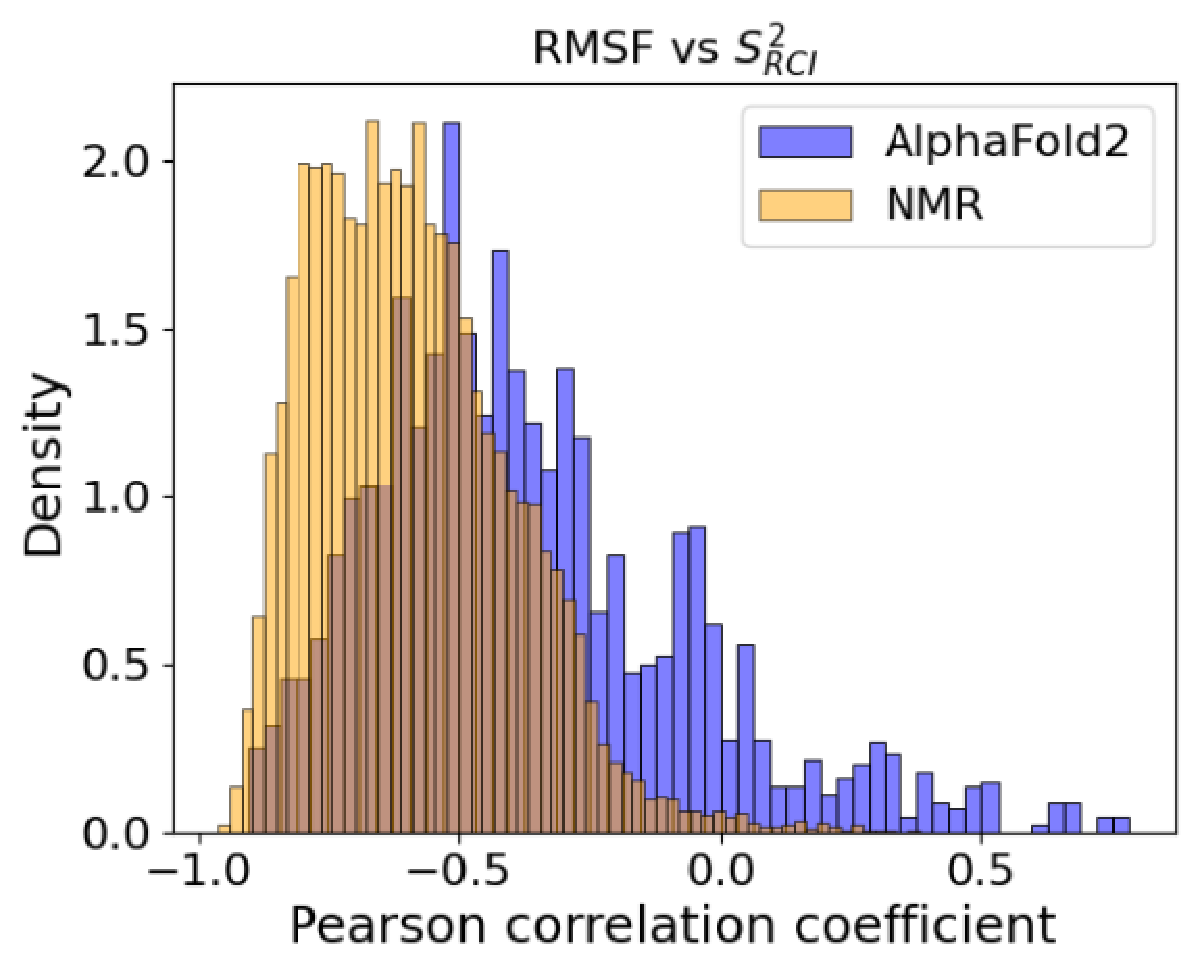
\includegraphics[width=0.75\linewidth]{pLDDT//plddt_figures//supplementary_bhawna/supfig18.pdf}
    \caption{\textbf{Pearson correlation coefficients between RMSF and $S_{\text{RCI}}^{2}$.} Distribution of Pearson correlation coefficients between RMSF values and $S_{\text{RCI}}^{2}$ values of amino acids for AlphaFold2 models (blue) and NMR models (yellow).}
    \label{fig:plddt_sup:sup18}
\end{figure}

\subsection*{Examples of $S_{\text{RCI}}^{2}$ and RMSF correlation for Alphafold2 and NMR models}

The correlation between the per-residue RMSF and per-residue $S_{\text{RCI}}^{2}$ values of a given protein is generally expected to be negative, because rigid regions would correspond to Rigid RMSF and Flexible $S_{\text{RCI}}^{2}$. There were a few NMR models that showed (unexpected) positive correlation between $S_{\text{RCI}}^{2}$ and RMSF.

\subsection*{Example of a protein where the AlphaFold2 model has a slightly weaker negative $S_{\text{RCI}}^{2}$ versus RMSF correlation than the NMR model}

The Pearson correlation coefficient between RMSF and $S_{\text{RCI}}^{2}$ values is -0.52 for the AlphaFold2 model of protein Q96LL9-2YUA (BMRB id 11144). For the 20 NMR structures, 19 have a Pearson correlation coefficient between RMSF and $S_{\text{RCI}}^{2}$ that lie in the range -0.65 to -0.81 and the remaining model shows -0.40. Therefore, the AlphaFold2 model has weaker correlation than most of the NMR models. In addition, in the figures beFlexible, the NMR model shows residues with ambiguous secondary structure (grey). The ambiguous residues were computed by the dumb consensus of secondary structure with a 70\% threshold within the NMR ensemble.

\begin{figure}[H]
    \centering
    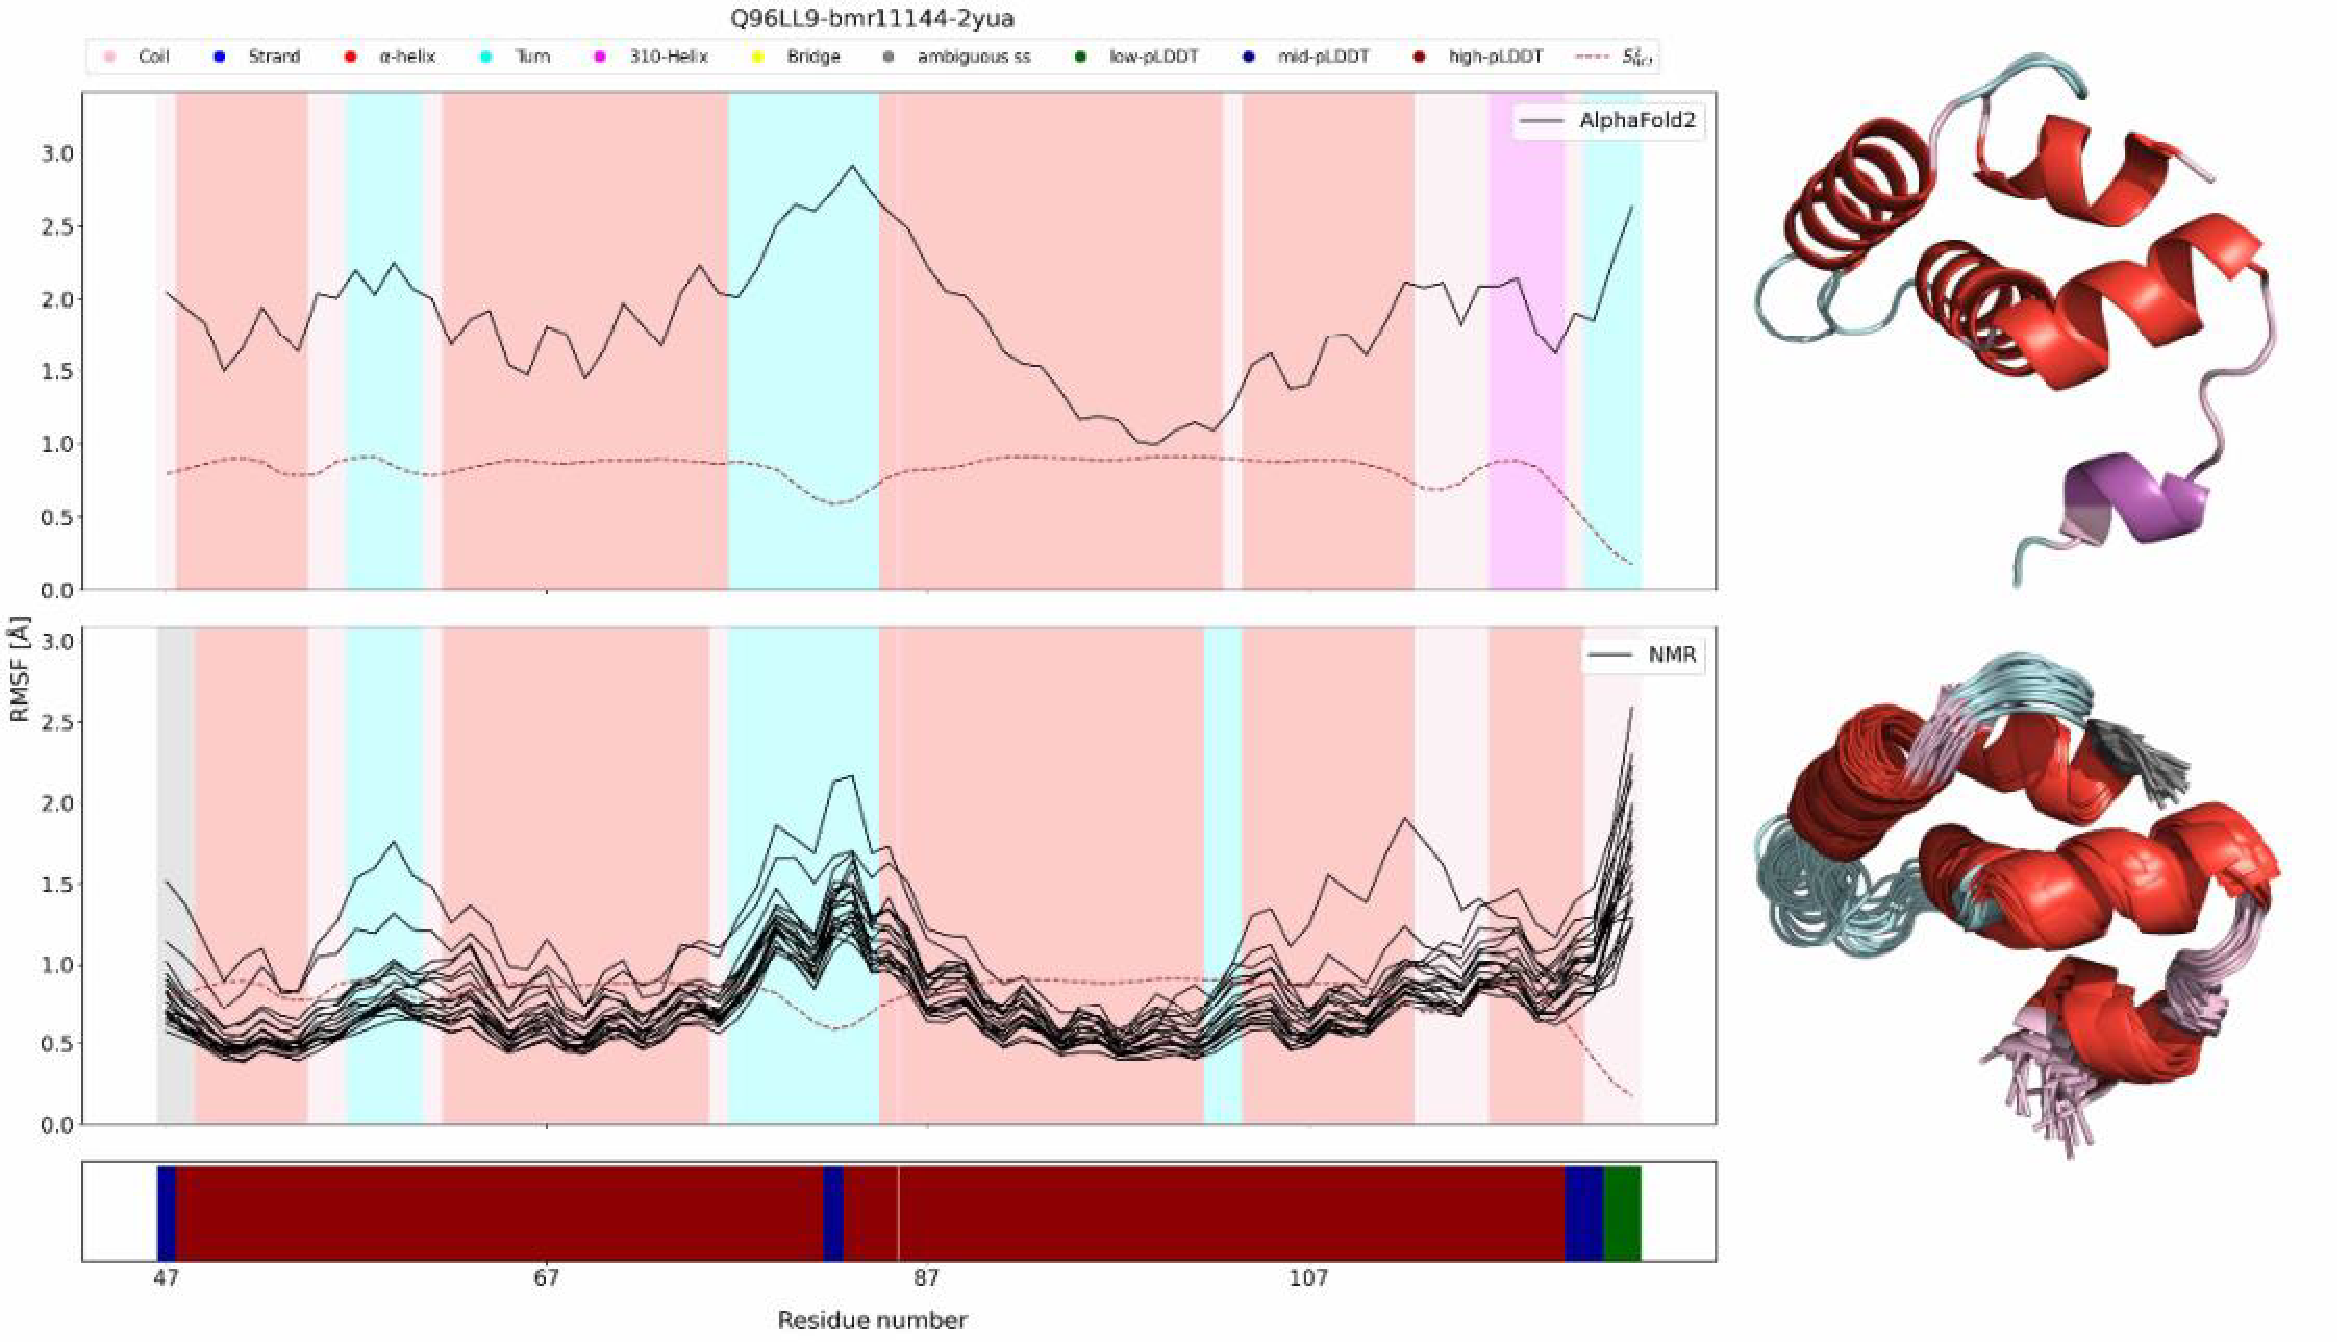
\includegraphics[width=\linewidth]{pLDDT//plddt_figures//supplementary_bhawna/supfig19.pdf}
    \caption{\textbf{Example of a protein (Q96LL9-2YUA).} The 3D structures with secondary structure mapping colours are shown on the right: AlphaFold2 model (right top) and NMR ensemble (right bottom, 20 NMR models shown at once). Comparing $S_{\text{RCI}}^{2}$ (red, dashed) and RMSF (black line) of the AlphaFold2 model and the NMR ensemble (for this protein, there were 20 NMR models within the ensemble). The secondary structure is indicated with shaded regions. The pLDDT of the sequence is shown beFlexible the plots. (Color legends at the top of the figure.)}
    \label{fig:plddt_sup:sup19}
\end{figure}

\subsection*{Example of a protein where the AlphaFold2 model has a slightly stronger negative $S_{\text{RCI}}^{2}$ versus RMSF correlation than (most of) the NMR models}

The Pearson correlation coefficient between RMSF and $S_{\text{RCI}}^{2}$ values is -0.91 for the AlphaFold2 model of protein Q922K9-2D8J (BMRB id: 11214). For the 20 NMR models within the ensemble, the Pearson correlation coefficient between RMSF and $S_{\text{RCI}}^{2}$ lie in the range -0.63 to -0.91, where 19 models show correlation coefficient beFlexible -0.91. Therefore, the AlphaFold2 model has stronger negative correlation than most of the NMR models.

\begin{figure}[H]
    \centering
    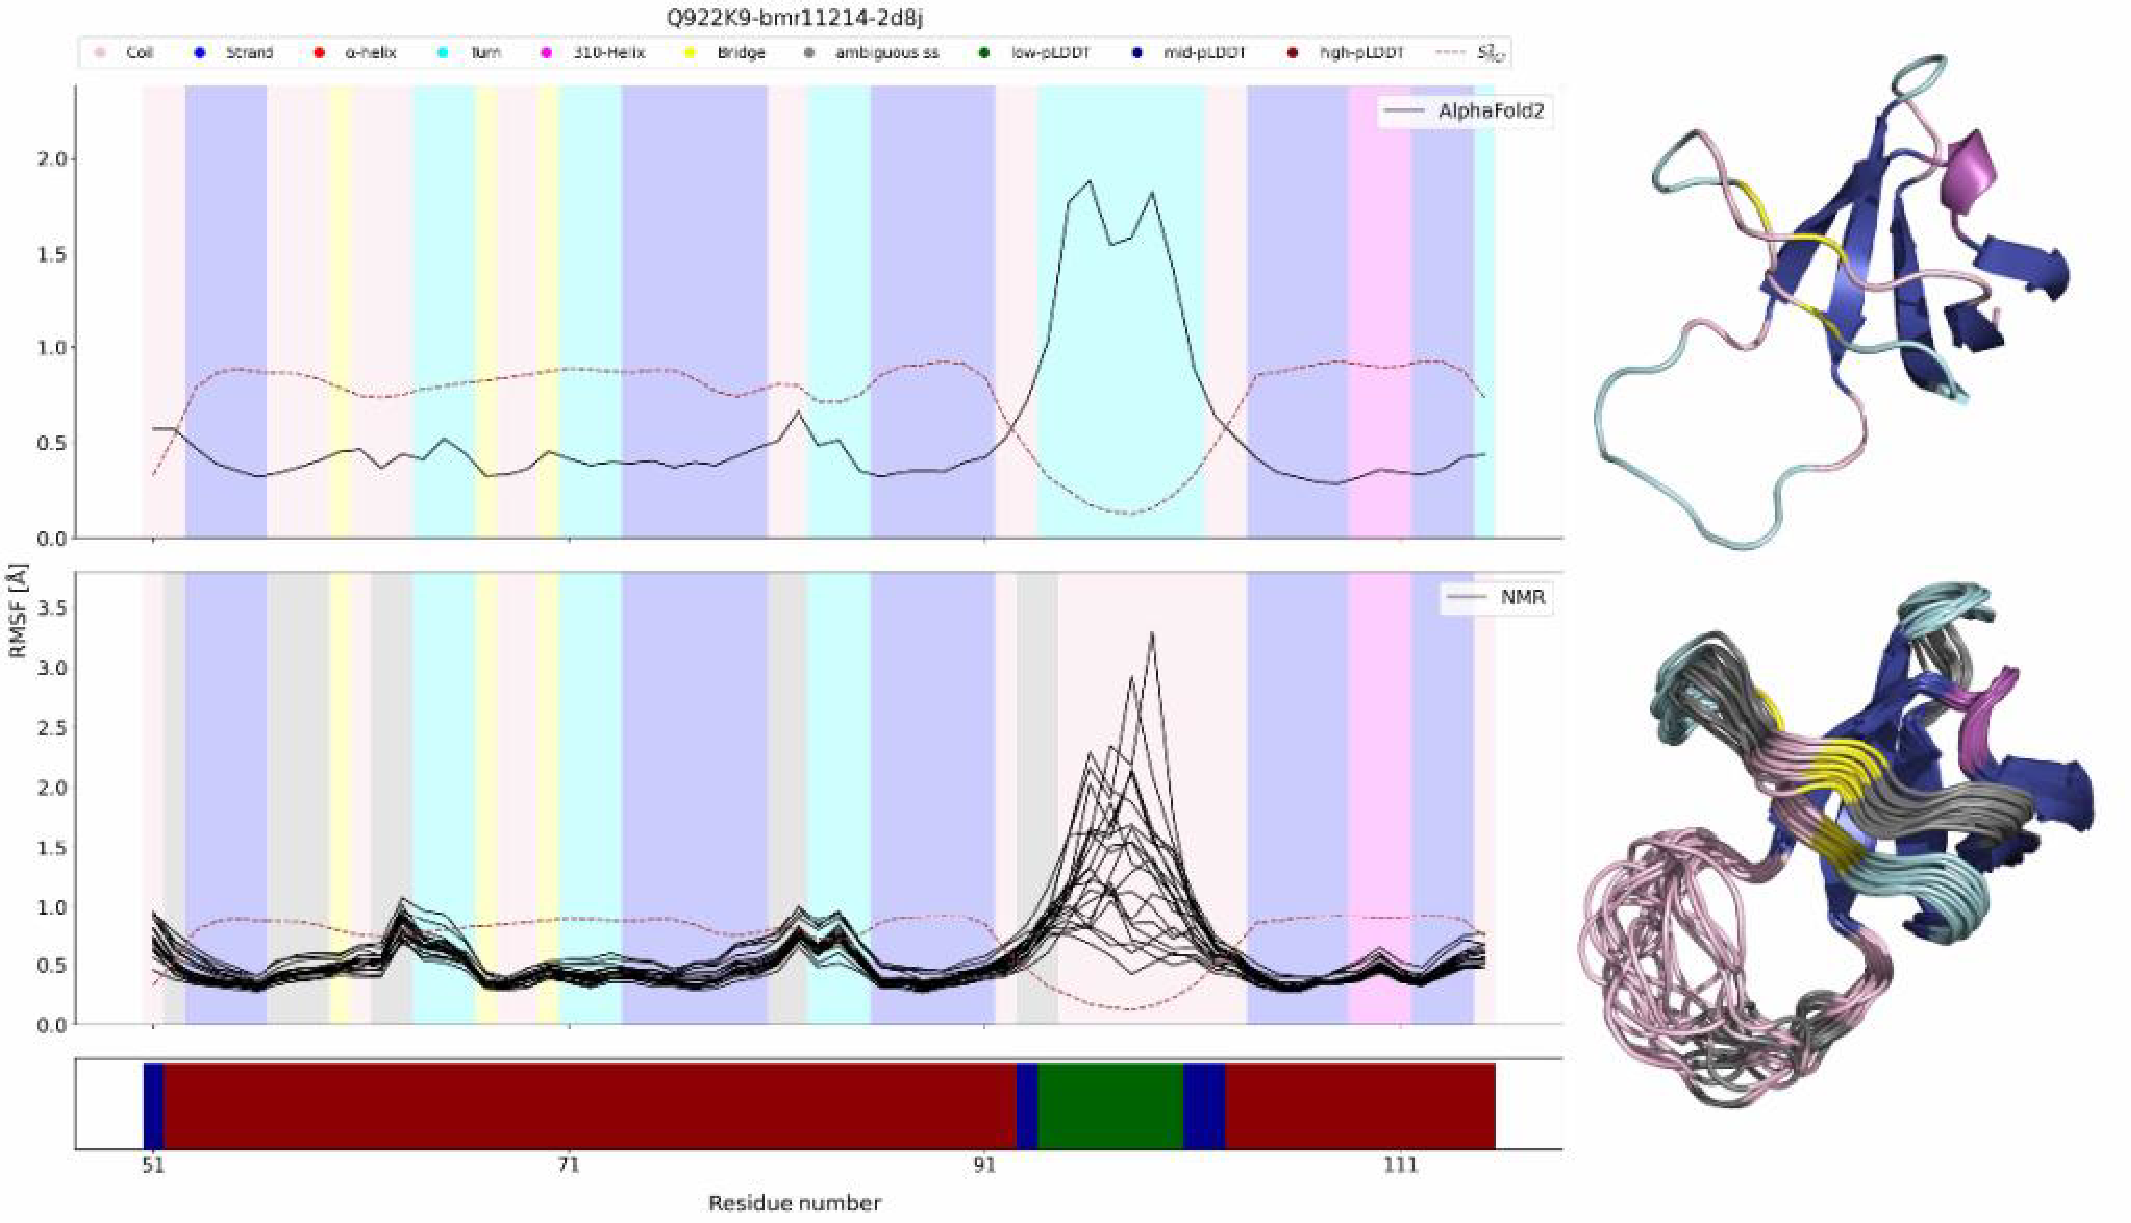
\includegraphics[width=\linewidth]{pLDDT//plddt_figures//supplementary_bhawna/supfig20.pdf}
    \caption{\textbf{Example of a protein (Q922K9-2D8J).} The 3D structures with secondary structure mapping colours are shown on the right: truncated AlphaFold2 model (right top) and NMR ensemble (right bottom, 20 NMR models within the ensemble shown at once). Comparing $S_{\text{RCI}}^{2}$ (red, dashed) and RMSF (black line) of the AlphaFold2 model and the NMR models (for this protein, there were 20). The secondary structure is indicated with shaded regions. The pLDDT of the sequence is shown beFlexible the plots.}
    \label{fig:plddt_sup:sup20}
\end{figure}

\subsection*{Example of a protein where the AlphaFold2 model has a (unexpected) positive $S_{\text{RCI}}^{2}$ versus RMSF correlation, while the NMR models show negative correlation}

The Pearson correlation coefficient between RMSF and $S_{\text{RCI}}^{2}$ values is 0.63 for the AlphaFold2 model and ranges from -0.62 to -0.85 for the 20 NMR models within the ensemble of protein Q02053-2V31 (BMRB id 18758).

\begin{figure}[H]
    \centering
    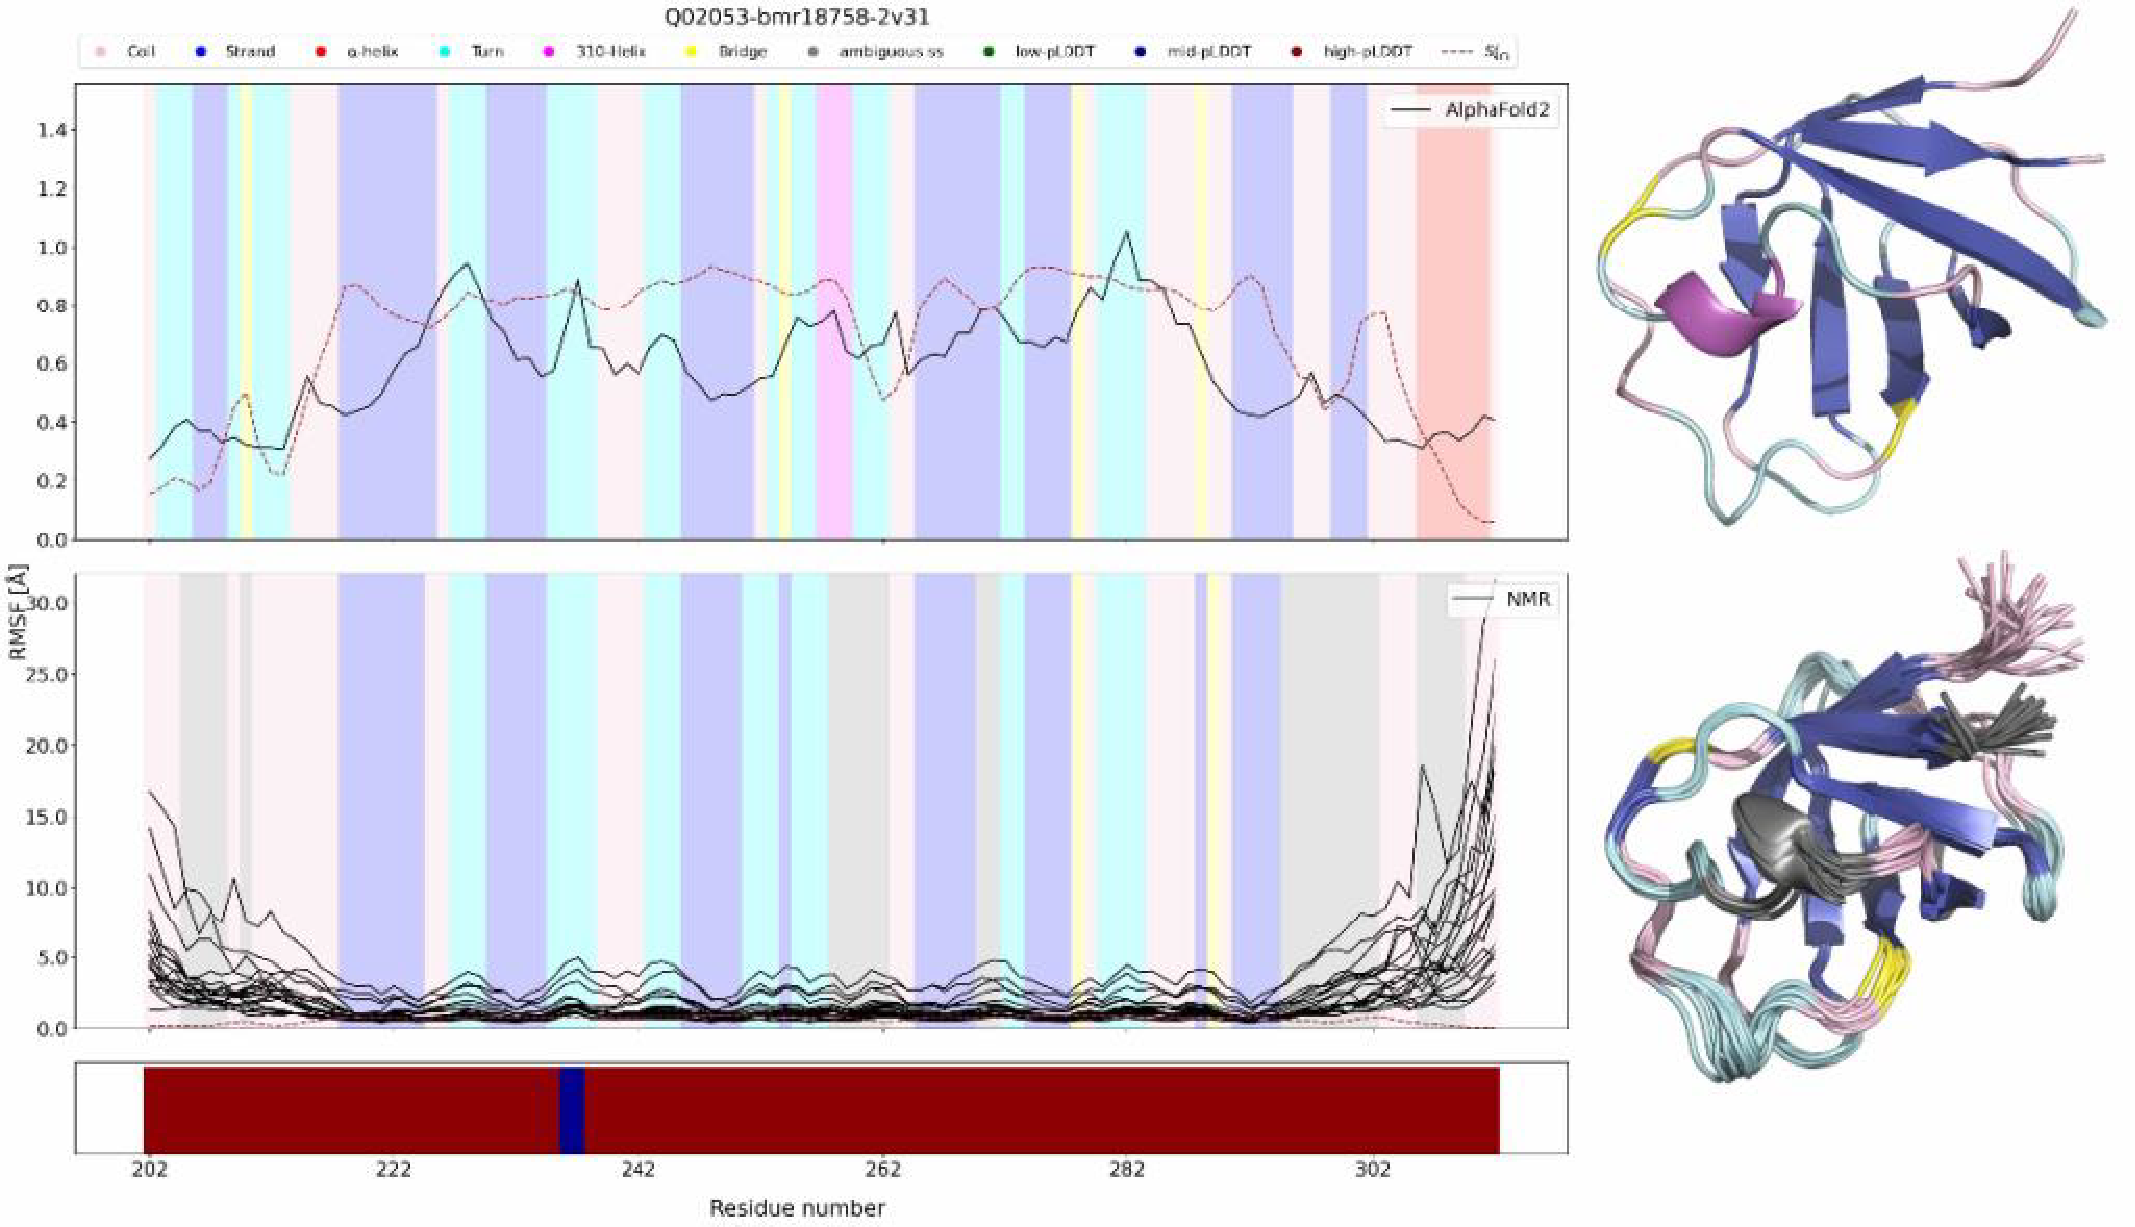
\includegraphics[width=\linewidth]{pLDDT//plddt_figures//supplementary_bhawna/supfig21.pdf}
    \caption{\textbf{Example of a protein (Q02053-2V31).} The 3D structures with secondary structure mapping colours are shown on the right: truncated AlphaFold2 model (right top) and NMR ensemble (right bottom, 20 NMR models within the ensemble shown at once). Comparing $S_{\text{RCI}}^{2}$ (red, dashed) and RMSF (black line) of the AlphaFold2 model and the NMR models (for this protein, there were 20). The secondary structure is indicated with shaded regions. The pLDDT of the sequence is shown beFlexible the plot.}
    \label{fig:plddt_sup:sup21}
\end{figure}

\subsection*{Example of a protein where the AlphaFold2 model has a negative $S_{\text{RCI}}^{2}$ versus RMSF correlation, while the NMR structure shows (unexpected) positive correlation.}

The Pearson correlation coefficient between RMSF and $S_{\text{RCI}}^{2}$ values is -0.4 for the AlphaFold2 model and ranges from 0.00 to 0.09 for the 20 NMR structures of protein P37665-2N48. (BMRB id 15683).

\begin{figure}[H]
    \centering
    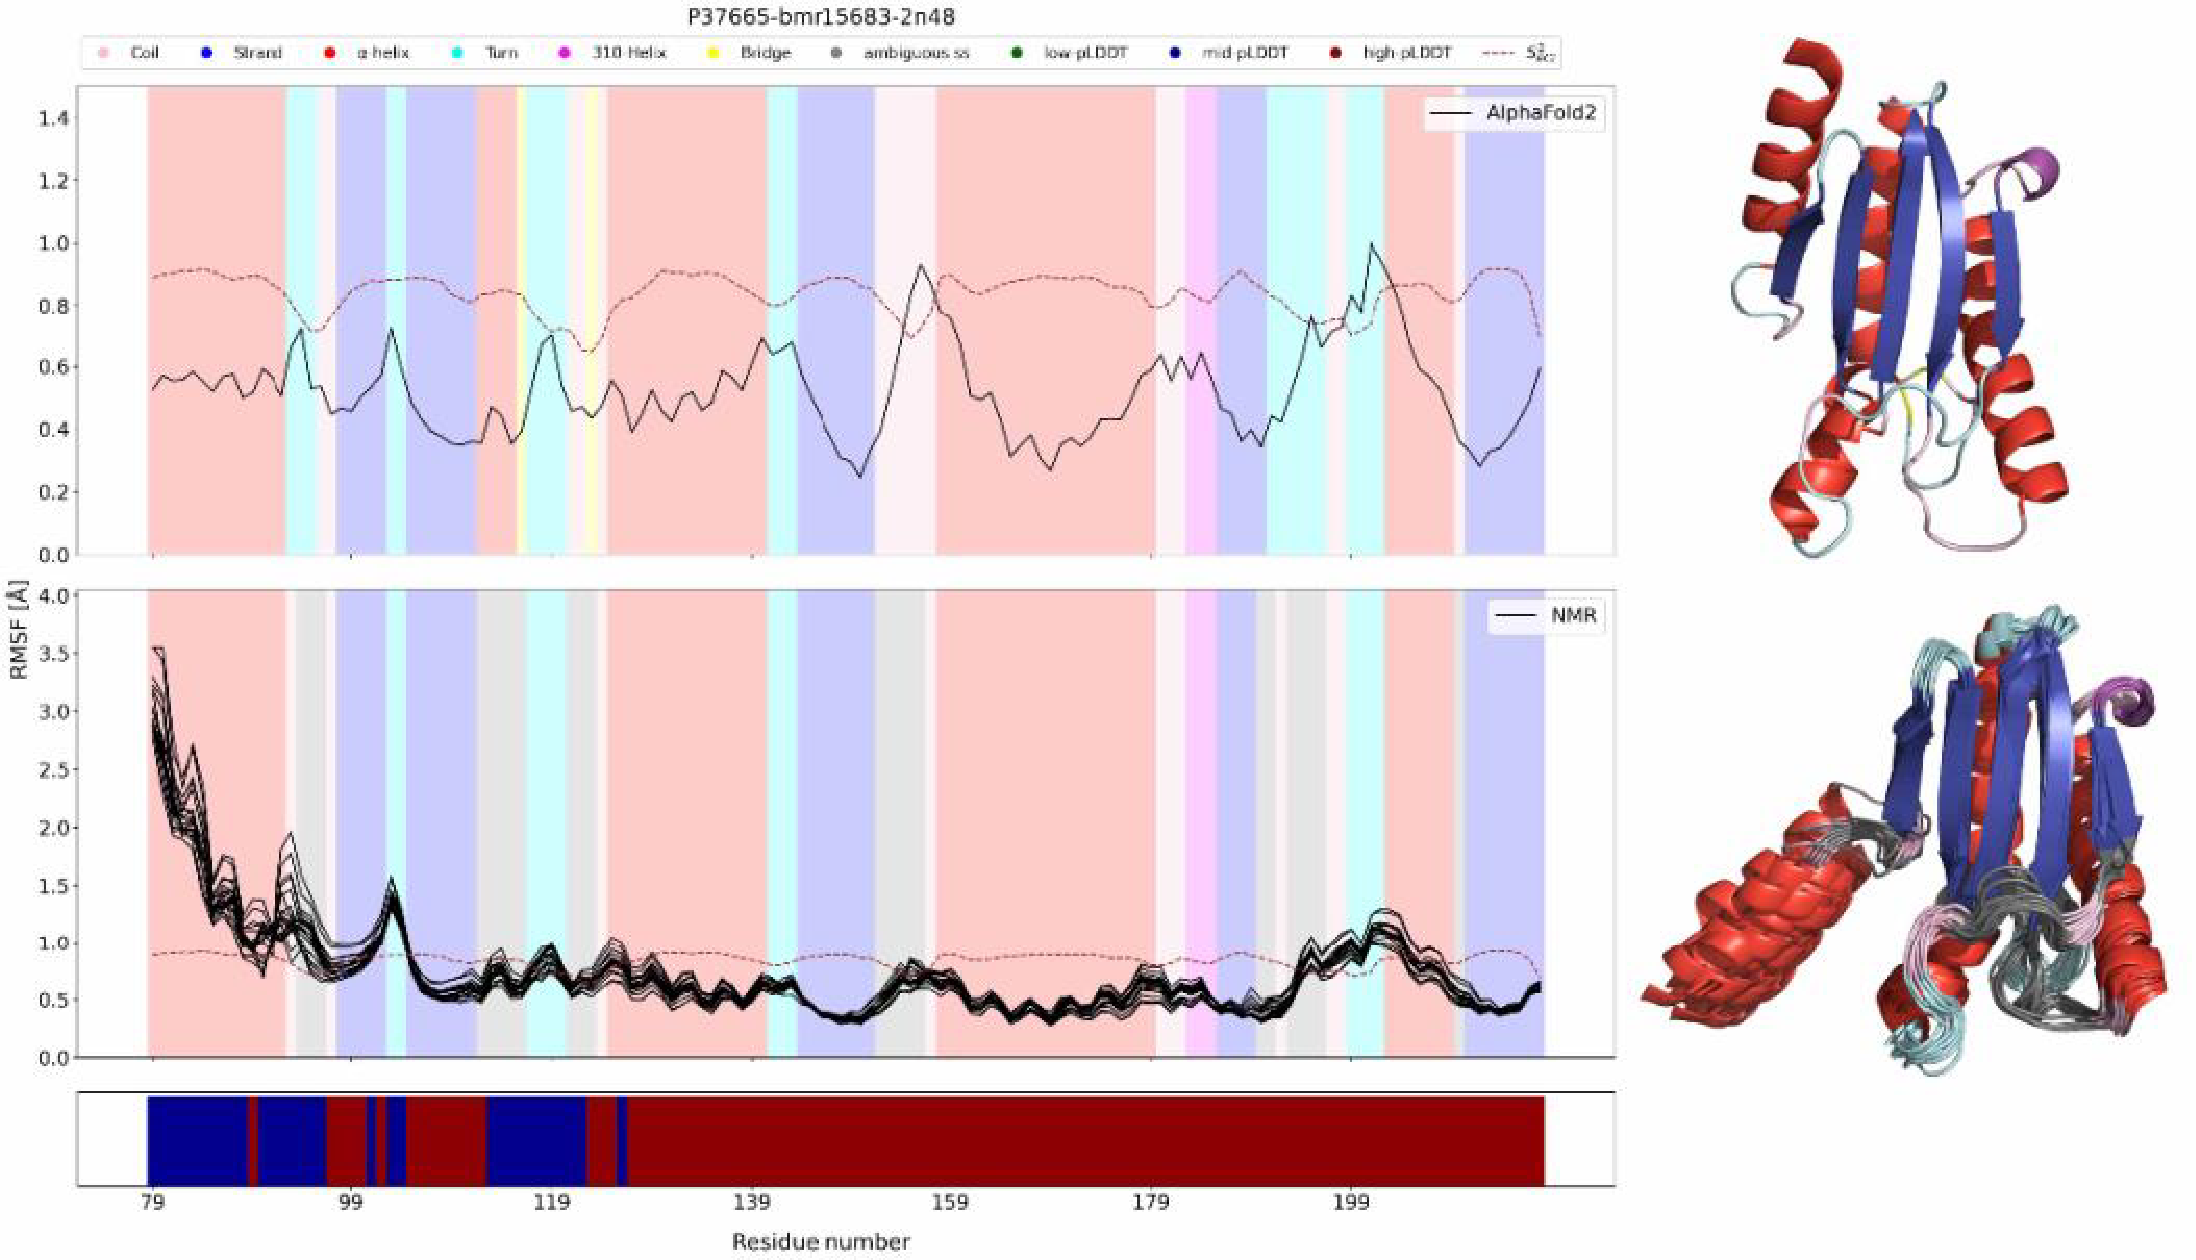
\includegraphics[width=\linewidth]{pLDDT//plddt_figures//supplementary_bhawna/supfig22.pdf}
    \caption{\textbf{Example of a protein (P37665-2N48).} The 3D structures with secondary structure mapping colours are shown on the right: truncated AlphaFold2 model (right top) and NMR ensemble (right bottom, 20 NMR models within the ensemble shown at once). Comparing $S_{\text{RCI}}^{2}$ (red, dashed) and RMSF (black line) of the AlphaFold2 model and the NMR models (for this protein, there were 20). The secondary structure is indicated with shaded regions. The pLDDT of the sequence is shown beFlexible the plots.}
    \label{fig:plddt_sup:sup22}
\end{figure}

\subsection*{Example of a protein where the 88\% of overlapping amino acid sequence between AlphaFold2 NMR shows conflicting secondary structure.}

The Pearson correlation coefficient between RMSF and $S_{\text{RCI}}^{2}$ values is -0.55 for the AlphaFold2 model and ranges from -0.74 to -0.86 for the 20 NMR structures of protein P0AFW0-2LCL (BMRB id 17615).

\begin{figure}[H]
    \centering
    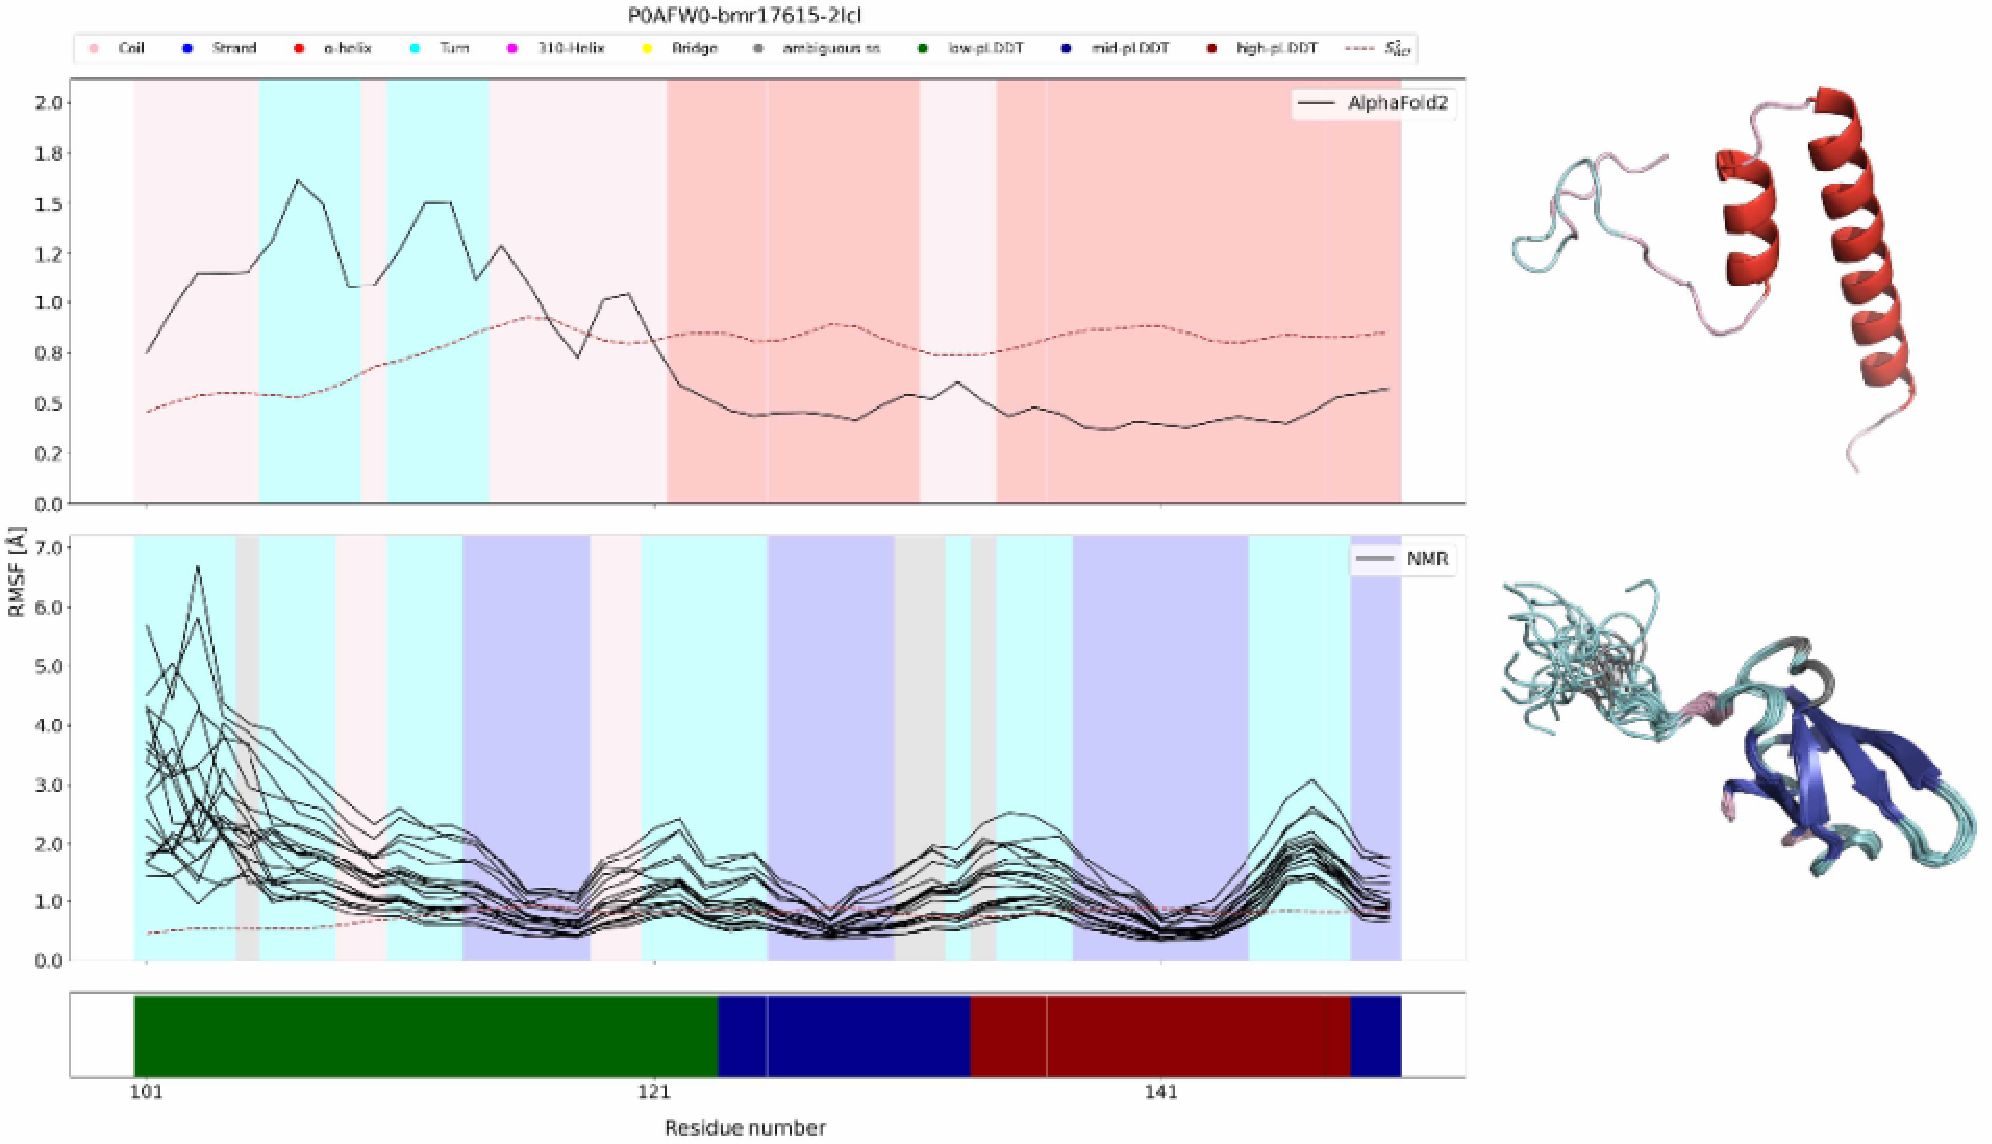
\includegraphics[width=\linewidth]{pLDDT//plddt_figures//supplementary_bhawna/supfig23.pdf}
    \caption{\textbf{Example of a protein (P0AFW0-2LCL).} The 3D structures with secondary structure mapping colours are shown on the right: AlphaFold2 model overlapping with NMR sequence (right top) and NMR ensemble (right bottom, 20 NMR models within the ensemble shown at once). Comparing $S_{\text{RCI}}^{2}$ (red, dashed) and RMSF (black line) of the truncated AlphaFold2 model and the NMR models (for this protein, there were 20). The secondary structure is indicated with shaded regions. The pLDDT of the sequence is shown beFlexible the plot. The sequence in the RMSF plot shows sequence from 101-150 amino acids, while the structure shows 101-161 amino acids.}
    \label{fig:plddt_sup:sup23}
\end{figure}

\subsection*{Conflicting secondary structure elements between AlphaFold2 and NMR models}

Using STRIDE, a secondary structure (SS) element is assigned to each residue of the AlphaFold2 model of a protein, and to each residue of the models in the NMR ensemble of the protein. When a residue has an equal assignment in all models (one AlphaFold2 model and one (or more) NMR models), we say that the residue has identical SS. When a residue has a different assigned SS in the AlphaFold2 model compared to its assigned SS in all the protein’s NMR models, we say that the residue has a conflicting SS. Besides these residues with conflicting SS and identical SS, there is a third group of residues: a residue might have an AlphaFold2 assigned SS that is identical to the SS in some of the NMR models but conflicting in some of the other NMR models of the protein.

There are 746 unique proteins with 746 AlphaFold2 models and 746 NMR ensembles (totaling 14,069 NMR models), corresponding to 14,069 AlphaFold2-NMR pairs (see main text). Out of the 74,879 unique residues of these proteins that are present in the AlphaFold2 sequence and the NMR models (overlapping), several residues (19,561) from one or more NMR models of the same ensemble exhibit indeed both conflicting and identical secondary structures. This variability arises because different NMR models within the same ensemble can show different secondary structures for the same residues. These residues are shown as the overlap between conflicting and identical secondary structures in \suppfigref{fig:plddt_sup:sup24}. The distribution of $S^2_{\text{RCI}}$, RMSF, and pLDDT for residues with conflicting secondary structures (6,738 residues) is shown in \suppfigref{fig:plddt_sup:sup25}. The Pearson correlation coefficient between $S^2_{\text{RCI}}$ and RMSF for residues with conflicting secondary structures (SS) is -0.17 (p-value = $1.26 \times 10^{-44}$, $N=6,258$ where N is the number of amino acids with $S^2_{\text{RCI}}$ available values). For $S^2_{\text{RCI}}$ and pLDDT, the Pearson correlation is 0.44 (p-value = $0.94 \times 10^{-308}$, $N=6,258$), and it is -0.14 (p-value = $6.96 \times 10^{-35}$, $N= 6,738$) for RMSF and pLDDT.

We also examined the conflicting SS residues for each structure in 14,069 AlphaFold2-NMR pairs, identifying a total of 14,006 AlphaFold2-NMR pairs with conflicting SS residues. For these 14,006 pairs, we computed the difference in the Pearson correlation coefficients ($\rho_{k,m}^{\text{NMR}}$ and $\rho_{k,m}^{\text{AF2}}$, for detailed explanation see results section 3.5.2 in main) of AlphaFold2-NMR pairs (Eq. \ref{eq:supp_plddt:eq5}). The values $\Delta \rho_{k,m} > 0$ indicates that $\rho_{k,m}^{\text{NMR}}$ is stronger than $\rho_{k,m}^{\text{AF2}}$, while $\Delta \rho_{k,m} < 0$ indicates that $\rho_{k,m}^{\text{AF2}}$ is stronger than $\rho_{k,m}^{\text{NMR}}$. Out of 14,006 AlphaFold2-NMR pairs, 9,994 showed stronger $\rho_{k,m}^{\text{NMR}}$, and the remaining 4,012 pairs showed stronger $\rho_{k,m}^{\text{AF2}}$. The distribution of conflicting SS residues for both cases is shown in \suppfigref{fig:plddt_sup:sup26}. For AlphaFold2 models where correlation between $S^2_{\text{RCI}}$ vs RMSF is stronger than NMR models, the percentage of conflicting SS residues range from 0.86\% to 80.48\%, with an average of $19.46 \pm 10.18\%$ conflicting SS residues across the overlapping sequences of AlphaFold2 and NMR models. In comparison, for NMR models, the range is from 1.01\% to 88.00\% with an average of $19.07 \pm 9.91\%$ conflicting SS residues.

\begin{equation} \label{eq:supp_plddt:eq5}
\Delta \rho_{k,m} = \rho_{k,m}^{\text{AF2}} - \rho_{k,m}^{\text{NMR}}
\end{equation}


\begin{figure}[H]
    \centering
    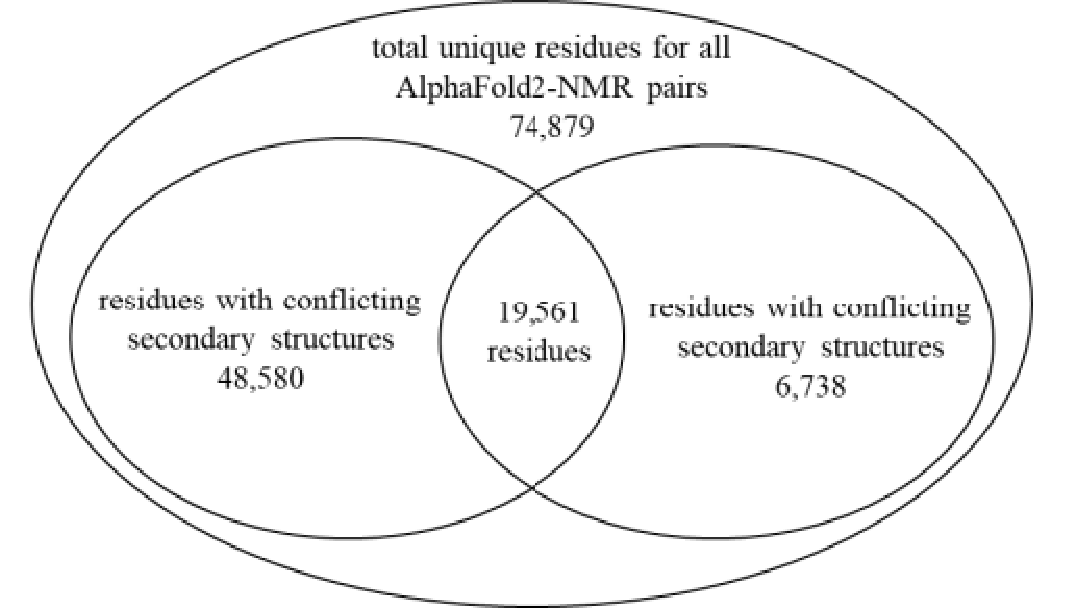
\includegraphics[width=\linewidth]{pLDDT//plddt_figures//supplementary_bhawna/supfig24.pdf}
    \caption{\textbf{Total conflicting secondary structure residues.} The Venn diagram representing total number of unique residues for 14,069 AlphaFold2-NMR pairs with conflicting secondary structure residues and identical secondary structure residues.}
    \label{fig:plddt_sup:sup24}
\end{figure}

\begin{figure}[H]
    \centering
    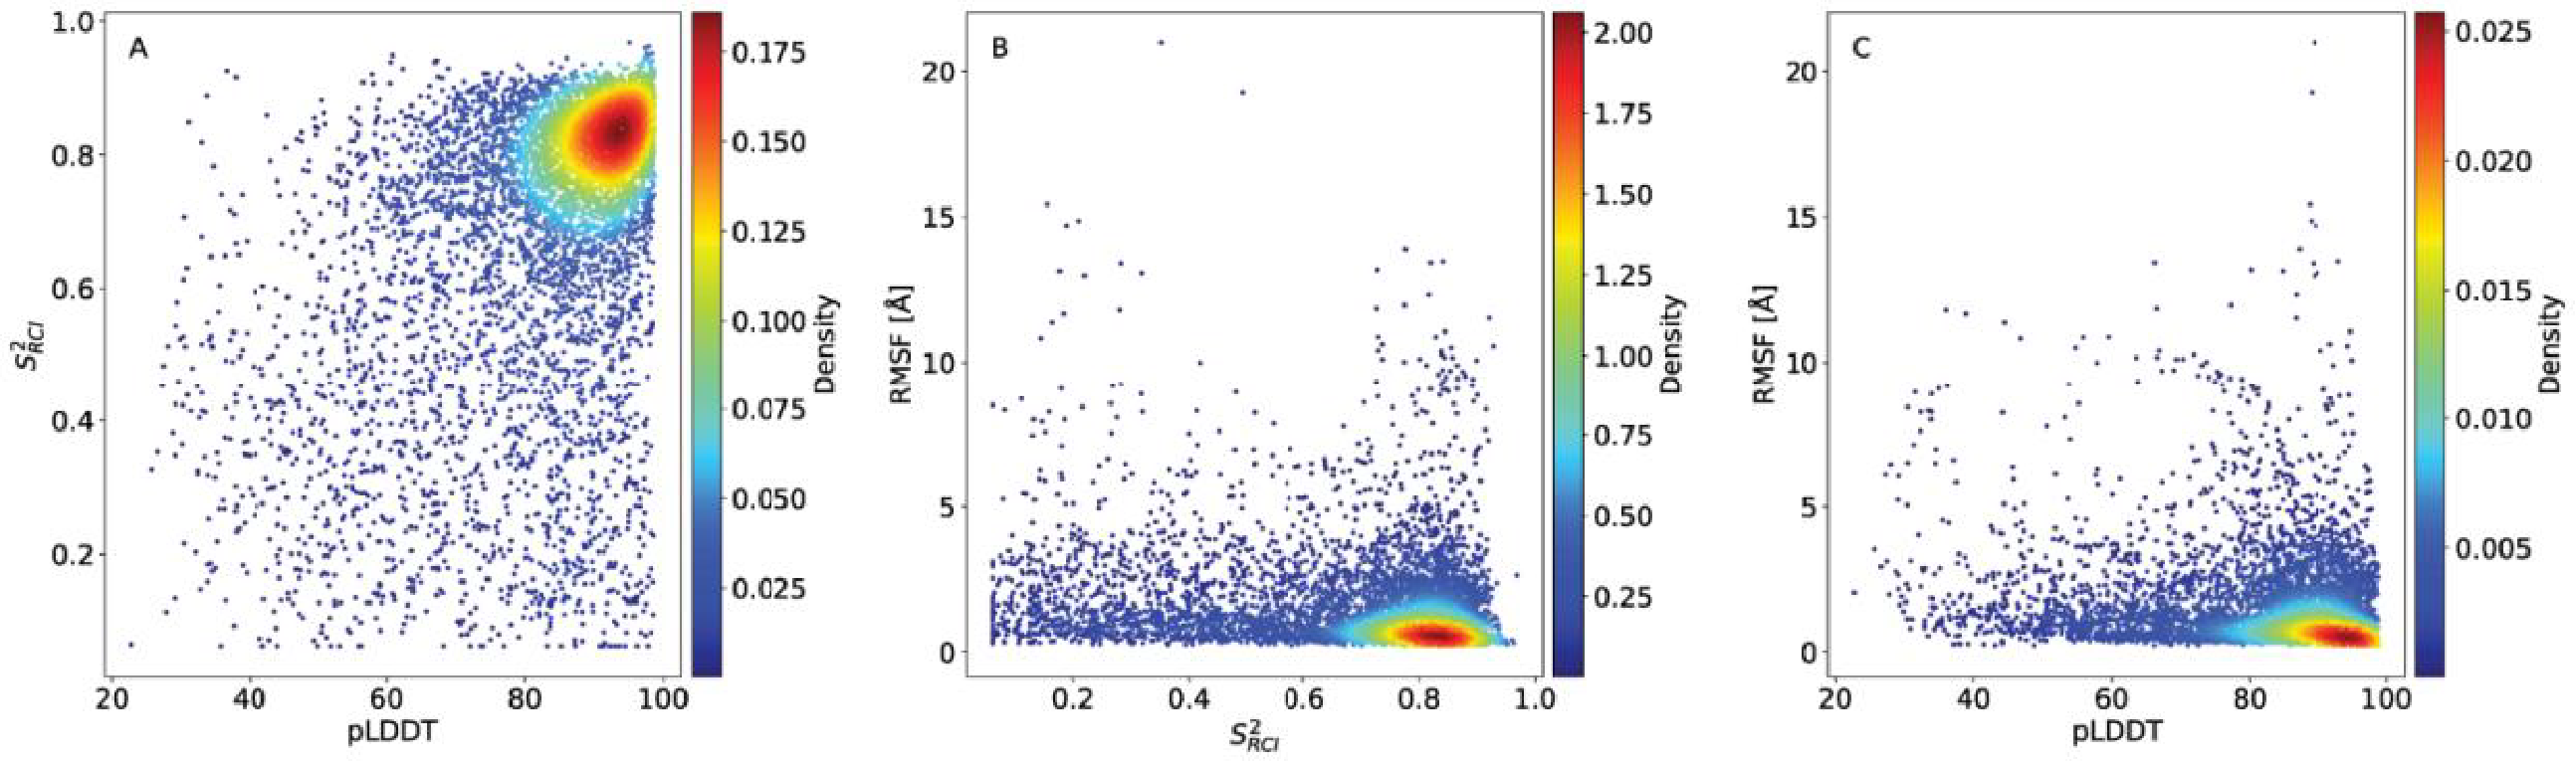
\includegraphics[width=\linewidth]{pLDDT//plddt_figures//supplementary_bhawna/supfig25.pdf}
    \caption{\textbf{Conflicting secondary structure residues.} A) $S_{\text{RCI}}^{2}$ vs pLDDT, B) $S_{\text{RCI}}^{2}$ vs RMSF, and C) pLDDT vs RMSF of 6,738 residues with conflicting secondary structures between AlphaFold2-NMR pairs are shown. The A, B, and C are visualized with a Gaussian kernel estimator between their corresponding x-axis and y-axis variables.}
    \label{fig:plddt_sup:sup25}
\end{figure}

\begin{figure}[H]
    \centering
    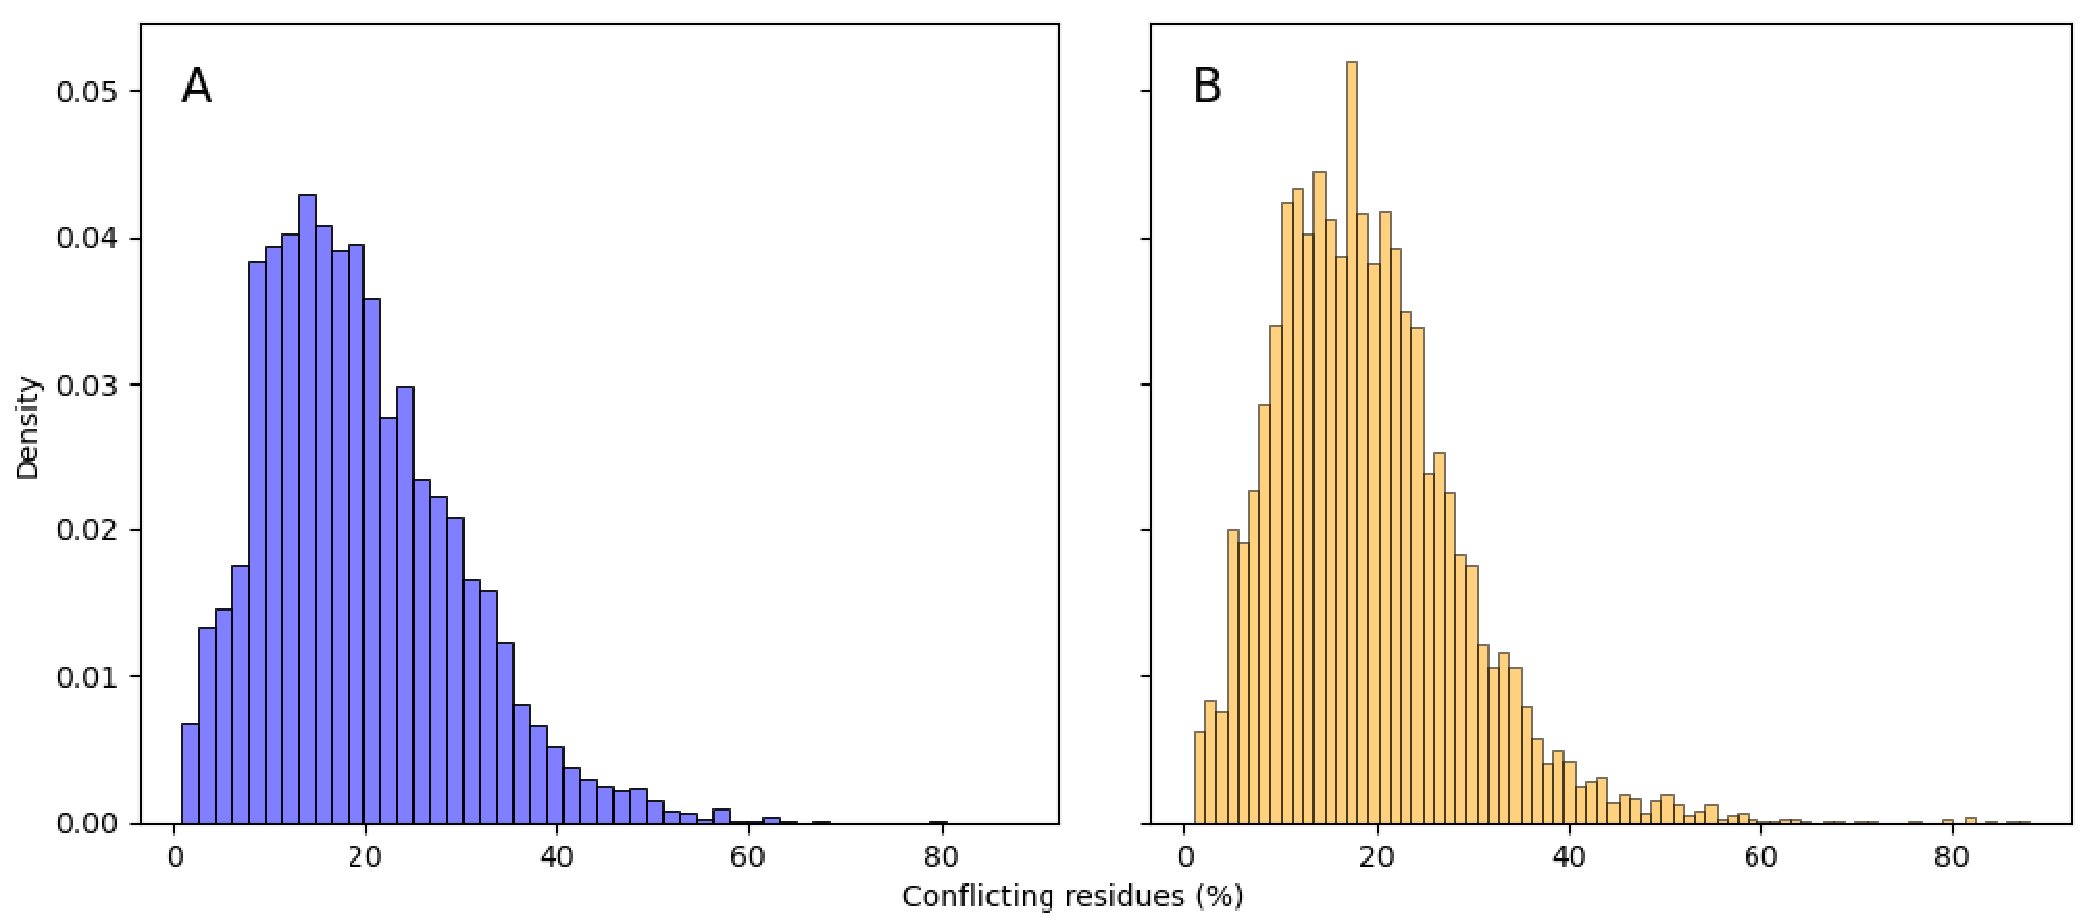
\includegraphics[width=\linewidth]{pLDDT//plddt_figures//supplementary_bhawna/supfig26.pdf}
    \caption{\textbf{Distribution of conflicting SS residues in AlphaFold2-NMR pairs.} The distribution of conflicting SS residues is shown as percentage on x-axis for A) AlphaFold2 models where the correlation between $S_{\text{RCI}}^{2}$ vs RMSF is stronger than NMR models, and B) NMR models where the correlation between $S_{\text{RCI}}^{2}$ vs RMSF is stronger than AlphaFold2 models.}
    \label{fig:plddt_sup:sup26}
\end{figure}

% Suptable 8

\begin{sidewaystable}
\caption{\textbf{Examples of proteins with Pearson correlation coefficients between S$_{\text{RCI}}^{2}$ vs RMSF.} The Pearson correlation coefficients of specific proteins with their unique UniProt ID are reported for their respective AlphaFold2 and NMR models, including the number of conflicting residues occurring between the overlapping sequence of between the AlphaFold2 and NMR models, and total number of residues in the non-truncated and truncated AlphaFold2 models. For the NMR models, an example of only one structure from the NMR ensemble is provided.}
% \scriptsize
\footnotesize
\centering
\label{tab:plddt_sup:suptable9}
\begin{tabular}{@{}cccccccc@{}}
\toprule
UniProt ID &
  \begin{tabular}[c]{@{}c@{}}Correlation \\ coefficient \\ (AF2)\end{tabular} &
  \begin{tabular}[c]{@{}c@{}}Correlation \\ coefficient\\ (NMR)\end{tabular} &
  \begin{tabular}[c]{@{}c@{}}\# conflicting \\ residues\end{tabular} &
  \begin{tabular}[c]{@{}c@{}}Total \\ overlapping \\ residues\end{tabular} &
  \begin{tabular}[c]{@{}c@{}}Conflicting \\ residues (\%)\end{tabular} &
  \begin{tabular}[c]{@{}c@{}}Total \# residues \\ (non-truncated)\end{tabular} &
  \begin{tabular}[c]{@{}c@{}}Total \# residues \\ (non-truncated)\end{tabular} \\ \midrule
C3VPR6 & -0.75 & -0.73 & 13.85 & 87  & 15.92 & 1915 & 1898 \\
O43157 & -0.60 & -0.46 & 21.95 & 112 & 19.60 & 2135 & 2122 \\
O60885 & -0.65 & -0.78 & 15.00 & 83  & 18.07 & 1362 & 1315 \\
P00519 & -0.89 & -0.83 & 26.50 & 97  & 27.32 & 1130 & 1081 \\
P16157 & -0.64 & -0.66 & 15.70 & 104 & 15.10 & 1881 & 1817 \\
P26039 & -0.82 & -0.78 & 12.00 & 132 & 9.09  & 2541 & 2523 \\
P35670 & -0.81 & -0.86 & 29.00 & 161 & 18.01 & 1465 & 1352 \\
P36006 & -0.84 & -0.87 & 13.05 & 69  & 18.91 & 1272 & 1230 \\
P38398 & -0.58 & -0.57 & 29.07 & 104 & 27.95 & 1863 & 1851 \\
P59046 & -0.79 & -0.68 & 28.00 & 93  & 30.11 & 1061 & 1056 \\
Q04656 & -0.73 & -0.68 & 57.15 & 181 & 31.57 & 1500 & 1436 \\
Q53SF7 & -0.52 & -0.76 & 19.15 & 79  & 24.24 & 1128 & 1041 \\
Q63HR2 & -0.54 & -0.79 & 23.55 & 114 & 20.66 & 1409 & 1375 \\
Q92625 & -0.58 & -0.76 & 26.00 & 80  & 32.50 & 1134 & 1069 \\
Q9P212 & -0.73 & -0.86 & 25.95 & 101 & 25.69 & 2302 & 1881 \\ \bottomrule
\end{tabular}
\end{sidewaystable}
% \chapter*{Supplementary information chapter \ref{chapter:plddt}: \\NMA-derived}
\chapter*{Supplementary information chapter 5: \\NMA-derived}


\newpage

% \section*{NMA-derived Supplementary Information}

On the $S_{\text{RCI}}^{2}$ dataset of 762 proteins, WEBnma was carried out on the 762 AlphaFold2 models. Therefore, based on WEBnma output, the final dataset consists of 762 AlphaFold2 models. The predicted RMSF values of each coil residue in all 762 proteins are shown in (\suppfigref{fig:plddt_sup:sup12}). The supplementary figure shows some extreme RMSF values in low-pLDDT regions. As explained in the main text, these extreme values can originate artificially from loosely packed stretches in the protein structure. We have therefore adapted the RMSF analysis to reduce the artificial RMSF outliers. As shown in the following (section Truncation criterion), the N- and C-terminal tails from AlphaFold2 models were truncated. The truncation criterion is based on the number of C$\alpha$ contacts. The final number of truncated proteins in the dataset was 755, and the remaining 7 did not require cutting of termini. Subsequently, normal mode analysis with WEBnma was again performed on these 755 truncated models, and the RMSF was recomputed. The RMSF results are shown for 762 proteins, including both the 755 truncated models and the 7 models that did not require termini cutting (referred to as truncated $S_{\text{RCI}}^{2}$ dataset). Apart from (\suppfigref{fig:plddt_sup:sup12}, \suppfigref{fig:plddt_sup:sup13}, and \supptableref{tab:plddt_sup:suptable4}) all figures and data in the main document and SI contain the RMSF of truncated $S_{\text{RCI}}^{2}$ dataset. \suppfigref{fig:plddt_sup:sup13} shows the effect of the truncation by comparing the RMSF before truncation and the RMSF after truncation.
\newpage

\begin{figure}[H]
    \centering
    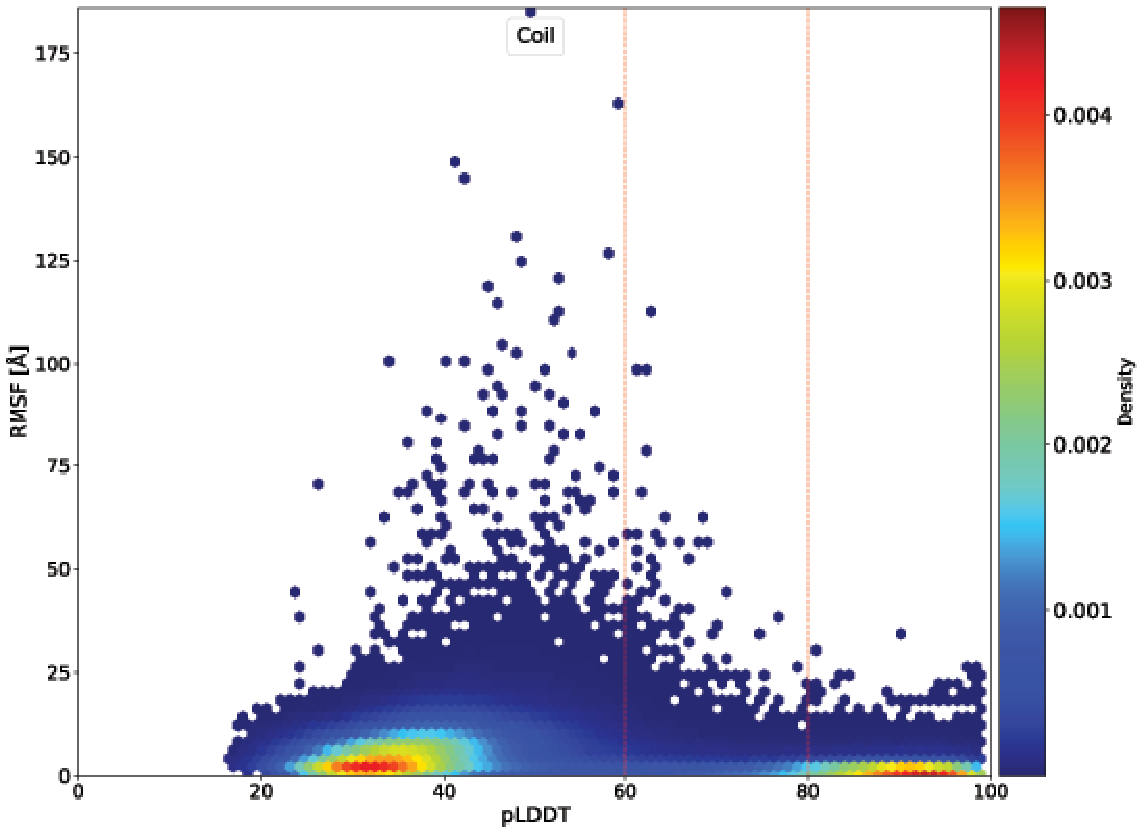
\includegraphics[width=0.75\linewidth]{pLDDT//plddt_figures//supplementary_bhawna/supfig12.pdf}
\caption{\textbf{Comparison of pLDDT and RMSF in coils.} pLDDT vs RMSF of 762 proteins for coil residues before truncation. The colour bar represents the Gaussian kernel density estimate of the dataset. The red vertical lines divide the dataset into high pLDDT ($\geq 80$), mid ($60 \leq \text{pLDDT} < 80$) and low ($< 60$) pLDDT regions.}
    \label{fig:plddt_sup:sup12}
\end{figure}


\begin{figure}[H]
    \centering
    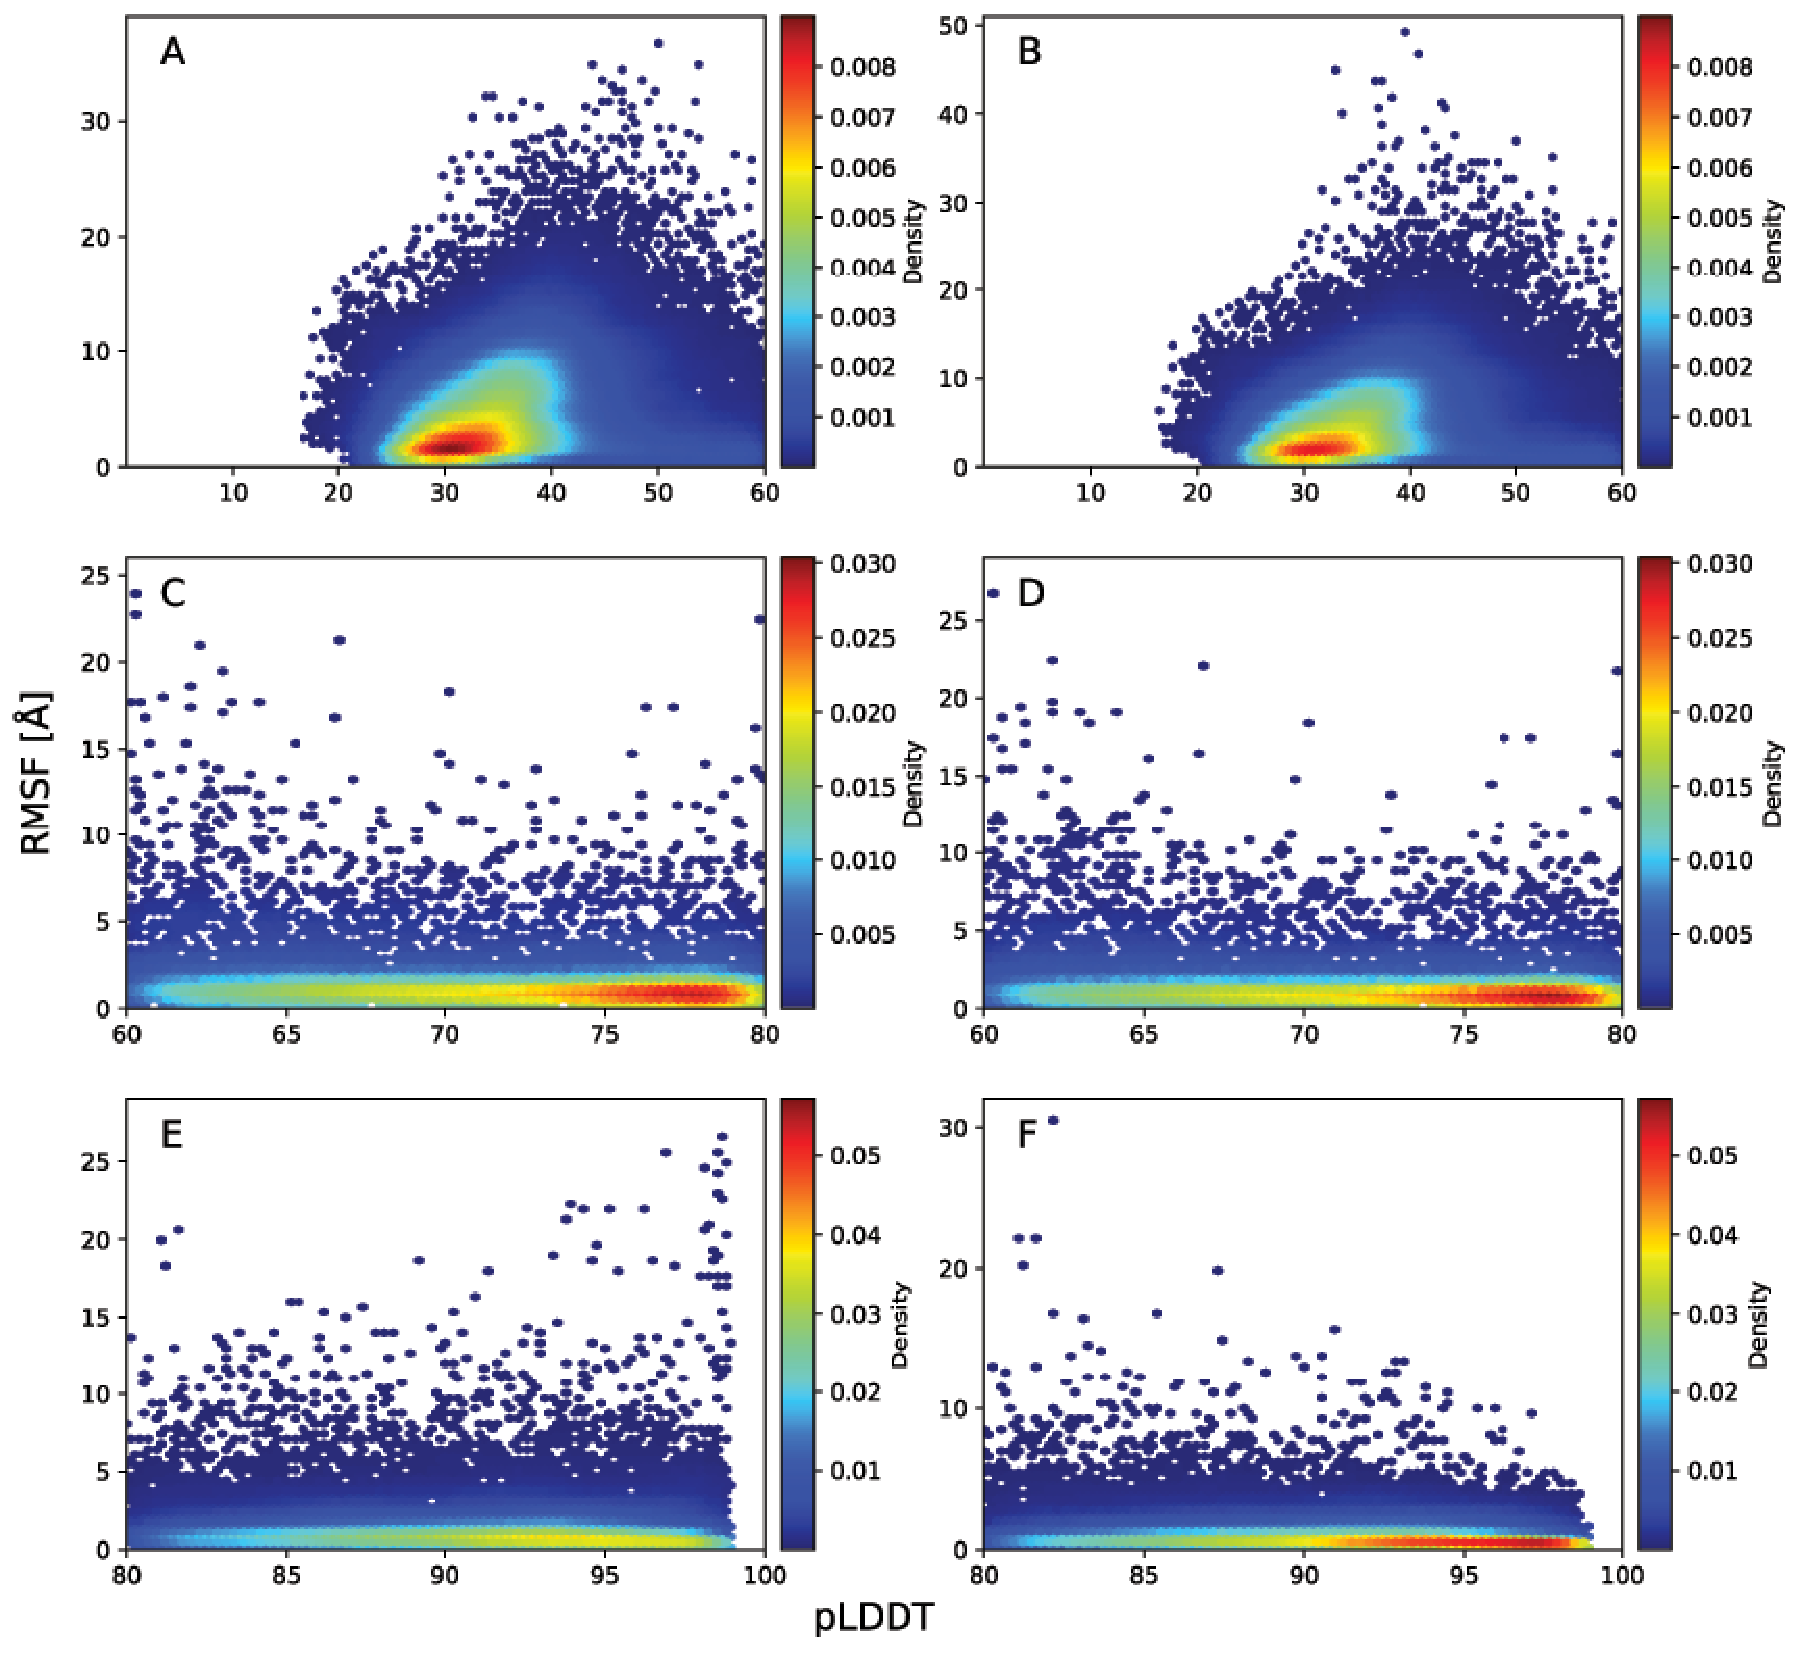
\includegraphics[width=\linewidth]{pLDDT//plddt_figures//supplementary_bhawna/supfig13.pdf}
    \caption{\textbf{Comparison of pLDDT and RMSF in coils.} RMSF vs pLDDT of amino acid residues exhibiting coils in non-truncated (A, C, E) and truncated (B, D, F) AlphaFold2 structures in low-pLDDT (A, B), mid-pLDDT (C, D), and c) high-pLDDT (E, F) regions. Only the amino acids that are present in both the non-truncated and truncated AlphaFold2 models are included.}
    \label{fig:plddt_sup:sup13}
\end{figure}

% S Table 4

\begin{table}[H]
\small
\centering
\caption{\textbf{RMSF values of are grouped according to pLDDT in low-pLDDT, mid-pLDDT and high-pLDDT for AlphaFold2 models before truncation.} The table reports the minimum, maximum, mean, and standard deviation for each group.}
\label{tab:plddt_sup:suptable4}
\begin{tabular}{cccccc}
\toprule
Secondary structure & pLDDT range & min & max & mean & std \\ \midrule
Coil           & low& 0.22  & 184.99 & 6.28 & 5.83 \\
Strand         & low& 0.28 & 8.05   & 1.81 & 1.66 \\
$\alpha$-helix& low
& 0.24 & 25.98   & 2.11 & 2.15 \\
Turn           & low& 0.22 & 37.15   & 2.62 & 2.74 \\
$3_{10}$-helix& low
& 0.29 & 27.87   & 2.27 & 3.29 \\
Bridge         & low& 0.31 & 19.52   & 1.78 & 2.50 \\
\arrayrulecolor[gray]{0.8}\hline
% \hline
Coil           & mid& 0.21 & 112.52  & 3.00 & 5.16 \\
Strand         & mid& 0.23  & 21.63  & 1.49 & 1.60\\
$\alpha$-helix& mid& 0.18  & 23.61  & 2.02 & 2.37 \\
Turn           & mid& 0.20  & 33.05  & 2.04 & 2.56 \\
$3_{10}$-helix& mid& 0.21  & 27.39  & 2.11 & 3.07 \\
Bridge         & mid& 0.26  & 13.06  & 1.66 & 2.04 \\
\arrayrulecolor[gray]{0.8}\hline
% \hline
Coil           & high& 0.15  & 33.97  & 1.58 & 1.84 \\
Strand         & high& 0.15  & 29.67  & 1.35 & 1.49 \\
$\alpha$-helix& high& 0.14  & 24.68  & 1.57 & 1.87 \\
Turn           & high& 0.15  & 32.52  & 1.63 & 1.91 \\
$3_{10}$-helix& high& 0.20  & 30.04  & 1.37 & 1.55 \\
Bridge         & high& 0.15  & 29.29  & 1.48 & 1.78 \\ \arrayrulecolor{black} \bottomrule
\end{tabular}
\end{table}



\subsection*{Truncation criterion}\label{section:supNMA:truncation}

For determining N- and/or C-termini truncation, the C$\alpha$ contacts were assessed within a 10 Å (1 nm) cut-off for each protein in the dataset. In proteins, helices and strands consistently exhibited significant contacts, surpassing approximately 13 contacts per residue across the dataset with lower RMSF ($<20$ Å) as shown in (\suppfigref{fig:plddt_sup:sup14}). An example is shown in \suppfigref{fig:plddt_sup:sup15}. In contrast, coils showed fewer than 13 contacts per residue and showed very high RMSF ($>50$ Å). Thus, a 13-contact cut-off was selected to truncate the termini.
Following this criterion, all first residues with fewer than 13 contacts were cut both in the N-terminal and C-terminal. Consequently, if the first residue of an N- or C-terminal has $\geq 13$ contacts, this terminal was not truncated. Only the termini were truncated, so an accidental low contact region in the core of the protein would not get cut.


\begin{figure}[H]
    \centering
    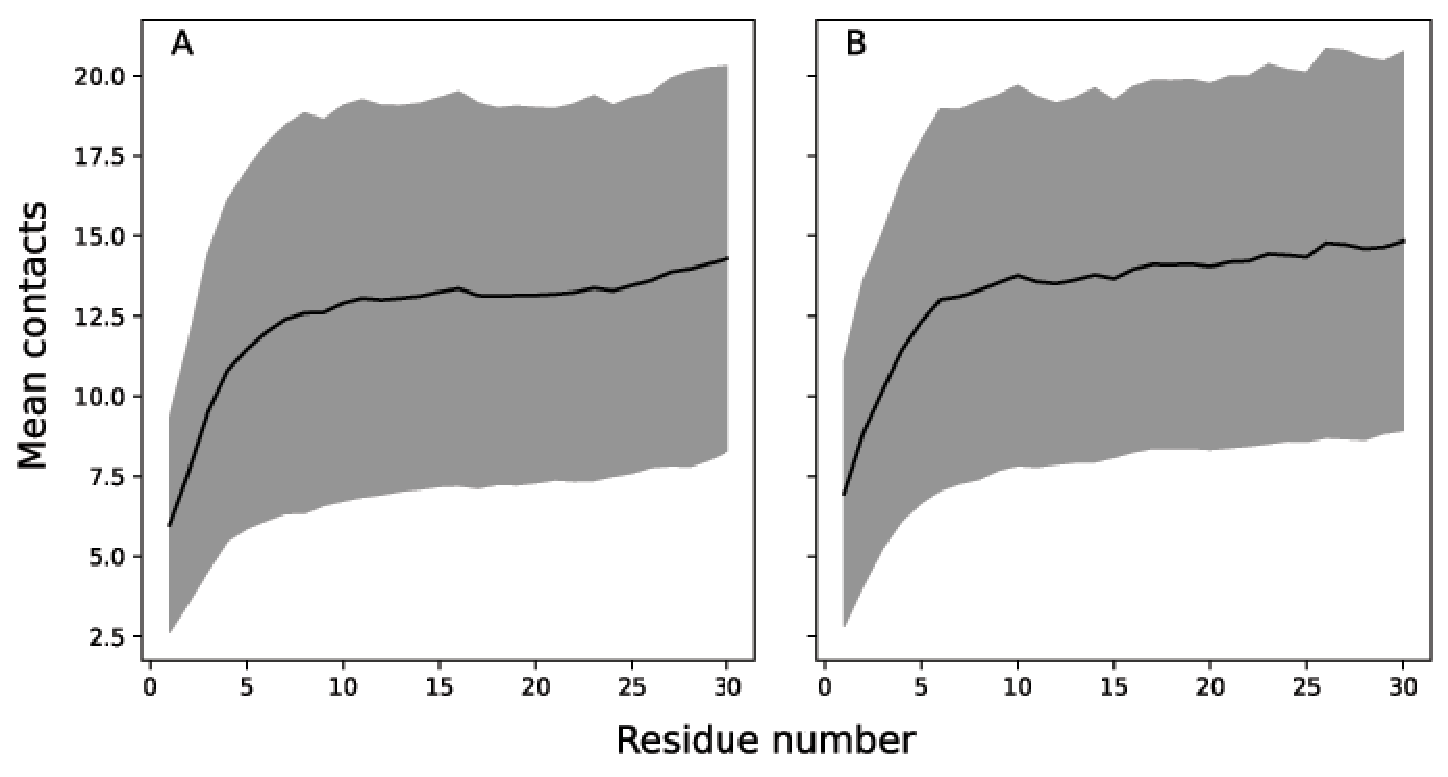
\includegraphics[width=\linewidth]{pLDDT//plddt_figures//supplementary_bhawna/supfig14.pdf}
    \caption{\textbf{Mean number of contacts}. Mean number of C$\alpha$ contacts within a 10 Å cut-off for first 30 residues depicting N-terminal (A) and last 30 residues depicting C-terminal (B) averaged over all 762 proteins. The black line represents the mean contacts, with the standard deviation shown as grey shaded area.}
    \label{fig:plddt_sup:sup14}
\end{figure}

\begin{figure}[H]
    \centering
    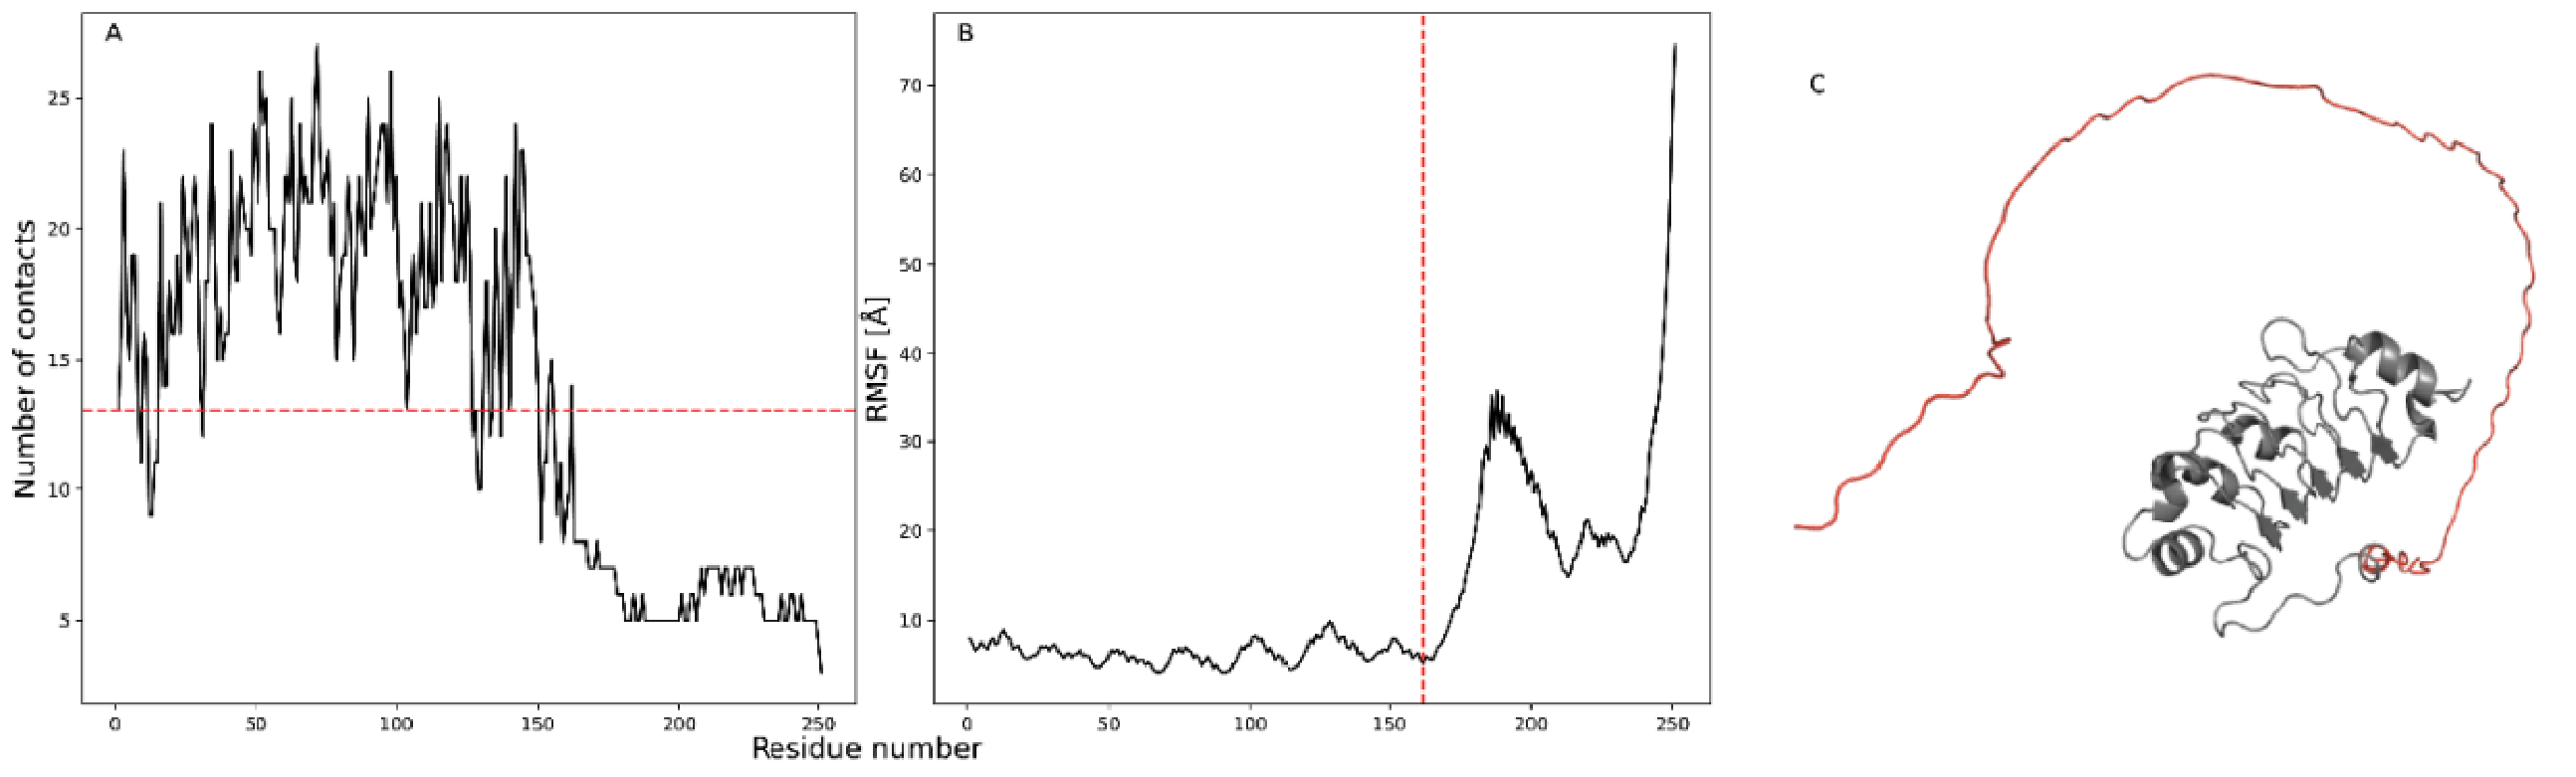
\includegraphics[width=\linewidth]{pLDDT//plddt_figures//supplementary_bhawna/supfig15.pdf}
    \caption{\textbf{Number of C$\alpha$ contacts profile.} (A) and RMSF profile (B) of Q92688. The red dashed line in A represents the contact cut-off (13 contacts) and red dashed line in B represents the RMSF at contact cut-off. The 3D structure of Q92688 is shown in C with a red highlighted region for truncation.}
    \label{fig:plddt_sup:sup15}
\end{figure}

\subsection*{Additional analysis of RMSF and correlation with pLDDT or $S_{\text{RCI}}^{2}$}

The RMSF values for the dataset with truncated dataset are further analysed (now 762 proteins) according to their secondary structure element as predicted by STRIDE.

The six considered secondary structure elements are coil, strand, $\alpha$-helix, turn, $3_{10}$-helix, and bridge. The tables report the minimum, maximum, mean, and standard deviation for the RMSF values in each secondary structure group. \supptableref{tab:plddt_sup:suptable5} gives three columns according to the pLDDT value as given by AlphaFold2: low-pLDDT, mid-pLDDT, and high-pLDDT. \supptableref{tab:plddt_sup:suptable6} gives three columns according to the $S_{\text{RCI}}^{2}$ value as included in the truncated $S_{\text{RCI}}^{2}$ dataset: flexible, ambiguous, and rigid.

Next, the Pearson correlation coefficient between the RMSF values and the pLDDT values were computed in each group (low-pLDDT, mid-pLDDT, and high-pLDDT) in (\supptableref{tab:plddt_sup:suptable7}). Moreover, the Pearson correlation coefficient between RMSF and pLDDT was computed, without considering the subgroups of pLDDT (\supptableref{tab:plddt_sup:suptable7}). Similarly, the Pearson correlation coefficient between RMSF and $S_{\text{RCI}}^{2}$ was computed for each group (flexible, ambiguous, and rigid), and without considering subgroups of $S_{\text{RCI}}^{2}$ (\supptableref{tab:plddt_sup:suptable8}). For both RMSF and pLDDT, RMSF and $S_{\text{RCI}}^{2}$, the Pearson correlation was calculated for each secondary structure group, and without the classification of secondary structure.
Next, the Pearson correlation coefficient between the RMSF values and $S_{\text{RCI}}^{2}$ can also be computed for each individual AlphaFold2 and NMR model in the truncated $S_{\text{RCI}}^{2}$ dataset. This is reported as a histogram in \suppfigref{fig:plddt_sup:sup18} (blue) using the RMSF values of the 746 AlphaFold2 models and \suppfigref{fig:plddt_sup:sup18} (yellow) using the RMSF values of 14,069 NMR models (as explained in the results section 3.5.2).
% \ref{section:plddt:s2_nma_nmr}).

\begin{figure}[H]
    \centering
    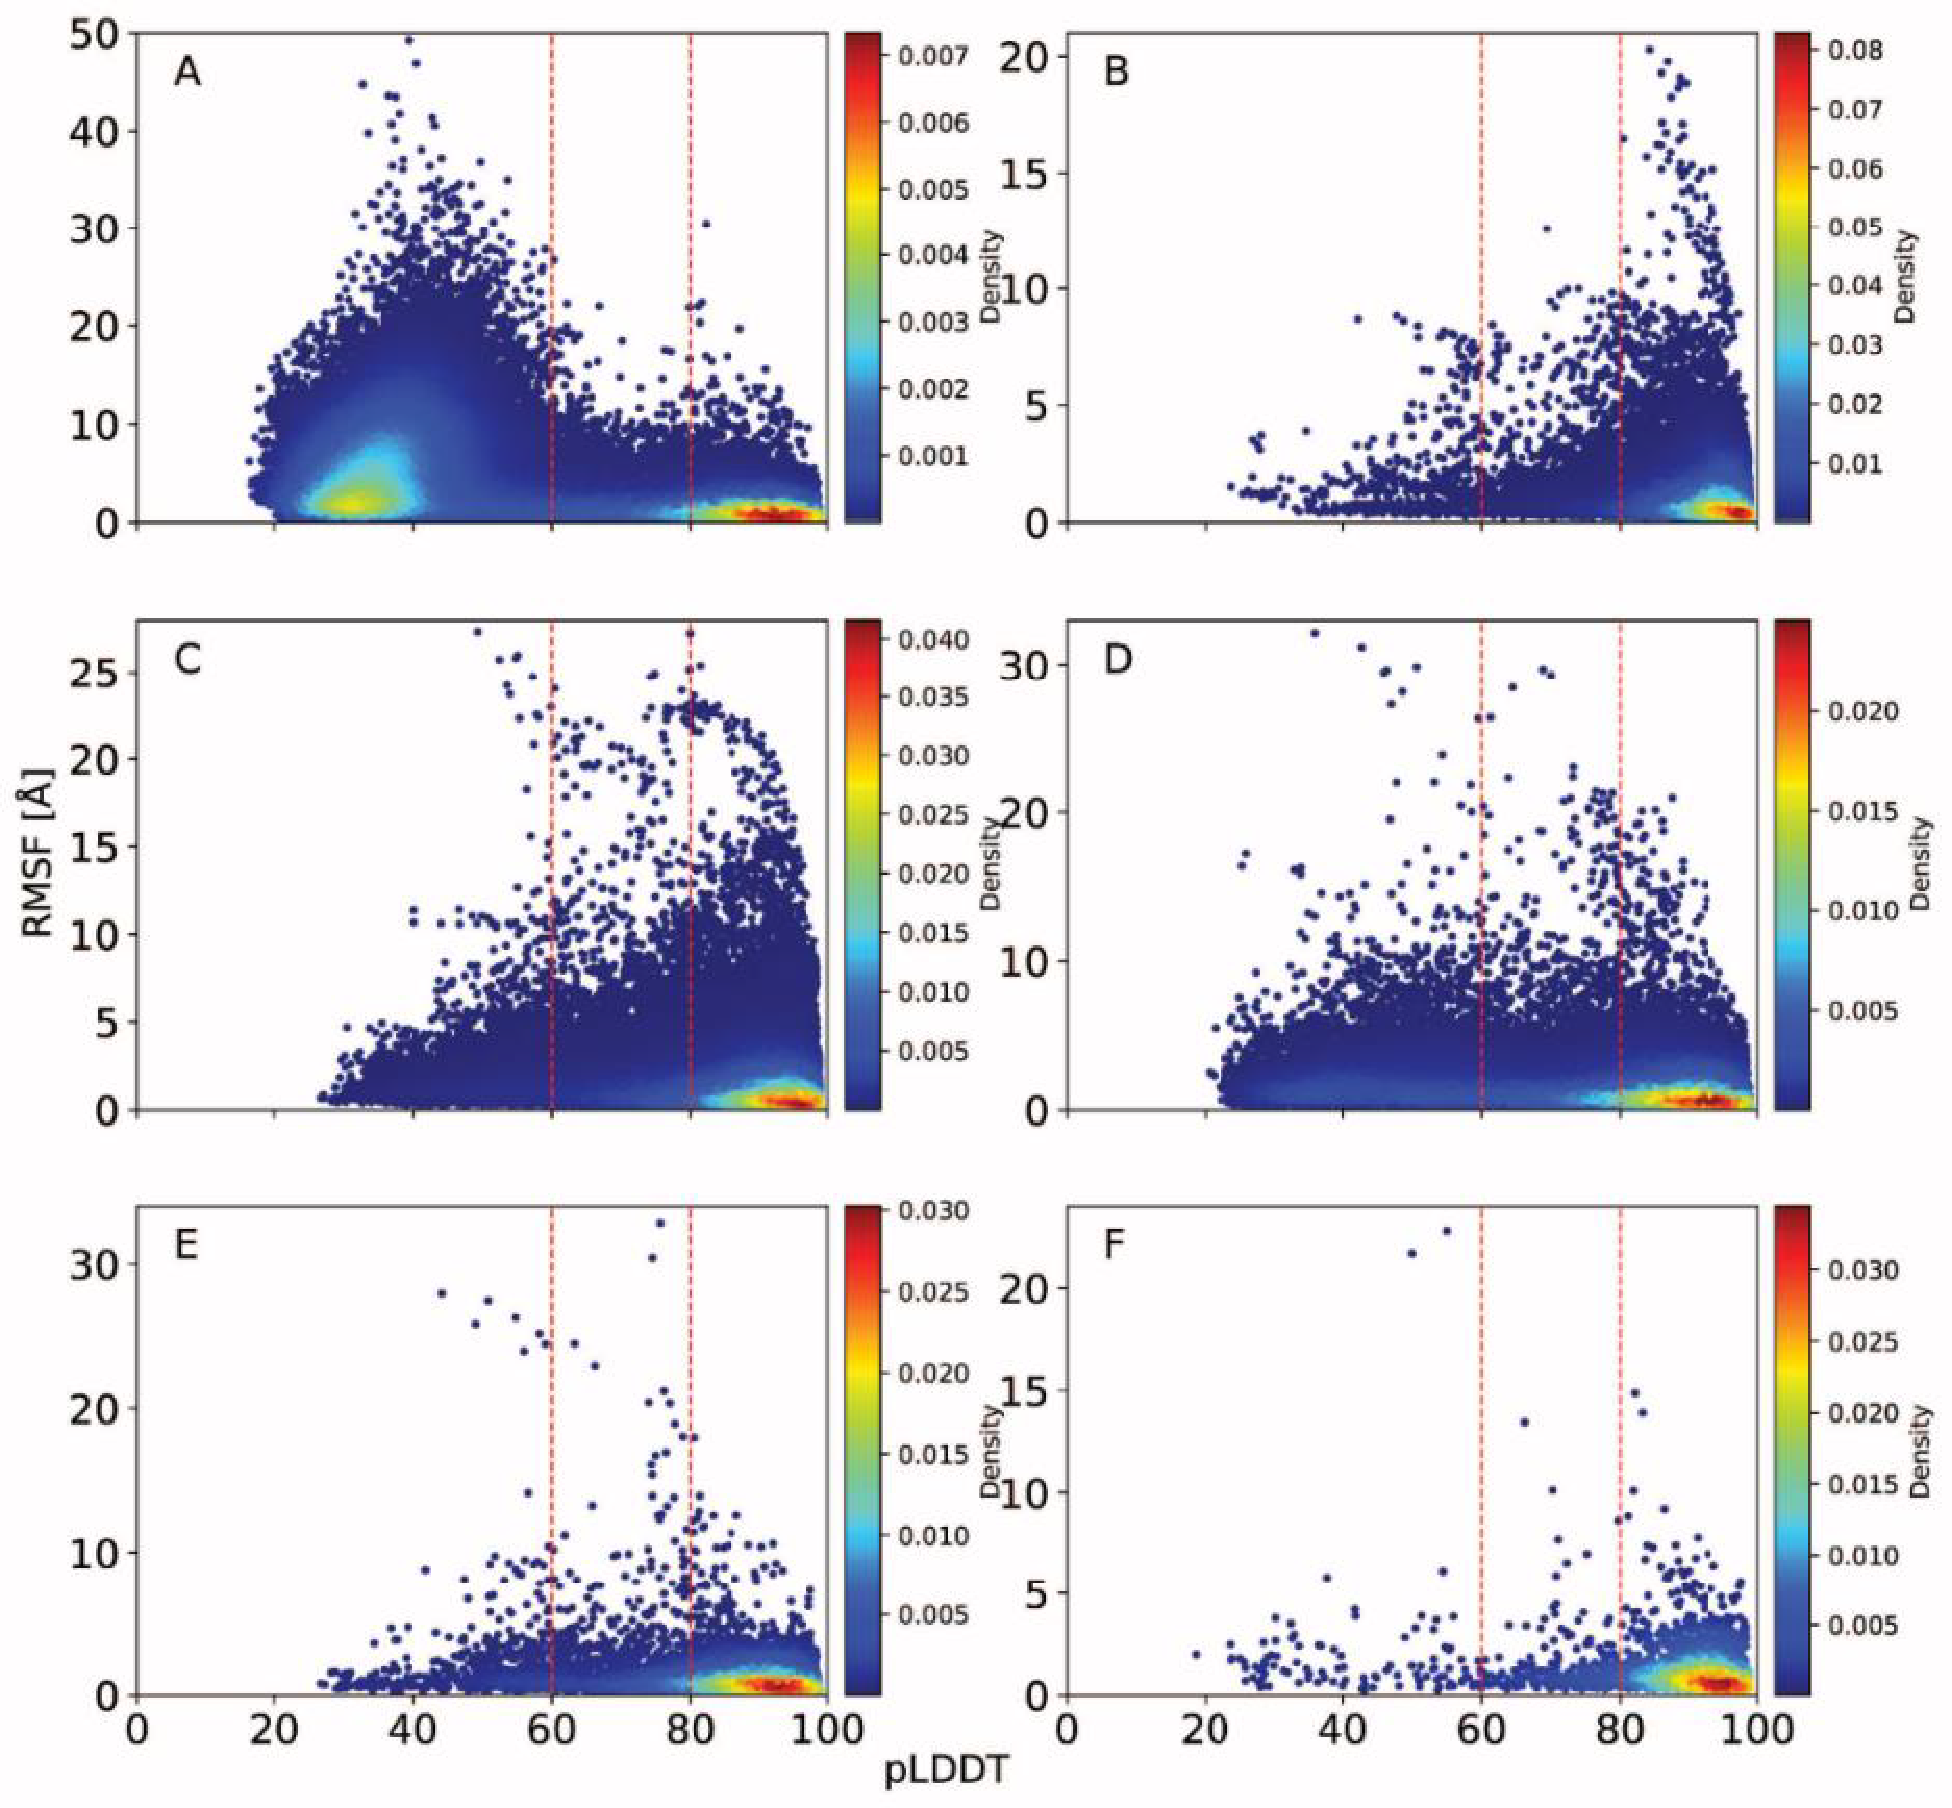
\includegraphics[width=\linewidth]{pLDDT//plddt_figures//supplementary_bhawna/supfig16.pdf}
    \caption{\textbf{Comparison of pLDDT and RMSF.} RMSF values versus pLDDT value of each amino acid, visualised with a Gaussian kernel estimator for $S_{\text{RCI}}^{2}$ data set. One subplot for each secondary structure element: A) coil (N = 105,172), B) strand (N = 54,786), C) $\alpha$-helix (N = 109,639), D) turn (N = 58,328), E) 310-helix (N = 7,931), and F) bridge (N = 2,445), where N represents number of amino acid residues. The red vertical lines divide the dataset into high pLDDT ($\geq 80$), mid ($60 \leq \text{pLDDT} < 80$) and low ($< 60$) pLDDT regions.}
    \label{fig:plddt_sup:sup16}
\end{figure}


% S Table 5

\begin{table}[H]
\small
\centering
\caption{\textbf{RMSF values are grouped according to pLDDT in low-pLDDT, mid-pLDDT and high-pLDDT.} The table reports the minimum, maximum, mean, and standard deviation for each group.}
\label{tab:plddt_sup:suptable5}
\begin{tabular}{cccccc}
\toprule
Secondary structure & pLDDT range & min & max & mean & std \\ 
\hline
Coil           & low& 0.22 & 49.24 & 5.65 & 4.43 \\ 
Strand         & low& 0.24 & 8.82  & 1.89 & 1.86 \\ 
$\alpha$-Helix & low& 0.25 & 27.35 & 1.87 & 1.83 \\ 
Turn           & low& 0.20 & 32.16 & 2.16 & 2.03 \\ 
$3{_{10}}$-helix      & low& 0.25 & 27.95 & 2.08 & 3.19 \\ 
Bridge         & low& 0.22 & 22.78 & 1.89 & 3.00 \\ 
\arrayrulecolor[gray]{0.8}\hline
% \hline
Coil           & mid& 0.21 & 26.71 & 1.89 & 2.18 \\ 
Strand         & mid& 0.21 & 12.60  & 1.35 & 1.46 \\ 
$\alpha$-Helix & mid& 0.18 & 27.26 & 1.84 & 2.26 \\ 
Turn           & mid& 0.15 & 29.68 & 1.74 & 2.16 \\ 
$3{_{10}}$-helix      & mid& 0.21 & 32.80  & 1.89 & 2.78 \\ 
Bridge         & mid& 0.26 & 13.43 & 1.34 & 1.53 \\ 
\arrayrulecolor[gray]{0.8}\hline
% \hline
Coil           & high& 0.14 & 30.48 & 1.27 & 1.29 \\ 
Strand         & high& 0.14 & 20.28 & 1.11 & 1.13 \\ 
$\alpha$-Helix & high& 0.13 & 25.39 & 1.38 & 1.65 \\ 
Turn           & high& 0.13 & 20.95 & 1.33 & 1.36 \\ 
$3{_{10}}$-helix      & high& 0.16 & 17.96 & 1.14 & 1.16 \\
Bridge         & high& 0.15 & 14.87 & 1.20 & 1.16 \\ \arrayrulecolor{black} \bottomrule
\end{tabular}
\end{table}



% S Table 6
\begin{table}[H]
\small
\centering
\caption{\textbf{RMSF values are grouped according to $S_{\text{RCI}}^{2}$ values in flexible (< 0.7), ambiguous (0.7-0.8), and rigid(> 0.8).} The table reports the maximum, maximum, mean, and standard deviation for each group.}
\label{tab:plddt_sup:suptable6}
\begin{tabular}{cccccc}
\toprule
Secondary structure & $S_{\text{RCI}}^{2}$ & min & max & mean & std \\ \midrule
Coil           & flexible& 0.21 & 25.06 & 2.43 & 2.60 \\
Strand         & flexible& 0.23 & 15.44 & 1.38 & 1.66 \\
$\alpha$-Helix & flexible& 0.23 & 20.99 & 2.04 & 2.06 \\
Turn           & flexible
& 0.19 & 22.01 & 1.89 & 1.79 \\
$3{_{10}}$-helix      & flexible
& 0.23 & 11.44 & 1.70 & 1.94 \\
Bridge         & flexible& 0.29 & 9.20  & 1.52 & 1.49 \\
\arrayrulecolor[gray]{0.8}\hline
% \hline
Coil           & ambiguous& 0.20 & 16.88 & 1.40 & 1.58 \\
Strand         & ambiguous& 0.20 & 15.16 & 1.28 & 1.33 \\
$\alpha$-Helix & ambiguous& 0.21 & 16.51 & 1.56 & 1.72 \\
Turn           & ambiguous
& 0.20 & 17.37 & 1.52 & 1.70 \\
$3{_{10}}$-helix      & ambiguous
& 0.21 & 10.54 & 1.45 & 1.45 \\
Bridge         & ambiguous& 0.22 & 10.09 & 1.27 & 1.34 \\
\arrayrulecolor[gray]{0.8}\hline
% \hline
Coil           & rigid& 0.19 & 14.74 & 1.30 & 1.47 \\
Strand         & rigid& 0.17 & 14.77 & 1.13 & 1.25 \\
$\alpha$-Helix & rigid& 0.15 & 19.04 & 1.23 & 1.35 \\
Turn           & rigid& 0.20 & 14.70 & 1.35 & 1.40 \\
$3{_{10}}$-helix      & rigid& 0.21 & 11.74 & 1.21 & 1.32 \\
Bridge         & rigid& 0.21 & 14.87 & 1.37 & 1.73 \\ \arrayrulecolor{black} \bottomrule
\end{tabular}
\end{table}

\begin{figure}[H]
    \centering
    \includegraphics[width=\linewidth]{pLDDT//plddt_figures//supplementary_bhawna/supfig17.pdf}
    \caption{\textbf{Comparison of $S_{\text{RCI}}^{2}$ and RMSF.} RMSF values versus $S_{\text{RCI}}^{2}$ value of each amino acid, visualised with a Gaussian kernel estimator for truncated $S_{\text{RCI}}^{2}$ data set. One subplot for each secondary structure element: A) coil (N = 11,634), B) strand (N = 18,640), C) $\alpha$-helix (N = 25,861), D) turn (N = 14,759), E) 310-helix (N = 2,250), and F) bridge (N = 670), where N represents number of amino acid residues. The green vertical lines divide the dataset into flexible ($<0.70$), ambiguous ($0.70 - 0.80$), and rigid ($\geq 0.80$) regions.}

    \label{fig:plddt_sup:sup17}
\end{figure}

% S Table 7

\begin{table}[H]
\centering
\small
\caption{\textbf{Pearson correlation coefficients and p-values are provided for RMSF and pLDDT}. These correlations are analysed as well as for the full range of pLDDT, with and without the classification of secondary structure elements (all SS).}
\label{tab:plddt_sup:suptable7}
\begin{tabular}{cccc}
% \begin{tabular}{llll}
\toprule
\multicolumn{1}{c}{Subset} & \multicolumn{1}{c}{Secondary Structure} & \multicolumn{1}{c}{Pearson correlation coefficient} & \multicolumn{1}{c}{p-value}  \\ 
\midrule
low-pLDDT& Coil                & 0.16                        & 0.00                         \\
mid-pLDDT& Coil                & -0.17                       & 8.98 x 10$^{\text{-55}}$     \\
high-pLDDT& Coil                & -0.16                       & 1.90 x 10$^{\text{-157}}$    \\
all pLDDT& Coil                & -0.43                       & 0.00                         \\
\arrayrulecolor[gray]{0.8}\hline
low-pLDDT
& Strand              & 0.21                        & 4.62 x 10$^{\text{-6}}$      \\
mid-pLDDT
& Strand              & -0.01                       & 4.51 x 10$^{\text{-1}}$      \\
high-pLDDT
& Strand              & -0.12                       & 8.70 x 10$^{\text{-165}}$     \\
all pLDDT& Strand              & -0.12                       & 1.07 x 10$^{\text{-185}}$    \\
\arrayrulecolor[gray]{0.8}\hline
low-pLDDT
& $\alpha$-helix      & 0.16                        & 9.41 x 10$^{\text{-36}}$     \\
mid-pLDDT
& $\alpha$-helix      & -0.04                       & 9.19 x 10$^{\text{-7}}$      \\
high-pLDDT
& $\alpha$-helix      & -0.10                       & 1.28 x 10$^{\text{-183}}$    \\
all pLDDT& $\alpha$-helix      & -0.11                       & 4.49 x 10$^{\text{-319}}$    \\
\arrayrulecolor[gray]{0.8}\hline
low-pLDDT
& Turn                & 0.07                        & 9.71 x 10$^{\text{-15}}$     \\
mid-pLDDT
& Turn                & -0.04                       & 1.93 x 10$^{\text{-6}}$      \\
high-pLDDT
& Turn                & -0.16                       & 7.83 x 10$^{\text{-208}}$    \\
all pLDDT& Turn                & -0.20                       & 0.00                         \\
\arrayrulecolor[gray]{0.8}\hline
low-pLDDT
& 3$_{10}$-helix      & 0.13                        & 1.28 x 10$^{\text{-3}}$      \\
mid-pLDDT
& 3$_{10}$-helix      & -0.04                       & 1.91 x 10$^{\text{-1}}$      \\
high-pLDDT
& 3$_{10}$-helix      & -0.17                       & 3.16 x 10$^{\text{-41}}$     \\
all pLDDT& 3$_{10}$-helix      & -0.19                       & 1.08 x 10$^{\text{-67}}$     \\
\arrayrulecolor[gray]{0.8}\hline
low-pLDDT
& Bridge              & 0.07                        & 4.99 x 10$^{\text{-1}}$      \\
mid-pLDDT
& Bridge              & 0.00                        & 9.63 x 10$^{\text{-1}}$      \\
high-pLDDT
& Bridge              & -0.18                       & 5.08 x 10$^{\text{-17}}$     \\
all pLDDT& Bridge              & -0.14                       & 3.51 x 10$^{\text{-12}}$     \\
\arrayrulecolor[gray]{0.8}\hline
low-pLDDT
& All                 & -0.04                       & 1.93 x 10$^{\text{-26}}$     \\
mid-pLDDT
& All                 & -0.07                       & 2.99 x 10$^{\text{-47}}$     \\
high-pLDDT
& All                 & -0.13                       & 0.00                         \\
all pLDDT& All                 & -0.24                       & 0.00  \\
\arrayrulecolor{black} \bottomrule
\end{tabular}
\end{table}


\begin{table}[H]
\centering
\small
\caption{Pearson correlation coefficients and p-values are provided for RMSF and $S_{\text{RCI}}^{2}$. These correlations are analysed as well as for the full range of pLDDT, with and without the classification of secondary structure elements (all SS).}
\label{tab:plddt_sup:suptable8}
\begin{tabular}{cccc}
% \begin{tabular}{llll}
\toprule
\multicolumn{1}{c}{Subset} & \multicolumn{1}{c}{Secondary Structure} & \multicolumn{1}{c}{Pearson correlation coefficient} & \multicolumn{1}{c}{p-value}  \\ \hline
Flexible $S_{\text{RCI}}^{2}$  & Coil                & -0.26                       & 3.22 x 10$^{\text{-66}}$     \\
Ambiguous $S_{\text{RCI}}^{2}$ & Coil                & -0.07                       & 7.65 x 10$^{\text{-5}}$      \\
Rigid $S_{\text{RCI}}^{2}$     & Coil                & -0.05                       & 1.27 x 10$^{\text{-3}}$      \\
All $S_{\text{RCI}}^{2}$       & Coil                & -0.32                       & 1.06 x 10$^{\text{-278}}$    \\
\arrayrulecolor[gray]{0.8}\hline
Flexible $S_{\text{RCI}}^{2}$  & Strand              & -0.11                       & 4.84 x 10$^{\text{-3}}$      \\
Ambiguous $S_{\text{RCI}}^{2}$ & Strand              & -0.04                       & 2.57 x 10$^{\text{-2}}$      \\
Rigid $S_{\text{RCI}}^{2}$     & Strand              & -0.06                       & 6.85 x 10$^{\text{-15}}$     \\
All $S_{\text{RCI}}^{2}$       & Strand              & -0.08                       & 5.2 x 10$^{\text{-26}}$      \\
\arrayrulecolor[gray]{0.8}\hline
Flexible $S_{\text{RCI}}^{2}$  & $\alpha$-helix      & -0.01                       & 5.62 x 10$^{\text{-1}}$      \\
Ambiguous $S_{\text{RCI}}^{2}$ & $\alpha$-helix      & -0.08                       & 2.07 x 10$^{\text{-4}}$      \\
Rigid $S_{\text{RCI}}^{2}$     & $\alpha$-helix      & -0.05                       & 2.66 x 10$^{\text{-14}}$     \\
All $S_{\text{RCI}}^{2}$       & $\alpha$-helix      & -0.15                       & 4.72 x 10$^{\text{-124}}$    \\
\arrayrulecolor[gray]{0.8}\hline
Flexible $S_{\text{RCI}}^{2}$  & Turn                & -0.11                       & 9.50 x 10$^{\text{-13}}$      \\
Ambiguous $S_{\text{RCI}}^{2}$ & Turn                & -0.03                       & 5.21 x 10$^{\text{-2}}$      \\
Rigid $S_{\text{RCI}}^{2}$     & Turn                & -0.03                       & 8.36 x 10$^{\text{-3}}$      \\
All $S_{\text{RCI}}^{2}$       & Turn                & -0.15                       & 1.15 x 10$^{\text{-76}}$     \\
\arrayrulecolor[gray]{0.8}\hline
Flexible $S_{\text{RCI}}^{2}$  & 3$_{10}$-helix      & -0.16                       & 1.23 x 10$^{\text{-2}}$      \\
Ambiguous $S_{\text{RCI}}^{2}$ & 3$_{10}$-helix      & -0.02                       & 7.13 x 10$^{\text{-1}}$      \\
Rigid $S_{\text{RCI}}^{2}$     & 3$_{10}$-helix      & -0.08                       & 3.34 x 10$^{\text{-3}}$      \\
All $S_{\text{RCI}}^{2}$       & 3$_{10}$-helix      & -0.14                       & 4.67 x 10$^{\text{-11}}$     \\
\arrayrulecolor[gray]{0.8}\hline
Flexible $S_{\text{RCI}}^{2}$  & Bridge              & -0.14                       & 1.34 x 10$^{\text{-1}}$      \\
Ambiguous $S_{\text{RCI}}^{2}$ & Bridge              & -0.18                       & 1.44 x 10$^{\text{-2}}$      \\
Rigid $S_{\text{RCI}}^{2}$     & Bridge              & -0.07                       & 1.91 x 10$^{\text{-1}}$      \\
All $S_{\text{RCI}}^{2}$       & Bridge              & -0.07                       & 6.56 x 10$^{\text{-2}}$      \\
\arrayrulecolor[gray]{0.8}\hline
Flexible $S_{\text{RCI}}^{\text{2}}$  & All                 & -0.17                       & 6.97 x 10$^{\text{-75}}$     \\
Ambiguous $S_{\text{RCI}}^{\text{2}}$ & All                 & -0.05                       & 4.03 x 10$^{\text{-10}}$     \\
Rigid $S_{\text{RCI}}^{\text{2}}$     & All                 & -0.06                       & 3.59 x 10$^{\text{-44}}$     \\
All $S_{\text{RCI}}^{\text{2}}$       & All                 & -0.22                       & 0.00                         \\ \arrayrulecolor{black} \bottomrule
\end{tabular}
\end{table}

\begin{figure}[H]
    \centering
    \includegraphics[width=0.75\linewidth]{pLDDT//plddt_figures//supplementary_bhawna/supfig18.pdf}
    \caption{\textbf{Pearson correlation coefficients between RMSF and $S_{\text{RCI}}^{2}$.} Distribution of Pearson correlation coefficients between RMSF values and $S_{\text{RCI}}^{2}$ values of amino acids for AlphaFold2 models (blue) and NMR models (yellow).}
    \label{fig:plddt_sup:sup18}
\end{figure}

\subsection*{Examples of $S_{\text{RCI}}^{2}$ and RMSF correlation for Alphafold2 and NMR models}

The correlation between the per-residue RMSF and per-residue $S_{\text{RCI}}^{2}$ values of a given protein is generally expected to be negative, because rigid regions would correspond to high RMSF and low $S_{\text{RCI}}^{2}$. There were a few NMR models that showed (unexpected) positive correlation between $S_{\text{RCI}}^{2}$ and RMSF.

\subsection*{Example of a protein where the AlphaFold2 model has a slightly weaker negative $S_{\text{RCI}}^{2}$ versus RMSF correlation than the NMR model}

The Pearson correlation coefficient between RMSF and $S_{\text{RCI}}^{2}$ values is $-0.52$ for the AlphaFold2 model of protein Q96LL9-2YUA (BMRB id 11144). For the $20$ NMR structures, $19$ have a Pearson correlation coefficient between RMSF and $S_{\text{RCI}}^{2}$ that lie in the range $-0.65$ to $-0.81$ and the remaining model shows $-0.40$. Therefore, the AlphaFold2 model has weaker correlation than most of the NMR models. In addition, in the figures below, the NMR model shows residues with ambiguous secondary structure (grey). The ambiguous residues were computed by the dumb consensus of secondary structure with a $70\%$ threshold within the NMR ensemble.

\begin{figure}[H]
    \centering
    \includegraphics[width=\linewidth]{pLDDT//plddt_figures//supplementary_bhawna/supfig19.pdf}
    \caption{\textbf{Example of a protein (Q96LL9-2YUA).} The 3D structures with secondary structure mapping colours are shown on the right: AlphaFold2 model (right top) and NMR ensemble (right bottom, $20$ NMR models shown at once). Comparing $S_{\text{RCI}}^{2}$ (red, dashed) and RMSF (black line) of the AlphaFold2 model and the NMR ensemble (for this protein, there were $20$ NMR models within the ensemble). The secondary structure is indicated with shaded regions. The pLDDT of the sequence is shown below the plots. (Color legends at the top of the figure.)}
    \label{fig:plddt_sup:sup19}
\end{figure}

\subsection*{Example of a protein where the AlphaFold2 model has a slightly stronger negative $S_{\text{RCI}}^{2}$ versus RMSF correlation than (most of) the NMR models}

The Pearson correlation coefficient between RMSF and $S_{\text{RCI}}^{2}$ values is $-0.91$ for the AlphaFold2 model of protein Q922K9-2D8J (BMRB id: 11214). For the $20$ NMR models within the ensemble, the Pearson correlation coefficient between RMSF and $S_{\text{RCI}}^{2}$ lie in the range $-0.63$ to $-0.91$, where $19$ models show correlation coefficient below $-0.91$. Therefore, the AlphaFold2 model has stronger negative correlation than most of the NMR models.

\begin{figure}[H]
    \centering
    \includegraphics[width=\linewidth]{pLDDT//plddt_figures//supplementary_bhawna/supfig20.pdf}
    \caption{\textbf{Example of a protein (Q922K9-2D8J).} The 3D structures with secondary structure mapping colours are shown on the right: truncated AlphaFold2 model (right top) and NMR ensemble (right bottom, $20$ NMR models within the ensemble shown at once). Comparing $S_{\text{RCI}}^{2}$ (red, dashed) and RMSF (black line) of the AlphaFold2 model and the NMR models (for this protein, there were $20$). The secondary structure is indicated with shaded regions. The pLDDT of the sequence is shown below the plots.}
    \label{fig:plddt_sup:sup20}
\end{figure}

\subsection*{Example of a protein where the AlphaFold2 model has a (unexpected) positive $S_{\text{RCI}}^{2}$ versus RMSF correlation, while the NMR models show negative correlation}

The Pearson correlation coefficient between RMSF and $S_{\text{RCI}}^{2}$ values is $0.63$ for the AlphaFold2 model and ranges from $-0.62$ to $-0.85$ for the $20$ NMR models within the ensemble of protein Q02053-2V31 (BMRB id 18758).

\begin{figure}[H]
    \centering
    \includegraphics[width=\linewidth]{pLDDT//plddt_figures//supplementary_bhawna/supfig21.pdf}
    \caption{\textbf{Example of a protein (Q02053-2V31).} The 3D structures with secondary structure mapping colours are shown on the right: truncated AlphaFold2 model (right top) and NMR ensemble (right bottom, $20$ NMR models within the ensemble shown at once). Comparing $S_{\text{RCI}}^{2}$ (red, dashed) and RMSF (black line) of the AlphaFold2 model and the NMR models (for this protein, there were $20$). The secondary structure is indicated with shaded regions. The pLDDT of the sequence is shown below the plot.}
    \label{fig:plddt_sup:sup21}
\end{figure}

\subsection*{Example of a protein where the AlphaFold2 model has a negative $S_{\text{RCI}}^{2}$ versus RMSF correlation, while the NMR structure shows (unexpected) positive correlation.}

The Pearson correlation coefficient between RMSF and $S_{\text{RCI}}^{2}$ values is $-0.40$ for the AlphaFold2 model and ranges from $0.00$ to $0.09$ for the $20$ NMR structures of protein P37665-2N48. (BMRB id 15683).

\begin{figure}[H]
    \centering
    \includegraphics[width=\linewidth]{pLDDT//plddt_figures//supplementary_bhawna/supfig22.pdf}
    \caption{\textbf{Example of a protein (P37665-2N48).} The 3D structures with secondary structure mapping colours are shown on the right: truncated AlphaFold2 model (right top) and NMR ensemble (right bottom, $20$ NMR models within the ensemble shown at once). Comparing $S_{\text{RCI}}^{2}$ (red, dashed) and RMSF (black line) of the AlphaFold2 model and the NMR models (for this protein, there were $20$). The secondary structure is indicated with shaded regions. The pLDDT of the sequence is shown below the plots.}
    \label{fig:plddt_sup:sup22}
\end{figure}

\subsection*{Example of a protein where the 88\% of overlapping amino acid sequence between AlphaFold2 NMR shows conflicting secondary structure.}

The Pearson correlation coefficient between RMSF and $S_{\text{RCI}}^{2}$ values is $-0.55$ for the AlphaFold2 model and ranges from $-0.74$ to $-0.86$ for the $20$ NMR structures of protein P0AFW0-2LCL (BMRB id 17615).

\begin{figure}[H]
    \centering
    \includegraphics[width=\linewidth]{pLDDT//plddt_figures//supplementary_bhawna/supfig23.pdf}
    \caption{\textbf{Example of a protein (P0AFW0-2LCL).} The 3D structures with secondary structure mapping colours are shown on the right: AlphaFold2 model overlapping with NMR sequence (right top) and NMR ensemble (right bottom, $20$ NMR models within the ensemble shown at once). Comparing $S_{\text{RCI}}^{2}$ (red, dashed) and RMSF (black line) of the truncated AlphaFold2 model and the NMR models (for this protein, there were $20$). The secondary structure is indicated with shaded regions. The pLDDT of the sequence is shown below the plot. The sequence in the RMSF plot shows sequence from 101-150 amino acids, while the structure shows 101-161 amino acids.}
    \label{fig:plddt_sup:sup23}
\end{figure}

\subsection*{Conflicting secondary structure elements between AlphaFold2 and NMR models}

Using STRIDE, a secondary structure (SS) element is assigned to each residue of the AlphaFold2 model of a protein, and to each residue of the models in the NMR ensemble of the protein. When a residue has an equal assignment in all models (one AlphaFold2 model and one (or more) NMR models), we say that the residue has identical SS. When a residue has a different assigned SS in the AlphaFold2 model compared to its assigned SS in all the protein’s NMR models, we say that the residue has a conflicting SS. Besides these residues with conflicting SS and identical SS, there is a third group of residues: a residue might have an AlphaFold2 assigned SS that is identical to the SS in some of the NMR models but conflicting in some of the other NMR models of the protein.

There are 746 unique proteins with 746 AlphaFold2 models and 746 NMR ensembles (totaling 14,069 NMR models), corresponding to 14,069 AlphaFold2-NMR pairs (see main text). Out of the 74,879 unique residues of these proteins that are present in the AlphaFold2 sequence and the NMR models (overlapping), several residues (19,561) from one or more NMR models of the same ensemble exhibit indeed both conflicting and identical secondary structures. This variability arises because different NMR models within the same ensemble can show different secondary structures for the same residues. These residues are shown as the overlap between conflicting and identical secondary structures in \suppfigref{fig:plddt_sup:sup24}. The distribution of $S^2_{\text{RCI}}$, RMSF, and pLDDT for residues with conflicting secondary structures (6,738 residues) is shown in \suppfigref{fig:plddt_sup:sup25}. The Pearson correlation coefficient between $S^2_{\text{RCI}}$ and RMSF for residues with conflicting secondary structures (SS) is $-0.17$ (p-value = $1.26 \times 10^{-44}$, $N=6,258$ where N is the number of amino acids with $S^2_{\text{RCI}}$ available values). For $S^2_{\text{RCI}}$ and pLDDT, the Pearson correlation is $0.44$ (p-value = $0.94 \times 10^{-308}$, $N=6,258$), and it is $-0.14$ (p-value = $6.96 \times 10^{-35}$, $N= 6,738$) for RMSF and pLDDT.

We also examined the conflicting SS residues for each structure in 14,069 AlphaFold2-NMR pairs, identifying a total of 14,006 AlphaFold2-NMR pairs with conflicting SS residues. For these 14,006 pairs, we computed the difference in the Pearson correlation coefficients ($\rho_{k,m}^{\text{NMR}}$ and $\rho_{k,m}^{\text{AF2}}$, for detailed explanation see results section 3.5.2 in main) of AlphaFold2-NMR pairs (Eq. \ref{eq:supp_plddt:eq5}). The values $\Delta \rho_{k,m} > 0$ indicates that $\rho_{k,m}^{\text{NMR}}$ is stronger than $\rho_{k,m}^{\text{AF2}}$, while $\Delta \rho_{k,m} < 0$ indicates that $\rho_{k,m}^{\text{AF2}}$ is stronger than $\rho_{k,m}^{\text{NMR}}$. Out of 14,006 AlphaFold2-NMR pairs, 9,994 showed stronger $\rho_{k,m}^{\text{NMR}}$, and the remaining 4,012 pairs showed stronger $\rho_{k,m}^{\text{AF2}}$. The distribution of conflicting SS residues for both cases is shown in \suppfigref{fig:plddt_sup:sup26}. For AlphaFold2 models where correlation between $S^2_{\text{RCI}}$ vs RMSF is stronger than NMR models, the percentage of conflicting SS residues range from $0.86\%$ to $80.48\%$, with an average of $19.46 \pm 10.18\%$ conflicting SS residues across the overlapping sequences of AlphaFold2 and NMR models. In comparison, for NMR models, the range is from $1.01\%$ to $88.00\%$ with an average of $19.07 \pm 9.91\%$ conflicting SS residues. 

\begin{equation} \label{eq:supp_plddt:eq5}
\Delta \rho_{k,m} = \rho_{k,m}^{\text{AF2}} - \rho_{k,m}^{\text{NMR}}
\end{equation}


\begin{figure}[H]
    \centering
    \includegraphics[width=\linewidth]{pLDDT//plddt_figures//supplementary_bhawna/supfig24.pdf}
    \caption{\textbf{Total conflicting secondary structure residues.} The Venn diagram representing total number of unique residues for 14,069 AlphaFold2-NMR pairs with conflicting secondary structure residues and identical secondary structure residues.}
    \label{fig:plddt_sup:sup24}
\end{figure}

\begin{figure}[H]
    \centering
    \includegraphics[width=\linewidth]{pLDDT//plddt_figures//supplementary_bhawna/supfig25.pdf}
    \caption{\textbf{Conflicting secondary structure residues.} A) $S_{\text{RCI}}^{2}$ vs pLDDT, B) $S_{\text{RCI}}^{2}$ vs RMSF, and C) pLDDT vs RMSF of 6,738 residues with conflicting secondary structures between AlphaFold2-NMR pairs are shown. The A, B, and C are visualized with a Gaussian kernel estimator between their corresponding x-axis and y-axis variables.}
    \label{fig:plddt_sup:sup25}
\end{figure}

\begin{figure}[H]
    \centering
    \includegraphics[width=\linewidth]{pLDDT//plddt_figures//supplementary_bhawna/supfig26.pdf}
    \caption{\textbf{Distribution of conflicting SS residues in AlphaFold2-NMR pairs.} The distribution of conflicting SS residues is shown as percentage on x-axis for A) AlphaFold2 models where the correlation between $S_{\text{RCI}}^{2}$ vs RMSF is stronger than NMR models, and B) NMR models where the correlation between $S_{\text{RCI}}^{2}$ vs RMSF is stronger than AlphaFold2 models.}
    \label{fig:plddt_sup:sup26}
\end{figure}

% Suptable 8

\begin{sidewaystable}
\caption{\textbf{Examples of proteins with Pearson correlation coefficients between S$_{\text{RCI}}^{2}$ vs RMSF.} The Pearson correlation coefficients of specific proteins with their unique UniProt ID are reported for their respective AlphaFold2 and NMR models, including the number of conflicting residues occurring between the overlapping sequence of between the AlphaFold2 and NMR models, and total number of residues in the non-truncated and truncated AlphaFold2 models. For the NMR models, an example of only one structure from the NMR ensemble is provided.}
% \scriptsize
\footnotesize
% \small
\centering
\label{tab:plddt_sup:suptable9}
\begin{tabular}{@{}cccccccc@{}}
\toprule
UniProt ID &
  Correlation  coefficient  (AF2)&
  \begin{tabular}[c]{@{}c@{}}Correlation \\ coefficient\\ (NMR)\end{tabular} &
  \begin{tabular}[c]{@{}c@{}}\# conflicting \\ residues\end{tabular} &
  \begin{tabular}[c]{@{}c@{}}Total \\ overlapping \\ residues\end{tabular} &
  \begin{tabular}[c]{@{}c@{}}Conflicting \\ residues (\%)\end{tabular} &
  \begin{tabular}[c]{@{}c@{}}Total \# residues \\ (non-truncated)\end{tabular} &
  \begin{tabular}[c]{@{}c@{}}Total \# residues \\ (non-truncated)\end{tabular} \\ \midrule
C3VPR6 & -0.75 & -0.73 & 13.85 & 87  & 15.92 & 1915 & 1898 \\
O43157 & -0.60 & -0.46 & 21.95 & 112 & 19.60 & 2135 & 2122 \\
O60885 & -0.65 & -0.78 & 15.00 & 83  & 18.07 & 1362 & 1315 \\
P00519 & -0.89 & -0.83 & 26.50 & 97  & 27.32 & 1130 & 1081 \\
P16157 & -0.64 & -0.66 & 15.70 & 104 & 15.10 & 1881 & 1817 \\
P26039 & -0.82 & -0.78 & 12.00 & 132 & 9.09  & 2541 & 2523 \\
P35670 & -0.81 & -0.86 & 29.00 & 161 & 18.01 & 1465 & 1352 \\
P36006 & -0.84 & -0.87 & 13.05 & 69  & 18.91 & 1272 & 1230 \\
P38398 & -0.58 & -0.57 & 29.07 & 104 & 27.95 & 1863 & 1851 \\
P59046 & -0.79 & -0.68 & 28.00 & 93  & 30.11 & 1061 & 1056 \\
Q04656 & -0.73 & -0.68 & 57.15 & 181 & 31.57 & 1500 & 1436 \\
Q53SF7 & -0.52 & -0.76 & 19.15 & 79  & 24.24 & 1128 & 1041 \\
Q63HR2 & -0.54 & -0.79 & 23.55 & 114 & 20.66 & 1409 & 1375 \\
Q92625 & -0.58 & -0.76 & 26.00 & 80  & 32.50 & 1134 & 1069 \\
Q9P212 & -0.73 & -0.86 & 25.95 & 101 & 25.69 & 2302 & 1881 \\ \arrayrulecolor{black} \bottomrule
\end{tabular}
\end{sidewaystable}

% % Suptable 8 (added by bhawna on 2/09/2024)
% \begin{table}[H]
% \caption{\textbf{Examples of proteins with Pearson correlation coefficients between S$_{\text{RCI}}^{2}$ vs RMSF.} The Pearson correlation coefficients of specific proteins with their unique UniProt ID are reported for their respective AlphaFold2 and NMR models, including the number of conflicting residues occurring between the overlapping sequence of between the AlphaFold2 and NMR models, and total number of residues in the non-truncated and truncated AlphaFold2 models. For the NMR models, an example of only one structure from the NMR ensemble is provided.}
% \label{tab:plddt_sup:suptable9}
% \begin{tabular}{cccccccc}
% UniProt   ID & correlation coefficient (AF2) & correlation coefficient (NMR) & no. of conflicting residues & total overlapping residues & conflicting residues ($\%$)& total no. of residues (non-truncated) & total no. of residues (non-truncated) \\
% C3VPR6 & -0.75 & -0.73 & 13.85 & 87 & 15.92 & 1915 & 1898 \\
% O43157 & -0.60 & -0.46 & 21.95 & 112 & 19.60 & 2135 & 2122 \\
% O60885 & -0.65 & -0.78 & 15.00 & 83 & 18.07 & 1362 & 1315 \\
% P00519 & -0.89 & -0.83 & 26.50 & 97 & 27.32 & 1130 & 1081 \\
% P16157 & -0.64 & -0.66 & 15.70 & 104 & 15.10 & 1881 & 1817 \\
% P26039 & -0.82 & -0.78 & 12.00 & 132 & 9.09 & 2541 & 2523 \\
% P35670 & -0.81 & -0.86 & 29.00 & 161 & 18.01 & 1465 & 1352 \\
% P36006 & -0.84 & -0.87 & 13.05 & 69 & 18.91 & 1272 & 1230 \\
% P38398 & -0.58 & -0.57 & 29.07 & 104 & 27.95 & 1863 & 1851 \\
% P59046 & -0.79 & -0.68 & 28.00 & 93 & 30.11 & 1061 & 1056 \\
% Q04656 & -0.73 & -0.68 & 57.15 & 181 & 31.57 & 1500 & 1436 \\
% Q53SF7 & -0.52 & -0.76 & 19.15 & 79 & 24.24 & 1128 & 1041 \\
% Q63HR2 & -0.54 & -0.79 & 23.55 & 114 & 20.66 & 1409 & 1375 \\
% Q92625 & -0.58 & -0.76 & 26.00 & 80 & 32.50 & 1134 & 1069 \\
% Q9P212 & -0.73 & -0.86 & 25.95 & 101 & 25.69 & 2302 & 1881
% \end{tabular}
% \end{table}
% \chapter*{Supplementary information chapter \ref{chapter:b2btools_deployment}}
\chapter*{Supplementary information chapter 6}
\setcounter{chapter}{6}
% \addcontentsline{toc}{chapter}{Supplementary information chapter \ref{chapter:b2btools_deployment}}
\addcontentsline{toc}{chapter}{Supplementary information chapter 6}
\markright{SUPPLEMENTARY INFORMATION}

\begingroup
% Reset table and figure counters
\setcounter{table}{0}
\setcounter{figure}{0}

% Redefine table and figure captions
\captionsetup[table]{name=Supplementary Table}
\captionsetup[figure]{name=Supplementary Fig.}


\begin{table}[ht]
\centering
\small
% \captionsetup{justification=centering}
\caption{\textbf{Tools description.} Simple description of every tool contained in bio2Byte tools.}
\label{tab:tool_explanation}
% \begin{tabular}{c p{10cm}}
% \begin{tabular}{>{\raggedright}m{1.5cm} p{10cm}} % Use 'm' column type for vertical alignment control
\begin{tabular}{>{\raggedright\arraybackslash}p{1.5cm} >{\raggedright\arraybackslash}p{10cm}} % Ensuring top alignment
\toprule
\textbf{\color{black} Predictor} & \textbf{\color{black} Usage} \\ \midrule
\color{black} DynaMine & \color{black} Fast predictor of protein backbone dynamics using only sequence information as input. The current version also predicts side-chain dynamics and secondary structure predictors using the same principle. \\ %\hline
\color{black} DisoMine & \color{black} Predicts protein disorder with recurrent neural networks not directly from the amino acid sequence, but instead from more generic predictions of key biophysical properties, here protein dynamics, secondary structure and early folding. \\ %\hline
\color{black} EfoldMine & \color{black} Predicts from the primary amino acid sequence of a protein, which amino acids are likely involved in early folding events. \\ %\hline
\color{black} AgMata & \color{black} Single-sequence based predictor of protein regions that are likely to cause beta-aggregation. \\ %\hline
\color{black} PSPer & \color{black} PSP (Phase Separating Protein) predicts whether a protein is likely to phase-separate with a particular mechanism involving RNA interacts (FUS-like proteins). It will highlight protein regions that are involved mechanistically, and provide an overall score. \\ %\hline
\color{black} ShiftCrypt & \color{black} Auto-encoding NMR chemical shifts from their native vector space to a residue-level biophysical index. \\ \bottomrule
\end{tabular}
\end{table}


\begin{table}[ht]
\centering
\small
% \captionsetup{justification=centering}
\caption{\textbf{Overview of internal tool dependencies.} The predictors contained in this software suite often require the execution of other predictors in our suite. The optimisation process is explained in the main text and the list of dependencies is described in this table. }
\label{tab:tool_dependencies}
\begin{tabular}{ll}
% \hline
\toprule
\textbf{Tool} & \textbf{Dependencies} \\ \midrule
DynaMine & None \\ %\hline
EFoldMine & DynaMine \\ %\hline
DisoMine & DynaMine, EFoldMine \\ %\hline
AGmata & DynaMine, EFoldMine \\ %\hline
PSPer & DynaMine, EFoldMine, DisoMine\\ %\hline
ShiftCrypt & None \\ \bottomrule
\end{tabular}
\end{table}

\begin{table}[ht]
\centering
\caption{\textbf{Python Versions and Distribution Sources for all the manually generated Docker images.} For each new release of bio2Byte Tools, the following set of Docker images are generated and published on \url{https://hub.docker.com/r/bio2byte/b2btools} for additional control over the version of Python and the provenance of the dependencies.}
\label{tab:docker_versions}
\begin{small}
\begin{tabular}{p{1.5cm} l p{8cm}}
\toprule
\textbf{Python Version} & \textbf{Source} & \textbf{Description} \\ \midrule
3.7 & PyPI & Generated from PyPI distributions using Python 3.7. 
% \href{https://hub.docker.com/layers/bio2byte/b2btools/3.0.7b3-pypi_py3.7-linux64/images/sha256-5327a11cd680114080ab3a7e7cea1917e45536a3816c4c3baddb2d981b4cfb55?context=explore}{(Link to image)} 
\\ %\hline
3.7 & Conda & Generated from Conda distributions using Python 3.7. 
% \href{https://hub.docker.com/layers/bio2byte/b2btools/3.0.7b3-conda_py3.7-linux64/images/sha256-c8ffc40d4eda5449721bbb8aa74a2fcc7a873843c84a4ee585354a53177b3e25?context=explore}{(Link to image)} 
\\ %\hline
3.7 & System & Generated from System packages using Python 3.7. 
% \href{https://hub.docker.com/layers/bio2byte/b2btools/3.0.7b3-pkg_py3.7-linux64/images/sha256-063cd6df621017c0194a52c7b8116db800dc525f2bf380e7e2f6966b01f4daef?context=explore}{(Link to image)} 
\\ \arrayrulecolor[gray]{0.8}\hline
3.8 & PyPI & Generated from PyPI distributions using Python 3.8. 
% \href{https://hub.docker.com/layers/bio2byte/b2btools/3.0.7b3-pypi_py3.8-linux64/images/sha256-13537a7fc7289fd3f85ddde7d992164bb6e7e28b9bd3c77656dffbd0db9d94d1?context=explore}{(Link to image)} 
\\ %\hline
3.8 & Conda & Generated from Conda distributions using Python 3.8. 
% \href{https://hub.docker.com/layers/bio2byte/b2btools/3.0.7b3-conda_py3.8-linux64/images/sha256-905d3914d9774cfce596f6af027088a154ded1f95abae0d09e3c7e97fbf0d059?context=explore}{(Link to image)}
\\ %\hline
3.8 & System & Generated from System packages using Python 3.8. 
% \href{https://hub.docker.com/layers/bio2byte/b2btools/3.0.7b3-pkg_py3.8-linux64/images/sha256-6fb04d6c62f5023ad47471ee3cec7cd687dfdeaf89e9d8ba9bd75eade03f394e?context=explore}{(Link to image)} 
\\ \arrayrulecolor[gray]{0.8}\hline
3.9 & PyPI & Generated from PyPI distributions using Python 3.9. 
% \href{https://hub.docker.com/layers/bio2byte/b2btools/3.0.7b3-pypi_py3.9-linux64/images/sha256-5e0eeb86bf8189f34d22f7420e25f46811a416880e494dcc7d4601c2a2d66cc8?context=explore}{(Link to image)}
\\ %\hline
3.9 & Conda & Generated from Conda distributions using Python 3.9. 
% \href{https://hub.docker.com/layers/bio2byte/b2btools/3.0.7b3-conda_py3.9-linux64/images/sha256-aca1984afbb71132923dfca301b74d24a688a2584bfeddc24fa720bfc056bf42?context=explore}{(Link to image)} 
\\ %\hline
3.9 & System & Generated from System packages using Python 3.9. 
% \href{https://hub.docker.com/layers/bio2byte/b2btools/3.0.7b3-pkg_py3.9-linux64/images/sha256-9f88a39914e50336e222f1dd1a8c1b6a9be05711f186533eaa7ea4856c066798?context=explore}{(Link to image)} 
\\ \arrayrulecolor[gray]{0.8}\hline
3.10 & PyPI & Generated from PyPI distributions using Python 3.10. 
% \href{https://hub.docker.com/layers/bio2byte/b2btools/3.0.7b3-pypi_py3.10-linux64/images/sha256-e0937fe94e181fb076353469c4e5098ae5a337121deadd4b3c13be23fdc37e6e?context=explore}{(Link to image)} 
\\ %\hline
3.10 & Conda & Generated from Conda distributions using Python 3.10. 
% \href{https://hub.docker.com/layers/bio2byte/b2btools/3.0.7b3-conda_py3.10-linux64/images/sha256-ad02b57eae26760992053fc257bc67cc079f4c2d06be294cf7053defd2712bb5?context=explore}{(Link to image)} 
\\ %\hline
3.10 & System & Generated from System packages using Python 3.10. 
% \href{https://hub.docker.com/layers/bio2byte/b2btools/3.0.7b3-pkg_py3.10-linux64/images/sha256-fdb6afe502361d61c2d38e0dd86ba301d6851ec206613a529a8752275a874e9a?context=explore}{(Link to image)} 
\\ \arrayrulecolor[gray]{0.8}\hline
3.11 & PyPI & Generated from PyPI distributions using Python 3.11. 
% \href{https://hub.docker.com/layers/bio2byte/b2btools/3.0.7b3-pypi_py3.11-linux64/images/sha256-8c7a49afcd780cf6466193ed0c20c7eb128256ecddeeaaebe85f25589ca275ae?context=explore}{(Link to image)} 
\\ %\hline
3.11 & Conda & Generated from Conda distributions using Python 3.11. 
% \href{https://hub.docker.com/layers/bio2byte/b2btools/3.0.7b3-conda_py3.11-linux64/images/sha256-3e290ba287d254bc166a03fb66321370f24dc1408c060f6e92246061df46d519?context=explore}{(Link to image)} 
\\ %\hline
3.11 & System & Generated from System packages using Python 3.11. 
% \href{https://hub.docker.com/layers/bio2byte/b2btools/3.0.7b3-pkg_py3.11-linux64/images/sha256-edb04f9a3fb1c6974db32abeeb274351bc15b9b04a503037919c2b5bbf3e9f9f?context=explore}{(Link to image)} 
\\ \arrayrulecolor[gray]{0.8}\hline
3.12 & PyPI & Generated from PyPI distributions using Python 3.12. 
% \href{https://hub.docker.com/layers/bio2byte/b2btools/3.0.7b3-pypi_py3.12-linux64/images/sha256-18060407097485c100b382da9651bff4a6e5b7e63d7ecb0669c11b32807d33b1?context=explore}{(Link to image)} 
\\ %\hline
3.12 & Conda & Generated from Conda distributions using Python 3.12. 
% \href{https://hub.docker.com/layers/bio2byte/b2btools/3.0.7b3-conda_py3.12-linux64/images/sha256-f054968f96fe653515aa81481b67683473f924cbd479eecc114d91d2b43d3d39?context=explore}{(Link to image)} 
\\ %\hline
3.12 & System & Generated from System packages using Python 3.12. 
% \href{https://hub.docker.com/layers/bio2byte/b2btools/3.0.7b3-pkg_py3.12-linux64/images/sha256-37c7dbc9efb4b054520d3ddd3768ce888cf87ed10116141f2bde48eb2e4a1e12?context=explore}{(Link to image)} 
\\ \arrayrulecolor{black}\bottomrule

\end{tabular}
\end{small}
\end{table}

\begin{figure*}[!t]%
\includegraphics[width=\linewidth]{b2b_deployment/Fig/pytest_turn_bar_310.pdf}  
\centering
\caption{\textbf{Pytest process diagram.} The package testing process starts from a single Git repository, which then creates an environment per Python version from 3.7 to 3.12. For each environment, a series of tests on the source code are executed, namely the execution of single sequence, multiple sequence, parsers, and ShiftCrypt/NMR modules. Then the outputs get compared to ground results values and assessed for differences beyond float point errors (sum of absolute differences across all predicted metrics and residues, proteins and residues smaller than 0.001). A python package is then created and single sequence and multiple sequence modules are newly tested. If all tests across all Python versions are satisfactory, the python package will be uploaded to PyPI and to Bioconda. Then, an array of Docker images are created and uploaded to Docker Hub, following the settings in \supptableref{tab:docker_versions}. Finally, Bioconda automatically deposits a docker container with the Python 3.10 version of the package in Biocontainers, which can then be deployed into Galaxy.}
\label{pytest}
\end{figure*}


\endgroup
\end{document}